% Options for packages loaded elsewhere
\PassOptionsToPackage{unicode}{hyperref}
\PassOptionsToPackage{hyphens}{url}
\PassOptionsToPackage{dvipsnames,svgnames,x11names}{xcolor}
%
\documentclass[
  a4paper,
  DIV=11,
  numbers=noendperiod]{scrreprt}

\usepackage{amsmath,amssymb}
\usepackage{lmodern}
\usepackage{iftex}
\ifPDFTeX
  \usepackage[T1]{fontenc}
  \usepackage[utf8]{inputenc}
  \usepackage{textcomp} % provide euro and other symbols
\else % if luatex or xetex
  \usepackage{unicode-math}
  \defaultfontfeatures{Scale=MatchLowercase}
  \defaultfontfeatures[\rmfamily]{Ligatures=TeX,Scale=1}
  \setmainfont[]{TeX Gyre Pagella}
  \setmathfont[]{Asana Math}
\fi
% Use upquote if available, for straight quotes in verbatim environments
\IfFileExists{upquote.sty}{\usepackage{upquote}}{}
\IfFileExists{microtype.sty}{% use microtype if available
  \usepackage[]{microtype}
  \UseMicrotypeSet[protrusion]{basicmath} % disable protrusion for tt fonts
}{}
\makeatletter
\@ifundefined{KOMAClassName}{% if non-KOMA class
  \IfFileExists{parskip.sty}{%
    \usepackage{parskip}
  }{% else
    \setlength{\parindent}{0pt}
    \setlength{\parskip}{6pt plus 2pt minus 1pt}}
}{% if KOMA class
  \KOMAoptions{parskip=half}}
\makeatother
\usepackage{xcolor}
\setlength{\emergencystretch}{3em} % prevent overfull lines
\setcounter{secnumdepth}{5}
% Make \paragraph and \subparagraph free-standing
\ifx\paragraph\undefined\else
  \let\oldparagraph\paragraph
  \renewcommand{\paragraph}[1]{\oldparagraph{#1}\mbox{}}
\fi
\ifx\subparagraph\undefined\else
  \let\oldsubparagraph\subparagraph
  \renewcommand{\subparagraph}[1]{\oldsubparagraph{#1}\mbox{}}
\fi


\providecommand{\tightlist}{%
  \setlength{\itemsep}{0pt}\setlength{\parskip}{0pt}}\usepackage{longtable,booktabs,array}
\usepackage{calc} % for calculating minipage widths
% Correct order of tables after \paragraph or \subparagraph
\usepackage{etoolbox}
\makeatletter
\patchcmd\longtable{\par}{\if@noskipsec\mbox{}\fi\par}{}{}
\makeatother
% Allow footnotes in longtable head/foot
\IfFileExists{footnotehyper.sty}{\usepackage{footnotehyper}}{\usepackage{footnote}}
\makesavenoteenv{longtable}
\usepackage{graphicx}
\makeatletter
\def\maxwidth{\ifdim\Gin@nat@width>\linewidth\linewidth\else\Gin@nat@width\fi}
\def\maxheight{\ifdim\Gin@nat@height>\textheight\textheight\else\Gin@nat@height\fi}
\makeatother
% Scale images if necessary, so that they will not overflow the page
% margins by default, and it is still possible to overwrite the defaults
% using explicit options in \includegraphics[width, height, ...]{}
\setkeys{Gin}{width=\maxwidth,height=\maxheight,keepaspectratio}
% Set default figure placement to htbp
\makeatletter
\def\fps@figure{htbp}
\makeatother

\AtBeginDocument{
\newcommand{\asym}{\operatorname{asym}}
\newcommand{\altvec}[1]{\overrightarrow{#1}}
\newcommand{\D}{{\mathrm d}}
\newcommand{\dbldot}{\mathbin{\mathord{:}}}
\newcommand{\Div}{\operatorname{Div}}
\let\div\undefined
\newcommand{\div}{\operatorname{div}}
\newcommand{\tdiv}{\operatorname{\symbfsf{div}}}
\newcommand{\external}{\mathrm{ext}}
\newcommand{\Grad}{\operatorname{Grad}}
\newcommand{\grad}{\operatorname{grad}}
\newcommand{\tgrad}{\operatorname{\symbfsf{grad}}}
\newcommand{\tGrad}{\operatorname{\symbfsf{Grad}}}
\newcommand{\internal}{\mathrm{int}}
\newcommand{\KL}{\mathrm{KL}}
\newcommand{\kl}{\mathrm{kl}}
\newcommand{\PI}{\symup{\pi}}
\newcommand{\point}[1]{\symsf{#1}}
\newcommand{\power}{\mathcal{P}}
\newcommand{\reals}{\mathbb R}
\newcommand{\Span}{\operatorname{Vect}}
\newcommand{\sym}{\operatorname{\symbfsf{sym}}}
\newcommand{\tens}[1]{\symbfsf{#1}}
\newcommand{\tr}{\operatorname{tr}}
\newcommand{\transpose}{\mathsf{T}}
\renewcommand{\vec}[1]{\symbf{#1}}
}
\KOMAoption{captions}{tableheading}
\makeatletter
\@ifpackageloaded{tcolorbox}{}{\usepackage[many]{tcolorbox}}
\@ifpackageloaded{fontawesome5}{}{\usepackage{fontawesome5}}
\definecolor{quarto-callout-color}{HTML}{909090}
\definecolor{quarto-callout-note-color}{HTML}{0758E5}
\definecolor{quarto-callout-important-color}{HTML}{CC1914}
\definecolor{quarto-callout-warning-color}{HTML}{EB9113}
\definecolor{quarto-callout-tip-color}{HTML}{00A047}
\definecolor{quarto-callout-caution-color}{HTML}{FC5300}
\definecolor{quarto-callout-color-frame}{HTML}{acacac}
\definecolor{quarto-callout-note-color-frame}{HTML}{4582ec}
\definecolor{quarto-callout-important-color-frame}{HTML}{d9534f}
\definecolor{quarto-callout-warning-color-frame}{HTML}{f0ad4e}
\definecolor{quarto-callout-tip-color-frame}{HTML}{02b875}
\definecolor{quarto-callout-caution-color-frame}{HTML}{fd7e14}
\makeatother
\makeatletter
\makeatother
\makeatletter
\@ifpackageloaded{bookmark}{}{\usepackage{bookmark}}
\makeatother
\makeatletter
\@ifpackageloaded{caption}{}{\usepackage{caption}}
\AtBeginDocument{%
\ifdefined\contentsname
  \renewcommand*\contentsname{Table des matières}
\else
  \newcommand\contentsname{Table des matières}
\fi
\ifdefined\listfigurename
  \renewcommand*\listfigurename{Liste des Figures}
\else
  \newcommand\listfigurename{Liste des Figures}
\fi
\ifdefined\listtablename
  \renewcommand*\listtablename{Liste des Tables}
\else
  \newcommand\listtablename{Liste des Tables}
\fi
\ifdefined\figurename
  \renewcommand*\figurename{Figure}
\else
  \newcommand\figurename{Figure}
\fi
\ifdefined\tablename
  \renewcommand*\tablename{Table}
\else
  \newcommand\tablename{Table}
\fi
}
\@ifpackageloaded{float}{}{\usepackage{float}}
\floatstyle{ruled}
\@ifundefined{c@chapter}{\newfloat{codelisting}{h}{lop}}{\newfloat{codelisting}{h}{lop}[chapter]}
\floatname{codelisting}{Listing}
\newcommand*\listoflistings{\listof{codelisting}{Liste des Listings}}
\makeatother
\makeatletter
\@ifpackageloaded{caption}{}{\usepackage{caption}}
\@ifpackageloaded{subcaption}{}{\usepackage{subcaption}}
\makeatother
\makeatletter
\@ifpackageloaded{tcolorbox}{}{\usepackage[many]{tcolorbox}}
\makeatother
\makeatletter
\@ifundefined{shadecolor}{\definecolor{shadecolor}{rgb}{.97, .97, .97}}
\makeatother
\makeatletter
\makeatother
\ifLuaTeX
\usepackage[bidi=basic]{babel}
\else
\usepackage[bidi=default]{babel}
\fi
\babelprovide[main,import]{french}
% get rid of language-specific shorthands (see #6817):
\let\LanguageShortHands\languageshorthands
\def\languageshorthands#1{}
\ifLuaTeX
  \usepackage{selnolig}  % disable illegal ligatures
\fi
\IfFileExists{bookmark.sty}{\usepackage{bookmark}}{\usepackage{hyperref}}
\IfFileExists{xurl.sty}{\usepackage{xurl}}{} % add URL line breaks if available
\urlstyle{same} % disable monospaced font for URLs
\hypersetup{
  pdftitle={Théorie des coques élastiques},
  pdfauthor={Sébastien Brisard},
  pdflang={fr},
  colorlinks=true,
  linkcolor={blue},
  filecolor={Maroon},
  citecolor={Blue},
  urlcolor={Blue},
  pdfcreator={LaTeX via pandoc}}

\title{Théorie des coques élastiques}
\author{Sébastien Brisard}
\date{11/04/2023}

\begin{document}
\maketitle
\ifdefined\Shaded\renewenvironment{Shaded}{\begin{tcolorbox}[interior hidden, frame hidden, sharp corners, breakable, borderline west={3pt}{0pt}{shadecolor}, enhanced, boxrule=0pt]}{\end{tcolorbox}}\fi

\renewcommand*\contentsname{Table des matières}
{
\hypersetup{linkcolor=}
\setcounter{tocdepth}{2}
\tableofcontents
}
\bookmarksetup{startatroot}

\hypertarget{bienvenue}{%
\chapter{Bienvenue}\label{bienvenue}}

These notes by Sébastien Brisard are licensed under a Creative Commons
Attribution 4.0 International License. To view a copy of this license,
visit \url{http://creativecommons.org/licenses/by/4.0/}.

\bookmarksetup{startatroot}

\hypertarget{introduction}{%
\chapter{Introduction}\label{introduction}}

\bookmarksetup{startatroot}

\hypertarget{courbure-des-surfaces}{%
\chapter{Courbure des surfaces}\label{courbure-des-surfaces}}

Dans ce chapitre, on introduit les notions fondamentales suivantes~:
surface paramétrée, base locale naturelle, vecteur normal, tenseur
identité du plan tangent, tenseur antisymétrique fondamental, tenseur de
courbure. Ces notions seront utilisées dans les chapitres suivants pour
construire la théorie des coques de Kirchhoff--Love.

\hypertarget{sec-20230214053442}{%
\section{Plans de l'espace}\label{sec-20230214053442}}

Les plans constituent un cas particulier de surfaces de l'espace. Ils
jouent un rôle central dans la théorie des coques, puisque les
déformations et contraintes généralisées sont des tenseurs du
\textbf{plan tangent}. C'est pourquoi on consacre en introduction à la
théorie des surfaces un paragraphe aux simples plans (on trouvera des
compléments à ce paragraphe au §~\ref{sec-20230213110532}). On considère
donc ici un plan \(π ⊂ ℝ^3\) de l'espace.

\hypertarget{sec-20230213144828}{%
\subsection{Normale, identité du plan
tangent}\label{sec-20230213144828}}

On peut définir deux normales unitaires au plan \(π\)~: on en choisit
une, que l'on note \(\vec{n}\). Ce choix oriente le plan. En effet, une
base orthonormée \((\vec{l}, \vec{m})\) du plan \(π\) sera dite
\textbf{directe} si la base \((\vec{l}, \vec{m}, \vec{n})\) est
elle-même une base orthonormée directe de l'espace. Le tenseur
\(\tens{a} = \tens{I} - \vec{n} ⊗ \vec{n}\) définit alors l'opérateur de
\textbf{projection orthogonale} sur le plan \(π\). C'est un
\textbf{tenseur d'ordre deux, symétrique}.

Un tenseur \(\tens{T}\) d'ordre quelconque est dit \textbf{tenseur du
plan \(π\)} si toutes ses composantes sont dans le plan \(π\). Le
tenseur \(\tens{a}\) défini ci-dessus est bien un tenseur du plan \(π\),
puisque \(\tens{a} ⋅ \vec{n} = \vec{n} ⋅ \tens{a} = \vec{0}\). De plus,
on a \(\tens{a} ⋅ \vec{v} = \vec{v}\) pour tout \(\vec{v} ∈ π\)~: le
tenseur \(\tens{a}\) sera appelé dans ce cours \textbf{identité du plan
tangent}.

\hypertarget{tenseur-antisymuxe9trique-fondamental}{%
\subsection{Tenseur antisymétrique
fondamental}\label{tenseur-antisymuxe9trique-fondamental}}

On introduit maintenant le \textbf{tenseur antisymétrique fondamental
\(\tens{e}\)}, très utile pour calculer des produits vectoriels dans le
plan \(π\). On observe tout d'abord que l'application linéaire
\(\vec{v} \mapsto \vec{v} \wedge \vec{n}\) est un \textbf{endomorphisme
de l'espace}. Soit \(\tens{e}\) le tenseur associé, défini par la
relation \begin{equation}\protect\hypertarget{eq-20230214051407}{}{
\tens{e} ⋅ \vec{v} = \vec{v} \wedge \vec{n} \quad \text{pour tout } \vec{v} ∈ ℝ^3.
}\label{eq-20230214051407}\end{equation}

Le tenseur \(\tens{e}\) ainsi défini est un \textbf{tenseur du plan,
antisymétrique} \[
\tens{e} ⋅ \vec{n} = \vec{n} ⋅ \tens{e} = \vec{0}, \quad
\tens{e}^\transpose = -\tens{e} \quad \text{et} \quad
\tens{e} ⋅ \tens{e} = -\tens{a}.
\].

\begin{tcolorbox}[enhanced jigsaw, toptitle=1mm, title=\textcolor{quarto-callout-tip-color}{\faLightbulb}\hspace{0.5em}{Démonstration}, colbacktitle=quarto-callout-tip-color!10!white, toprule=.15mm, left=2mm, bottomrule=.15mm, arc=.35mm, breakable, opacityback=0, colframe=quarto-callout-tip-color-frame, bottomtitle=1mm, titlerule=0mm, leftrule=.75mm, opacitybacktitle=0.6, coltitle=black, rightrule=.15mm, colback=white]

On considère tout d'abord deux vecteurs quelconques de l'espace
\(\vec{v}, \vec{w} ∈ ℝ^3\) \[
\vec{u} ⋅ \bigl( \tens{e} ⋅ \vec{v} \bigr) = \vec{u} ⋅ \bigl( \vec{v} \wedge \vec{n} \bigr) = - \vec{v} ⋅ \bigl( \vec{u} \wedge \vec{n} \bigr) = - \bigl( \tens{e} ⋅ \vec{u} \bigr) ⋅ \vec{v},
\] et \(\tens{e}\) est donc bien un tenseur antisymétrique. On montre
ensuite qu'il s'agit d'un tenseur du plan \(π\). Par définition {[}voir
Éq.~(\ref{eq-20230214051407}){]} \[
\tens{e} ⋅ \vec{n} = \vec{n} \wedge \vec{n} = \vec{0},
\] puis, en utilisant la propriété d'antisymétrie démontrée ci-dessus \[
\vec{n} ⋅ \tens{e} = \tens{e}^\transpose ⋅ \vec{n} = -\tens{e} ⋅ \vec{n} = \vec{0},
\] ce qui montre que \(\tens{e}\) est bien un tenseur du plan \(π\).
Enfin, la propriété \(\tens{e} ⋅ \tens{e} = -\tens{a}\) résulte de la
formule du double produit vectoriel. Pour prouver cette formule, on
considère tout d'abord un vecteur \(\vec{v}\) du plan \(π\)
(\(\vec{v} ⋅ \vec{n} = \vec{0}\)). Alors \[
\bigl( \tens{e} ⋅ \tens{e} \bigr) ⋅ \vec{v} = \tens{e} ⋅ \bigl( \tens{e} ⋅ \vec{v} \bigr) = \bigl( \vec{v} \wedge \vec{n} \bigr) \wedge \vec{n} = \bigl( \vec{v} ⋅ \vec{n} \bigl) \, \vec{n} - \bigl( \vec{n} ⋅ \vec{n} \bigr) \, \vec{v} = -\vec{v}.
\]

Comme par ailleurs,
\(\bigl( \tens{e} ⋅ \tens{e} \bigr) ⋅ \vec{n} = \vec{0}\), on en déduit
bien la relation annoncée pour tout vecteur de l'espace.

\end{tcolorbox}

Dans une base orthonormée directe \((\vec{e}_1, \vec{e}_2)\) du plan
\(π\), les composantes \(e_{αβ}\) du tenseur antisymétrique fondamental
sont \[
e_{αβ} = \vec{e}_α ⋅ \tens{e} ⋅ \vec{e}_β
= \vec{e}_α ⋅ \bigl( \vec{e}_β \wedge \vec{n} \bigr)
= \vec{n} ⋅ \bigl( \vec{e}_α \wedge \vec{e}_β \bigr),
\quad\text{soit}\quad
e_{αβ}=\begin{bmatrix}0&1\\-1&0\end{bmatrix}.
\]

En conséquence, pour tout tenseur \(\tens{T}\) d'ordre 2 du plan \(π\),
\(\tens{T} \dbldot \tens{e} = T_{αβ} \, e_{αβ} = T_{12} - T_{21}\), soit
\begin{equation}\protect\hypertarget{eq-20230210104820}{}{
\asym\tens{T} =\tfrac12 \bigl( \tens{T} - \tens{T}^\transpose \bigr)
= \tfrac12 \bigl( \tens{T} \dbldot \tens{e} \bigr) \, \tens{e},
}\label{eq-20230210104820}\end{equation} d'où l'on déduit en particulier
que \textbf{\(\tens{T}\) est symétrique si, et seulement si
\(\tens{T} \dbldot \tens{e} = 0\)}. Inversement, si \(\tens{T}\) est
antisymétrique, il coïncide avec sa partie antisymétrique, et l'équation
(\ref{eq-20230210104820}) montre que \textbf{\(\tens{T}\) est
proportionnel à \(\tens{e}\)}.

Finalement, la formule suivante est valable pour tous vecteurs
\(\vec{v}\) et \(\vec{w}\) de l'espace
\begin{equation}\protect\hypertarget{eq-20230210105758}{}{
\vec{v} \wedge \vec{w} = \bigl( \vec{v} ⋅ \tens{e} ⋅ \vec{w} \bigr) \vec{n}
+ \bigl( \vec{w} ⋅ \vec{n} \bigr) \, \bigl( \tens{e} ⋅ \vec{v} \bigr)
- \bigl( \vec{v} ⋅ \vec{n} \bigr) \, \bigl(\tens{e} ⋅ \vec{w}\bigr).
}\label{eq-20230210105758}\end{equation}

\begin{tcolorbox}[enhanced jigsaw, toptitle=1mm, title=\textcolor{quarto-callout-tip-color}{\faLightbulb}\hspace{0.5em}{Démonstration}, colbacktitle=quarto-callout-tip-color!10!white, toprule=.15mm, left=2mm, bottomrule=.15mm, arc=.35mm, breakable, opacityback=0, colframe=quarto-callout-tip-color-frame, bottomtitle=1mm, titlerule=0mm, leftrule=.75mm, opacitybacktitle=0.6, coltitle=black, rightrule=.15mm, colback=white]

On considère tout d'abord deux vecteurs \(\vec{v}\) et \(\vec{w}\) du
plan \(π\)~; leur produit vectoriel est perpendiculaire à \(π\). En
d'autres termes, \(\vec{v} \wedge \vec{w}\) est porté par la normale
\(\vec{n}\), donc \[
\vec{v} \wedge \vec{w} = \bigl[ \vec{n} ⋅ \bigl( \vec{v} \wedge \vec{w} \bigr) \bigr] \vec{n}
= \bigl[ \vec{v} ⋅ \bigl( \vec{w} \wedge \vec{n} \bigr) \bigr] \vec{n}
= \bigl[ \vec{v} ⋅ \bigl( \tens{e} ⋅ \vec{w} \bigr) \bigr] \vec{n}
= \bigl( \vec{v} ⋅ \tens{e} ⋅ \vec{w} \bigr) \vec{n}.
\]

La relation générale (\ref{eq-20230210105758}) est alors obtenue en
écrivant les vecteurs quelconques \(\vec{v}\) et \(\vec{w}\) comme la
somme de leurs composantes dans le plan et hors-plan \[
\vec{v} = \tens{a} ⋅ \vec{v} + \bigl( \vec{v} ⋅ \vec{n} \bigr) \, \vec{n}
\quad \text{et} \quad
\vec{w} = \tens{a} ⋅ \vec{w} + \bigl( \vec{w} ⋅ \vec{n} \bigr) \, \vec{n}.
\]

\end{tcolorbox}

\hypertarget{surfaces-paramuxe9truxe9es}{%
\section{Surfaces paramétrées}\label{surfaces-paramuxe9truxe9es}}

\hypertarget{duxe9finition}{%
\subsection{Définition}\label{duxe9finition}}

Une surface paramétrée \(ς\) de l'espace \(ℝ^3\) est l'ensemble des
points \(\point{m} = \point{f}(ξ, η)\) de \(ℝ^3\) images par
l'application \(\point{f} \colon \mathcal{D} \longrightarrow ℝ^3\) \[
ς = \point{f}(\mathcal{D}) = \bigl\{ \point{m} ∈ ℝ^d | \exists (ξ, η) ∈ \mathcal{D}: \point{m} = \point{f}(ξ, η) \bigr\}.
\] (voir figure Figure~\ref{fig-20230218105342}).

Dans la définition ci-dessus, \(\mathcal{D} ⊂ ℝ^2\) est un ouvert de
\textbf{l'espace des paramètres \(ξ\) et \(η\)}. On supposera dans ce
qui suit l'application \(\point{f}\) suffisamment régulière pour que
toutes les relations faisant intervenir \(\point{f}\) et ses dérivées
partielles aient un sens.

\begin{figure}

{\centering 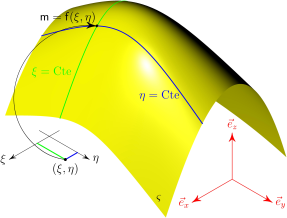
\includegraphics{./asy/fig20230218105342.pdf}

}

\caption{\label{fig-20230218105342}La surface paramétrée \(ς\)}

\end{figure}

\begin{tcolorbox}[enhanced jigsaw, toptitle=1mm, title=\textcolor{quarto-callout-warning-color}{\faExclamationTriangle}\hspace{0.5em}{Exemples à traiter en classe}, colbacktitle=quarto-callout-warning-color!10!white, toprule=.15mm, left=2mm, bottomrule=.15mm, arc=.35mm, breakable, opacityback=0, colframe=quarto-callout-warning-color-frame, bottomtitle=1mm, titlerule=0mm, leftrule=.75mm, opacitybacktitle=0.6, coltitle=black, rightrule=.15mm, colback=white]

Cylindre, cône, sphère. Bien préciser les paramètres et leur domaine de
définition.

\end{tcolorbox}

\hypertarget{courbes-tracuxe9es-sur-une-surface}{%
\subsection{Courbes tracées sur une
surface}\label{courbes-tracuxe9es-sur-une-surface}}

Une courbe de l'espace est généralement définie par un paramétrage
\(t ∈ ]a, b[ \mapsto \point{g}(t)\) (voir
Annexe~\ref{sec-20230213121713}). L'intervalle \(]a, b[\) étant ici
fixé, on se donne deux applications
\(X, Y \colon ]a, b[ \longrightarrow ℝ\), telles que \[
[X(t), Y(t)] ∈ \mathcal{D} \quad \text{pour tout }t ∈ ]a, b[.
\]

Le paramétrage \(t \mapsto \point{g}(t)\) suivant définit alors une
courbe \(\gamma = \point{g}(]a, b[)\) de l'espace (voir
Figure~\ref{fig-20230218141233}) \[
\point{g}(t) = \point{f}[X(t), Y(t)].
\]

Pour tout \(t ∈ ]a, b[\), le point \(\point{g}(t)\) est par construction
contenu dans la surface \(ς\). On dit que \textbf{la courbe \(γ\) est
tracée sur la surface \(ς\)}.

\begin{figure}

{\centering 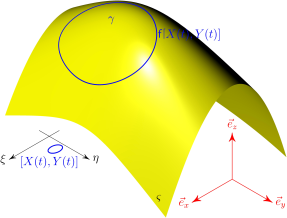
\includegraphics{./asy/fig20230218141233.pdf}

}

\caption{\label{fig-20230218141233}Courbe tracée sur la surface \(ς\)}

\end{figure}

\hypertarget{plan-tangent}{%
\subsection{Plan tangent}\label{plan-tangent}}

La notion de plan tangent est essentielle en théorie des coques, puisque
la plupart des objets tensoriels que nous considèrerons vivent dans le
plan tangent à la configuration initiale ou actuelle. Le plan tangent
est défini comme le plan engendré par l'ensemble des vecteurs tangents à
la surface en un point donné de celle-ci. On voit qu'il faut donc
d'abord définir la notion de vecteur tangent.

Soient \(\point{m} = \point{f}(ξ, η)\) un point de la surface \(ς\) et
\(\vec{v} ∈ ℝ^3\) un vecteur. On dit que le vecteur \(\vec{v}\) est
\textbf{tangent à la surface \(ς\) au point \(\point{m}\)} s'il existe
une courbe \(γ\) tracée sur \(ς\) et passant par \(\point{m}\), telle
que \(\vec{v}\) soit tangent à la courbe \(γ\) au point \(\point{m}\).
On peut alors montrer que l'ensemble \(\mathcal{T}(\point{m}, ς)\) formé
par les vecteurs tangents en \(\point{m}\) à \(ς\) est le plan engendré
par les vecteurs \(\vec{a}_ξ\) et \(\vec{a}_η\) suivants (voir
Figure~\ref{fig-20230219133503}) \[
\vec{a}_ξ(ξ, η) = ∂_ξ \point{f}(ξ, η)
\quad \text{et} \quad
\vec{a}_η(ξ, η) = ∂_η \point{f}(ξ, η).
\]

\begin{figure}

{\centering 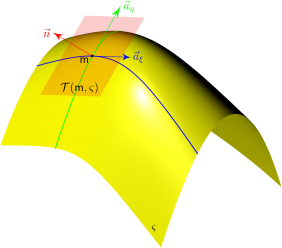
\includegraphics{./asy/fig20230219133503.pdf}

}

\caption{\label{fig-20230219133503}Le plan tangent en \(\point{m}\) est
engendré par les vecteurs \(\vec{a}_ξ\) et \(\vec{a}_η\). Il contient
tous les vecteurs tangents en \(\point{m}\) à des courbes tracées sur la
surface \(ς\).}

\end{figure}

\begin{tcolorbox}[enhanced jigsaw, toptitle=1mm, title=\textcolor{quarto-callout-tip-color}{\faLightbulb}\hspace{0.5em}{Démonstration}, colbacktitle=quarto-callout-tip-color!10!white, toprule=.15mm, left=2mm, bottomrule=.15mm, arc=.35mm, breakable, opacityback=0, colframe=quarto-callout-tip-color-frame, bottomtitle=1mm, titlerule=0mm, leftrule=.75mm, opacitybacktitle=0.6, coltitle=black, rightrule=.15mm, colback=white]

Soit \(\vec{v} ∈ \mathcal{T}(\point{m}, ς)\) l'un de ces vecteurs. Alors
par définition, il existe \(a < b\) et
\(X, Y \colon [a, b] \longrightarrow ℝ\) tels que le vecteur \(\vec{v}\)
soit tangent au point \(\point{m}\) à la courbe \(\Gamma\), définie par
le paramétrage \(t \mapsto \point{g}(t) = \point{f}[X(t), Y(t)]\).
Quitte à changer de paramètre \(t\), on peut toujours supposer que
\(a = -ϵ < 0\), \(b = ϵ > 0\) et que \(γ\) passe par \(\point{m}\) en
\(t = 0\) \[
X(0) = ξ, \quad Y(0) = η \quad \text{et} \quad \point{g}(0) = \point{f}(ξ, η) = \point{m}.
\]

La direction tangente à \(γ\) en \(\point{m}\) est alors donnée par
\(\dot{\point{g}}(0)\), soit en utilisant la règle de dérivation des
fonctions composées \[
\begin{aligned}
\dot{\point{g}}(0)
&= \dot{X}(0) \, ∂_ξ\point{f}[X(0), Y(0)] + \dot{Y}(0) \, ∂_η\point{f}[X(0), Y(0)]\\
&= \dot{X}(0) \, ∂_ξ\point{f}(ξ, η) + \dot{Y}(0) \, ∂_η\point{f}(ξ, η).
\end{aligned}
\]

Puisque \(\vec{v}\) est tangent à \(γ\) en \(\point{m}\), il est
proportionnel au vecteur précédent et on a montré que \textbf{tout
vecteur tangent en \(\point{m}\) à \(ς\) est une combinaison linéaire
des vecteurs \(\vec{a}_ξ\) et \(\vec{a}_η\)}~:
\(\mathcal{T}(\point{m}, ς) ⊂ \Span(\vec{a}_ξ, \vec{a}_η)\).

Inversement, soit \(\vec{v} = λ \, \vec{a}_ξ + μ \, \vec{a}_η\) une
combinaison linéaire de ces deux vecteurs. On définit alors
\([X(t), Y(t)] = (ξ + t \, λ, η + t \, λ)\). Le domaine \(\mathcal{D}\)
étant ouvert, on peut trouver \(ϵ > 0\) tel que
\([X(t), Y(t)] ∈ \mathcal{D}\) pour tout \(t ∈ ]-ϵ, ϵ[\). En d'autres
termes, \(X\) et \(Y\) définissent une courbe tracée sur \(γ\), passant
par \(\point{m} = \point{f}(ξ, η)\) en \(t = 0\). De plus, la direction
tangente à \(γ\) en \(\point{m}\) est \[
\dot{g}(0) = λ \, \vec{a}_ξ + μ \, \vec{a}_η = \vec{v}.
\]

On a donc tracé sur \(ς\) une courbe \(γ\) telle que \(\vec{v}\) soit
tangent à \(γ\) en \(\point{m}\)~: \(\vec{v}\) est bien \textbf{tangent}
à \(ς\) et \textbf{toute combinaison linéaire de \(\vec{a}_ξ\) et
\(\vec{a}_η\) est un vecteur tangent en \(\point{m}\) à \(ς\)}~:
\(\Span(\vec{a}_ξ, \vec{a}_η) ⊂ \mathcal{T}(\point{m}, ς)\). CQFD.

\end{tcolorbox}

Le point \(\point{m}\) est un \textbf{point régulier} de \(ς\) si ces
deux vecteurs sont linéairement indépendants
(\(\vec{a}_ξ \wedge \vec{a}_η = \vec{0}\)). Dans ce cas,
\(\mathcal{T}(\point{m}, ς)\) est le \textbf{plan tangent} à \(ς\) en
\(\point{m}\) et les vecteurs \(\vec{a}_ξ\) et \(\vec{a}_η\) forment la
\textbf{base locale naturelle} associée au paramétrage
\((ξ, η) \mapsto \point{f}(ξ, η)\).

Si ces deux vecteurs sont colinéaires
(\(\vec{a}_ξ \wedge \vec{a}_η = \vec{0}\)), le point \(\point{m}\) est
un \textbf{point singulier}. Le plan tangent n'existe pas en un tel
point.

\begin{tcolorbox}[enhanced jigsaw, toptitle=1mm, title=\textcolor{quarto-callout-note-color}{\faInfo}\hspace{0.5em}{Note}, colbacktitle=quarto-callout-note-color!10!white, toprule=.15mm, left=2mm, bottomrule=.15mm, arc=.35mm, breakable, opacityback=0, colframe=quarto-callout-note-color-frame, bottomtitle=1mm, titlerule=0mm, leftrule=.75mm, opacitybacktitle=0.6, coltitle=black, rightrule=.15mm, colback=white]

On peut montrer que le plan tangent ainsi mis en évidence ne dépend pas
du choix du paramétrage~: il est \textbf{intrinsèque}. L'écriture
\(\mathcal{T}(\point{m}, ς)\) {[}plutôt que \(\mathcal{T}(ξ, η, ς)\){]}
est donc légitime.

\end{tcolorbox}

\hypertarget{vecteur-normal}{%
\subsection{Vecteur normal}\label{vecteur-normal}}

En un point \(\point{m} = \point{f}(ξ, η)\) régulier de la surface
\(ς\), le vecteur \(\vec{a}_ξ \wedge \vec{a}_η\) est perpendiculaire au
plan tangent \(\mathcal{T}(\point{m}, ς)\) (voir
Figure~\ref{fig-20230219133503}). On définit la \textbf{normale unitaire
à \(ς\)} de la façon suivante
\begin{equation}\protect\hypertarget{eq-20230214053253}{}{
\vec{n}(ξ, η) = \frac{\vec{a}_ξ(ξ, η) \wedge \vec{a}_η(ξ, η)}{\lVert \vec{a}_ξ(ξ, η) \wedge \vec{a}_η(ξ, η) \rVert},
}\label{eq-20230214053253}\end{equation} où le dénominateur n'est pas
nul puisque le point \(\point{m}\) est régulier.

\begin{tcolorbox}[enhanced jigsaw, toptitle=1mm, title=\textcolor{quarto-callout-note-color}{\faInfo}\hspace{0.5em}{Note}, colbacktitle=quarto-callout-note-color!10!white, toprule=.15mm, left=2mm, bottomrule=.15mm, arc=.35mm, breakable, opacityback=0, colframe=quarto-callout-note-color-frame, bottomtitle=1mm, titlerule=0mm, leftrule=.75mm, opacitybacktitle=0.6, coltitle=black, rightrule=.15mm, colback=white]

La normale \(\vec{n}\) oriente localement la surface puisqu'elle oriente
son plan tangent \(\mathcal{T}(\point{m}, ς)\) (au sens du
§~\ref{sec-20230213144828}). Cette orientation est néanmoins
\textbf{arbitraire}. En effet, permuter l'ordre de \(ξ\) et \(η\) aurait
conduit à une inversion du sens de \(\vec{n}\) et donc de l'orientation
du plan tangent.

\end{tcolorbox}

\begin{tcolorbox}[enhanced jigsaw, toptitle=1mm, title=\textcolor{quarto-callout-note-color}{\faInfo}\hspace{0.5em}{Note}, colbacktitle=quarto-callout-note-color!10!white, toprule=.15mm, left=2mm, bottomrule=.15mm, arc=.35mm, breakable, opacityback=0, colframe=quarto-callout-note-color-frame, bottomtitle=1mm, titlerule=0mm, leftrule=.75mm, opacitybacktitle=0.6, coltitle=black, rightrule=.15mm, colback=white]

Puisque le plan tangent est une caractéristique intrinsèque de la
surface, la direction normale l'est également. Bien que le vecteur
normal \(\vec{n}\) apparaisse dans l'éq.~(\ref{eq-20230214053253}) comme
une fonction de \(ξ\) et \(η\), on préfèrera dans ce qui suit la
notation \(\vec{n}(\point{m})\).

\end{tcolorbox}

\hypertarget{extension-aux-surfaces-des-notions-introduites-au-sec-20230214053442}{%
\subsection{\texorpdfstring{Extension aux surfaces des notions
introduites au
§~\ref{sec-20230214053442}}{Extension aux surfaces des notions introduites au §~}}\label{extension-aux-surfaces-des-notions-introduites-au-sec-20230214053442}}

À chaque point \(\point{m}\) de la surface est associé un unique plan
tangent, \(\mathcal{T}(\point{m}, ς)\). Dans ce plan, on peut définir,
comme au §~\ref{sec-20230214053442}, l'identité du plan tangent
\(\tens{a}\) et le tenseur antisymétrique fondamental \(\tens{e}\). Ces
deux tenseurs sont des champs (ils dépendent du point d'observation
\(\point{m}\) sur la surface \(ς\)) \textbf{intrinsèques} (ils ne
dépendent pas du choix de la représentation paramétrique de cette
surface)

\[
\tens{a}(\point{m}) = \tens{I} - \vec{n}(\point{m}) ⊗ \vec{n}(\point{m})
\quad \text{et} \quad
\tens{e}(\point{m}) ⋅ \vec{v} = \vec{v} \wedge \vec{n}(\point{m}) \quad \text{pour tout } \vec{v} ∈ ℝ^3.
\]

Ces champs de tenseurs ont bien sûr les mêmes propriétés que leurs
homologues introduits sur un plan fixe.

\hypertarget{repruxe9sentation-cartuxe9sienne-locale-dune-surface}{%
\subsection{Représentation cartésienne locale d'une
surface}\label{repruxe9sentation-cartuxe9sienne-locale-dune-surface}}

Soit \(\point{m} ∈ ς\) un point régulier de la surface \(ς\) et
\((\vec{e}_x, \vec{e}_y)\) une base orthonormée de son plan tangent
\(\mathcal{T}(\point{m}, ς)\). En posant
\(\vec{e}_z = \vec{n}(\point{m})\), on construit ainsi un repère
cartésien orthonormé de l'espace
\((\point{m}, \vec{e}_x, \vec{e}_y, \vec{e}_z)\). Dans ce repère, il
existe une fonction \(g(x, y)\), définie et dérivable au voisinage de
l'origine \(\point{m} (\)x = 0\$, \(y = 0\)), telle que l'équation
cartésienne de la surface \(ς\) s'écrive, au voisinage de \(\point{m}\)
\[
z = g(x, y) \quad \text{avec} \quad g(0, 0) = 0 \quad \text{et} \quad ∂_xg(0, 0) = ∂_yg(0, 0) = 0.
\]

\begin{tcolorbox}[enhanced jigsaw, toptitle=1mm, title=\textcolor{quarto-callout-tip-color}{\faLightbulb}\hspace{0.5em}{Démonstration}, colbacktitle=quarto-callout-tip-color!10!white, toprule=.15mm, left=2mm, bottomrule=.15mm, arc=.35mm, breakable, opacityback=0, colframe=quarto-callout-tip-color-frame, bottomtitle=1mm, titlerule=0mm, leftrule=.75mm, opacitybacktitle=0.6, coltitle=black, rightrule=.15mm, colback=white]

Soit \((ξ, η) \mapsto \point{f}(ξ, η)\) un paramétrage de la surface
\(ς\). On peut toujours supposer que \(\point{m} = \point{f}(0, 0)\).
Soient \(φ_x\) et \(φ_y\) les fonctions définies de la façon suivante \[
φ_x(ξ, η) = \vec{e}_x ⋅ \tens{a}(\point{m}) ⋅ \altvec{\point{mm}'} \quad \text{et} \quad φ_y(ξ, η) = \vec{e}_y ⋅ \tens{a}(\point{m}) ⋅ \altvec{\point{mm}'}
\] où \(\point{m'} = \point{f}(ξ, η)\) désigne un point voisin de
\(\point{m}\) sur la surface \(ς\) et \(\tens{a}\) est l'identité du
plan tangent en \(\point{m}\). La base
\((\vec{e}_x, \vec{e}_y, \vec{e}_z)\) étant orthonormée, on remarque que
\[
\tens{a} = \tens{I} - \vec{n} ⊗ \vec{n} = \vec{e}_x ⊗ \vec{e}_x + \vec{e}_y ⊗ \vec{e}_y + \vec{e}_z ⊗ \vec{e}_z - \vec{n} ⊗ \vec{n} = \vec{e}_x ⊗ \vec{e}_x + \vec{e}_y ⊗ \vec{e}_y,
\] puisque \(\vec{e}_z = \vec{n}\) par construction. On définit alors la
fonction \(φ\) \[
φ(ξ, η) = \bigl[φ_x(ξ, η), φ_y(ξ, η)\bigr],
\] qui extrait les coordonnées dans le repère
\((\point m, \vec e_x, \vec e_y)\) de la projection orthogonale du point
courant \(\point{m}'=\point{f}(ξ, η)\) sur le plan tangent
\(\mathcal{T}(\point{m}, ς)\). Le jacobien de \(φ\) vaut \[
\begin{vmatrix}
\vec{e}_x ⋅ \tens{a} ⋅ \vec{a}_{ξ}(ξ, η) & \vec{e}_x ⋅ \tens{a} ⋅ \vec{a}_{η}(ξ, η)\\
\vec{e}_y ⋅ \tens{a} ⋅ \vec{a}_{ξ}(ξ, η) & \vec{e}_y ⋅ \tens{a} ⋅ \vec{a}_{η}(ξ, η)
\end{vmatrix}
= \vec{e}_z ⋅ \bigl[ \bigl( \tens{a} ⋅ \vec{a}_ξ(ξ, η) \bigr) \wedge \bigl( \tens{a} ⋅ \vec{a}_η(ξ, η) \bigr) \bigr]
\]

En \((ξ, η) = (0, 0)\), on a
\(\tens{a} ⋅ \vec{a}_ξ(0, 0) = \vec{a}_ξ(0, 0)\) et
\(\tens{a} ⋅ \vec{a}_η(0, 0) = \vec{a}_η(0, 0)\). Le jacobien vaut donc
\(\lVert \vec{a}_ξ(0, 0) \wedge \vec{a}_η(0, 0) \rVert\), qui est
non-nul puisque \(\point{m}\) est un point régulier. La différentielle
de \(φ\) est donc inversible en \((0, 0)\). Le théorème d'inversion
locale garantit alors qu'on peut inverser localement au voisinage de
\((ξ = 0, η = 0)\) la fonction \(φ\). Soit \(ψ\) son inverse~; on a
alors, pour tous \((x, y)\) suffisamment petits~:
\(φ[ψ(x, y)] = (x, y)\). En d'autres termes \[
\tens{a} ⋅ \altvec{\point{mm}'} = x \, \vec{e}_x + y \, \vec{e}_y, \quad \text{avec} \quad \point m' = \point{f}[ψ(x, y)].
\]

On définit alors la fonction \(g(x, y)\) \[
g(x, y) = \vec{e}_z ⋅ \altvec{\point{mm}'}, \quad \text{avec} \quad \point{m}'= \point{f}[ψ(x, y)].
\]

Comme \(\tens{a} + \vec{e}_z ⊗ \vec{e}_z = \tens I\), on obtient \[
\altvec{\point{mm}'} = x \, \vec{e}_x + y \, \vec{e}_y + g(x, y) \, \vec{e}_z,
\] pour tout point \(\point{m}'\) de \(ς\), suffisamment proche de
\(\point{m}\). On a donc bien construit localement une représentation
cartésienne de la surface \(ς\). Bien sûr, lorsque \(x = y = 0\), le
point \(\point{m}'\) coïncide avec \(\point{m}\), donc \(g(0, 0) = 0\).
Par ailleurs, puisque le plan tangent en \(\point{m}\) à \(ς\) est le
plan \((\point{m}, \vec{e}_x, \vec{e}_y)\), on a également
\(∂_x g(0, 0) = ∂_y g(0, 0) = 0\). Pour le voir, il suffit d'observer
que l'on peut considérer les coordonnées \((x, y)\) comme un paramétrage
de la surface \(ς\). Ainsi, \(\point{g}(x, y)\) est un point de \(ς\)
pour tous \(x, y\) suffisamment petits, en posant \[
\point{g}(x, y)=\point{m} + x \, \vec{e}_x + y \, \vec{e}_y + g(x, y) \, \vec{e}_z.
\]

La base locale naturelle associée est \[
\vec{a}_x(x, y) = \vec{e}_x + ∂_x g(x, y) \, \vec{e}_z \quad \text{et} \quad \vec{a}_y(x, y) = \vec{e}_y + ∂_y g(x, y) \, \vec{e}_z.
\]

Les vecteurs \(\vec{a}_x(0, 0)\) et \(\vec{a}_y(0, 0)\) sont tangents à
\(ς\) en \(\point{m}\)~: ils sont donc contenus dans le plan tangent en
\(\point{m}\), et leur composante selon \(\vec{e}_z\) est nulle.

\end{tcolorbox}

\hypertarget{courbure-des-surfaces-1}{%
\section{Courbure des surfaces}\label{courbure-des-surfaces-1}}

\hypertarget{tenseur-de-courbure}{%
\subsection{Tenseur de courbure}\label{tenseur-de-courbure}}

Soient \(\point{m}\) un point régulier d'une surface \(ς\) et
\(\vec{t}\) un vecteur unitaire, tangent à \(ς\) en \(\point{m}\). Le
point \(\point{m}\) et les vecteurs \(\vec{t}\) et
\(\vec{n}(\point{m})\) définissent un plan \(π\) qui rencontre la
surface \(ς\) le long de la courbe \(γ\) (voir
Figure~\ref{fig-20230219200134}). Cette courbe est une courbe plane,
puisqu'elle est par construction contenue dans le plan \(π\). Sa
courbure en \(\point{m}\) est donc une notion connue (voir
§~\ref{sec-20230214055209}).

\begin{figure}

{\centering 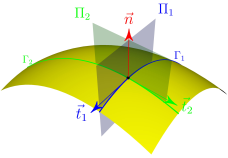
\includegraphics{./asy/fig20230219200134.pdf}

}

\caption{\label{fig-20230219200134}Le plan \(π\), passant par
\(\point{m} ∈ ς\) et contenant la normale \(\vec n(\point{m})\) ainsi
que le vecteur \(\vec{t} ∈ \mathcal{T}(\point{m}, ς)\) donné, rencontre
la surface \(ς\) le long de la courbe \(γ\). La courbure de \(γ\) en
\(\point{m}\) est \(\vec{t} ⋅ \tens{b} ⋅ \vec{t}\).}

\end{figure}

Si la surface \(ς\) est suffisamment régulière en \(\point{m}\), alors
on il existe un tenseur \(\tens{b}(\point{m})\) tel que la courbure de
\(γ\) au point \(\point{m}\) soit donnée par l'expression~:
\(\vec{t} ⋅ \tens{b}(\point{m}) ⋅ \vec{t}\). Le tenseur
\(\tens{b}(\point{m})\) ainsi introduit est le \textbf{tenseur de
courbure de la surface \(ς\) au point \(\point{m}\)}. C'est un tenseur
du plan tangent en \(\point{m}\), symétrique.

\begin{tcolorbox}[enhanced jigsaw, toptitle=1mm, title=\textcolor{quarto-callout-tip-color}{\faLightbulb}\hspace{0.5em}{Démonstration}, colbacktitle=quarto-callout-tip-color!10!white, toprule=.15mm, left=2mm, bottomrule=.15mm, arc=.35mm, breakable, opacityback=0, colframe=quarto-callout-tip-color-frame, bottomtitle=1mm, titlerule=0mm, leftrule=.75mm, opacitybacktitle=0.6, coltitle=black, rightrule=.15mm, colback=white]

Pour établir l'existence du tenseur \(\tens{b}\) au point
\(\point{m} ∈ ς\), on considère une représentation cartésienne locale
\((x, y) \mapsto g(x, y)\) de la surface au voisinage de \(\point{m}\).
Ainsi tout point \(\point{m}'\) suffisamment proche de \(\point{m}\) sur
\(ς\) s'écrit \[
\point{m}' = \point{m} + x \, \vec{e}_x + y \, \vec{e}_y + g(x, y) \, \vec{e}_z ∈ ς,
\] où \((\vec{e}_x, \vec{e}_y)\) désigne une base orthonormée du plan
tangent \(\mathcal{T}(\point{m}, ς)\) et \(\vec{e}_z = \vec{n}\). Tout
point \(\point{m}'\) du plan \(π\) peut par ailleurs s'écrire \[
\point{m}' = \point{m} + r \, \vec{t} + z \, \vec{e}_z = \point{m} + r \, t_x \, \vec{e}_x + r \, t_y \, \vec{e}_y + z \, \vec{e}_z ∈ π.
\] Un point \(\point{m}'\) de la courbe \(γ\) doit safisfaire
simultanément les représentations précédentes. On en déduit la
représentation paramétrique de \(γ\) au voisinage de \(\point{M}\) \[
x = r \, t_x, \quad y = r \, t_y \quad \text{et} z = g(r \, t_x, r \, t_y),
\] où le (petit) paramètre est \(r\). Les dérivées premières de \(g\)
étant nulles, on obtient à l'ordre le plus bas en r
\begin{equation}\protect\hypertarget{eq-20230214084729}{}{
z = g(r \, t_x, r \, t_y) = \frac{r^2}{2} \, \bigl[ t_x^2 \, ∂_{xx}^2 g(0, 0) +2t_x \, t_y \, ∂_{xy}^2g(0, 0) + t_y^2 \, ∂_{yy}^2g(0, 0) \bigr] + o\bigl( r^2 \bigr).
}\label{eq-20230214084729}\end{equation}

Soit \(\tens{b}\) la \textbf{hessienne} de \(g\) à l'origine \[
\tens{b} = ∂_{αβ}^2 g(0, 0) \, \vec{e}_α ⊗ \vec{e}_β.
\]

Le tenseur \(\tens{b}\) ainsi défini est un tenseur du plan tangent
\(\mathcal{T}(\point{m}, ς)\), symétrique. De plus, l'équation
(\ref{eq-20230214084729}) se met sous la forme \[
z = \frac{r^2}{2} \, \vec{t} ⋅ \tens{b} ⋅ \vec{t} + o\bigl( r^2 \bigr).
\]

On reconnaît, dans la base cartésienne \((\vec{t}, \vec{e}_z)\) du plan
\(π\), l'équation d'une parabole et le terme en \(r^2 / 2\) correspond à
la courbure au sommet de cette parabole (soit, au point \(\point{m}\)).
On a donc bien mis la courbure de \(γ\) en \(\point{m}\) sous la forme
\(\vec{t} ⋅ \tens{b} ⋅ \vec{t}\), où \(\tens{b}\) est la hessienne de
\(g\) à l'origine.

Le tenseur de courbure \(\tens{b}\) a été construit ici dans un système
de coordonnées curviligne très particulier. Pour conclure cette
démonstration, il faut montrer que ce tenseur est bien
\textbf{intrinsèque}, c'est-à-dire indépendant de la représentation
paramétrique de \(ς\). C'est en fait immédiat, puisque \(\tens{b}\)
relie le vecteur unitaire du plan tangent \(\vec{t}\) à la courbure
\(\vec{t} ⋅ \tens{b} ⋅ \vec{t}\) d'une courbe plane, ces objets étant
eux-mêmes définis de façon intrinsèque. On écrira donc
\(\tens{b}(\point{m})\) et pas \(\tens{b}(ξ, η)\) pour désigner le
tenseur de courbure au point \(\point{m}\) de \(ς\).

\end{tcolorbox}

\hypertarget{courbures-principales-et-classification-des-points-ruxe9guliers}{%
\subsection{Courbures principales et classification des points
réguliers}\label{courbures-principales-et-classification-des-points-ruxe9guliers}}

Le tenseur de courbure \(\tens{b}\) étant symétrique, il est
diagonalisable dans une base orthonormée du plan tangent
\(\mathcal{T}(\point{m}, ς)\) et on peut introduire les
\textbf{courbures principales} \(b_{\mathrm{I}}\) et
\(b_{\mathrm{II}}\), qui sont les valeurs propres de ce tenseur. On
conviendra d'ordonner ces valeurs propres de façon à ce que
\(b_{\mathrm{I}} \leq b_{\mathrm{II}}\). Les courbures principales sont
les valeurs extrêmes de la courbure en \(\point{m}\) de la courbe plane
\(γ\) introduite ci-dessus.

\begin{tcolorbox}[enhanced jigsaw, toptitle=1mm, title=\textcolor{quarto-callout-tip-color}{\faLightbulb}\hspace{0.5em}{Démonstration}, colbacktitle=quarto-callout-tip-color!10!white, toprule=.15mm, left=2mm, bottomrule=.15mm, arc=.35mm, breakable, opacityback=0, colframe=quarto-callout-tip-color-frame, bottomtitle=1mm, titlerule=0mm, leftrule=.75mm, opacitybacktitle=0.6, coltitle=black, rightrule=.15mm, colback=white]

Pour montrer ce résultat, on introduit les directions principales de
courbure \(\vec{t}_{\mathrm{I}}\) et \(\vec{t}_{\mathrm{II}}\) (vecteurs
unitaires orthogonaux), de sorte que \[
\tens{b} = b_{\mathrm{I}} \, \vec{t}_{\mathrm{I}} ⊗ \vec{t}_{\mathrm{I}} + b_{\mathrm{II}} \, \vec{t}_{\mathrm{II}} ⊗ \vec{t}_{\mathrm{II}}.
\]

Les vecteurs \(\vec{t}_{\mathrm{I}}\) et \(\vec{t}_{\mathrm{II}}\)
forment une base orthonormée, dans laquelle on peut décomposer le
vecteur \(\vec{t}\)~:
\(\vec{t} = \cos θ \, \vec{t}_{\mathrm{I}} + \sin θ \, \vec{t}_{\mathrm{II}}\).
La courbure de \(γ\) en \(\point{m}\) a donc pour expression \[
\vec{t} ⋅ \tens{b} ⋅ \vec{t} = \cos^2 θ \, b_{\mathrm{I}} + \sin^2 θ \, b_{\mathrm{II}},
\] dont les valeurs extrêmes sont bien obtenues pour \(θ=0\)
(\(\vec{t} = \vec{t}_{\mathrm{I}}\)) ou \(θ = π/2\)
(\(\vec{t} = \vec{t}_{\mathrm{II}}\)).

\end{tcolorbox}

Comme pour une courbe plane, le signe des courbures principales
\textbf{dépend de l'orientation de \(ς\)} (de la normale \(\vec{n}\)).
Les produits \(b_{\mathrm{I}} \, \vec{n}\) et
\(b_{\mathrm{II}} \, \vec{n}\) sont quant à eux intrinsèques et
indiquent de quel côté la surface oriente sa courbure. En effet les deux
centres de courbure associés aux courbures principales sont situé en
\(\point{m} + \vec{n} / b_{\mathrm{I}}\) et
\(\point{m} + \vec{n} / b_{\mathrm{II}}\).

\begin{tcolorbox}[enhanced jigsaw, toptitle=1mm, title=\textcolor{quarto-callout-warning-color}{\faExclamationTriangle}\hspace{0.5em}{Exemples à traiter en classe}, colbacktitle=quarto-callout-warning-color!10!white, toprule=.15mm, left=2mm, bottomrule=.15mm, arc=.35mm, breakable, opacityback=0, colframe=quarto-callout-warning-color-frame, bottomtitle=1mm, titlerule=0mm, leftrule=.75mm, opacitybacktitle=0.6, coltitle=black, rightrule=.15mm, colback=white]

Sphère, cylindre.

\end{tcolorbox}

On peut introduire une classification des points réguliers \(\point{m}\)
d'une surface en fonction des signes des courbures principales
\(b_{\mathrm{I}}\) et \(b_{\mathrm{II}}\).

\begin{itemize}
\tightlist
\item
  Si \(b_{\mathrm{I}} \, b_{\mathrm{II}} > 0\) (courbures principales
  non-nulles et de même signe), le point \(\point{m}\) est dit
  \textbf{elliptique}.
\item
  Si \(b_{\mathrm{I}} \, b_{\mathrm{II}} < 0\) (courbures principales
  non-nulles et de signes contraires), le point \(\point{m}\) est dit
  \textbf{hyperbolique}.
\item
  Si l'une seulement des deux courbures principales est nulle, le point
  \(\point{m}\) est \textbf{parabolique}.
\item
  Si les deux courbures principales sont nulles, le point \(\point{m}\)
  est un \textbf{méplat}.
\item
  Si les deux courbures principales sont égales et non-nulles, le
  tenseur de courbure est diagonal et la courbure de la courbe \(γ\) est
  indépendante du vecteur \(\vec{t}\)~; le point \(\point{m}\) est un
  point \textbf{ombilic}.
\end{itemize}

\hypertarget{courbure-moyenne-courbure-gaussienne}{%
\subsection{Courbure moyenne, courbure
gaussienne}\label{courbure-moyenne-courbure-gaussienne}}

Les courbures \textbf{moyenne \(h\)} et \textbf{gaussienne \(k\)} de la
surface sont définies à partir des courbures principales
\(b_{\mathrm{I}}\) et \(b_{\mathrm{II}}\) \[
h = \tfrac{1}{2} \, \bigl( b_{\mathrm{I}} + b_{\mathrm{II}} \bigr) \quad \text{et} \quad k = b_{\mathrm{I}} \, {b_\mathrm{II}}.
\]

Le tenseur de courbure \(\tens b\) est un tenseur du plan tangent
\(\mathcal{T}(\point{m}, ς)\)~: il peut donc être considéré comme le
représentant d'un \textbf{endomorphisme} de
\(\mathcal{T}(\point{m}, ς)\) (espace vectoriel de dimension 2). Les
courbures moyenne et gaussienne apparaissent alors comme les
\textbf{invariants} de \(\tens{b}\) \[
h = \tfrac{1}{2} \tr \tens{b} \quad \text{et} \quad k = \det_{2 × 2} \tens{b} = \det_{3 × 3} \bigl( \tens{b} + \vec{n} ⊗ \vec{n} \bigr)
\] (les notations \(\det_{2 × 2}\) et \(\det_{3 × 3}\) sont précisées
dans l'annexe §~\ref{sec-20230213110532}). Le point \(\point{m}\) de la
surface \(ς\) est elliptique, parabolique ou hyperbolique si la courbure
gaussienne est positive, nulle ou négative, respectivement. Par
ailleurs, le théorème de Cayley--Hamilton permet d'écrire que
\(\tens{b}\) annule son polyôme caractéristique \[
\tens{b} ⋅ \tens{b} - 2h \, \tens{b} + k \, \tens{a} = \tens{0}.
\]

\bookmarksetup{startatroot}

\hypertarget{sec-20230314085944}{%
\chapter{Transformations d'une coque}\label{sec-20230314085944}}

Une coque est une structure dont l'une des dimensions
(\textbf{l'épaisseur}) est grande devant les deux autres. Il est alors
naturel de chercher à décrire l'état de la coque par un ensemble de
champs construits sur son \textbf{feuillet de référence} seulement. On
construit ainsi une théorie surfacique de coque. La plus simple de ces
théories est la théorie de Kirchhoff--Love, dans laquelle on suppose que
l'état mécanique de la coque est complètement défini par les changements
de géométrie de son feuillet de référence. Dans ce chapitre, on définit
donc des grandeurs tensorielles permettant de mesurer ces changements de
géométrie. On veillera à ce que les \textbf{déformations généralisées}
ainsi définies permettent bien d'identifier les mouvements de corps
solides.

\hypertarget{points-matuxe9riels-2d}{%
\section{Points matériels 2D}\label{points-matuxe9riels-2d}}

Vue comme un solide tridimensionnel, la coque est constituée de
\textbf{points matériels 3D}, qui correspondent aux points matériels
classiques de la mécanique des milieux continus. Si le matériau
constitutif de la coque est standard (de Cauchy), \textbf{chaque point
matériel 3D possède 3 degrés de liberté de translation}.

Vue comme un solide surfacique, la coque est constituée de
\textbf{points matériels 2D}. Un point matériel 2D correspond
mathématiquement à un point géométrique du feuillet de référence et
physiquement à \textbf{l'ensemble des points matériels 3D} de la coque
(vue comme un solide tridimensionnel) \textbf{situés sur la même normale
au feuillet de référence} (voir Figure~\ref{fig-20230302052722}).

La translation d'ensemble des points matériels 3D permet de définir une
translation du point matériel 2D, soit \textbf{3 degrés de liberté de
translation}.

La translation \textbf{relative} des points matériels 3D permet
également de définir \textbf{2 degrés de liberté de rotation}
supplémentaires. Les points matériels 2D ne possèdent pas de degré de
liberté en rotation selon la normale au feuillet de référence.

\begin{figure}

{\centering 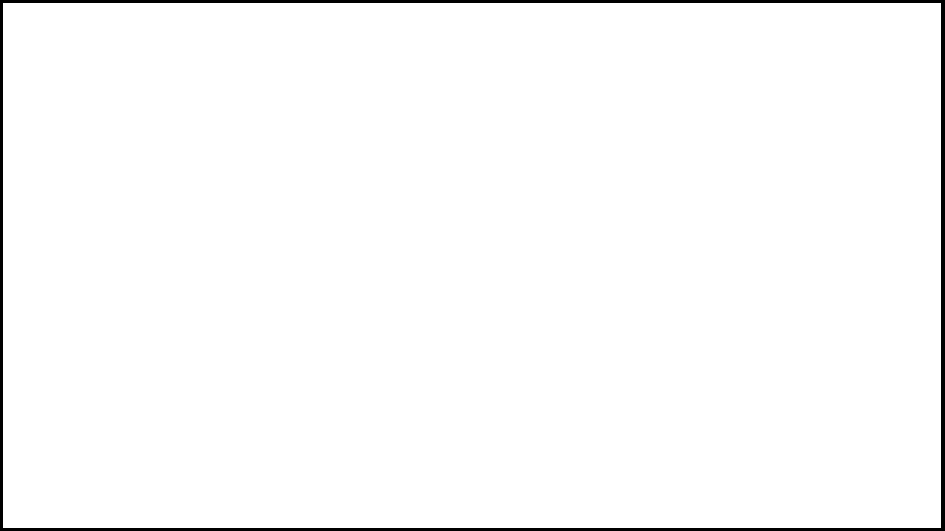
\includegraphics{./croquis/blanc.pdf}

}

\caption{\label{fig-20230302052722}Un point matériel 2D correspond à un
ensemble de points matériels 3D, tous situés initialement sur la même
fibre. Le mouvement d'ensemble des points matériels 3D définit la
translation du point matériel 2D~; leur mouvement relatif définit deux
rotations du point matériel 2D.}

\end{figure}

\hypertarget{coordonnuxe9es-matuxe9rielles-des-points-de-la-coque}{%
\section{Coordonnées matérielles des points de la
coque}\label{coordonnuxe9es-matuxe9rielles-des-points-de-la-coque}}

On notera \(\Sigma\) et \(\varsigma\) les feuillets de référence de la
coque dans les configurations initiale et actuelle, respectivement. Ces
surfaces sont définies par les paramétrages \[
(\Xi, \Eta) \mapsto \point{M} = \point{F}(\Xi, \Eta) \in \Sigma
\quad \text{et} \quad
(\xi, \eta) \mapsto \point{m} = \point{f}(\xi, \eta) \in \varsigma.
\] (noter l'utilisation des majuscules sur la configuration initiale et
des minuscules sur la configuration actuelle). Le mouvement de la coque
peut alors être défini par la transformation des coordonnées curvilignes
\[
(\Xi, \Eta) \mapsto (\xi, \eta) = \Phi(\Xi, \Eta).
\]

On peut ainsi, pour tout point matériel de la coque, associer à sa
position \(\point{M} \in \Sigma\) sur la configuration initiale, sa
position \(\point{m} \in \varsigma\) sur la configuration actuelle de la
façon suivante \[
\point{M} = \point{F}(\Xi, \Eta) \quad \mapsto \quad \point{m} = \point{f} [ \Phi(\Xi, \Eta) ].
\]

La représentation précédente de la transformation de la coque est d'une
grande généralité, mais conduit à certaines lourdeurs mathématiques. On
conviendra dans ce cours que les fonctions \(\point{F}\) et
\(\point{f}\) sont choisies de sorte \(\xi = \Xi\) et \(\eta = \Eta\).
Ainsi, \((\xi, \eta)\) sont les coordonnées curvilignes du \textbf{même
point matériel}, dans les deux configurations. On parle de
\textbf{coordonnées matérielles}~; elles permettent d'identifier un
point matériel. Ainsi, le point matériel de coordonnées matérielles
\((\xi, \eta)\) occupe la position
\(\point{M} = \point{F}(\xi, \eta) \in \Sigma\) dans la configuration
initiale. Il est transporté en
\(\point{m} = \point{f}(\xi, \eta) \in \varsigma\) dans la configuration
actuelle (voir Figure~\ref{fig-20230302053622}).

\begin{figure}

{\centering 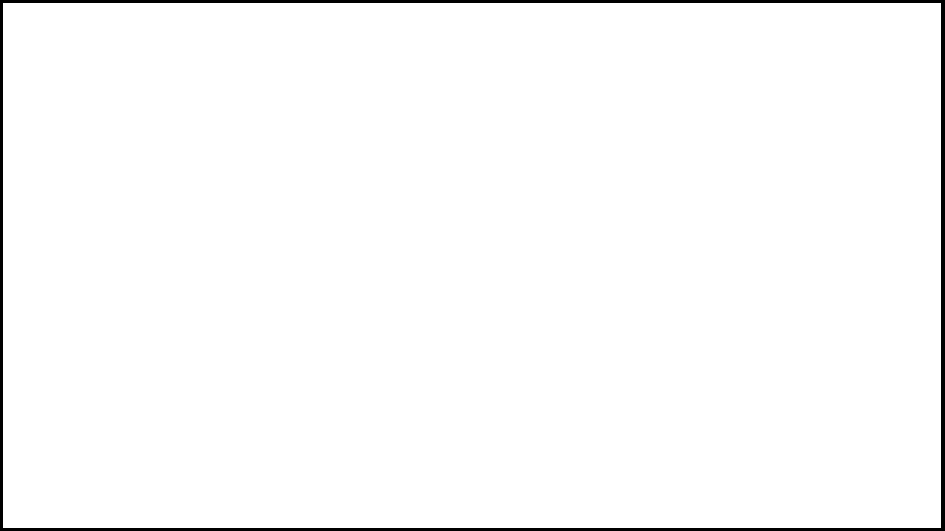
\includegraphics{./croquis/blanc.pdf}

}

\caption{\label{fig-20230302053622}On utilise les mêmes coordonnées
curvilignes \(\xi\) et \(\eta\) pour paramétrer les configurations
initiale \(\Sigma\) et actuelle \(\varsigma\). Ces coordonnées
curvilignes sont des coordonnées \textbf{matérielles}.}

\end{figure}

\hypertarget{duxe9placement}{%
\section{Déplacement}\label{duxe9placement}}

Soit un point matériel de la coque occupant les positions \(\point{M}\)
et \(\point{m}\) dans les configurations initiale et actuelle. Le
\textbf{déplacement} de ce point matériel est par définition le vecteur
(voir Figure~\ref{fig-20230302053622}) \[
\vec{u}(\point{M}) = \altvec{\point{Mm}} = \point{m} - \point{M}.
\]

Il correspond à la translation du point matériel entre les deux
configurations. Le champ de déplacement ainsi défini est une quantité
lagrangienne (définie sur la configuration de référence). On peut aussi
considérer le champ des déplacements comme une fonction des coordonnées
matérielles \(\xi\) et \(\eta\) \[
\vec{u}(\xi, \eta) = \point{f}(\xi, \eta) - \point{F}(\xi, \eta).
\]

La configuration actuelle de la coque est ainsi complètement définie par
la configuration initiale et le champ des déplacements, puisque la
relation précédente s'inverse trivialement \[
\point{f}(\xi, \eta) = \point{F}(\xi, \eta) + \vec{u}(\xi, \eta).
\]

En particulier, on peut exprimer les vecteurs
\((\vec{a}_\xi, \vec{a}_\eta)\) de la base locale naturelle actuelle en
fonction des vecteurs \(\vec{A}_\xi\) et \(\vec{A}_\eta\) de la base
locale naturelle initiale \[
\vec{a}_\xi(\xi, \eta) = \partial_\xi \point{f}(\xi, \eta) = \partial_\xi \point{F}(\xi, \eta) + \partial_\xi \vec{u}(\xi, \eta) = \vec{A}_\xi(\xi, \eta) + \partial_\xi \vec{u}(\xi, \eta).
\]

On omettra souvent la dépendance en \(\xi\) et \(\eta\) en écrivant
simplement \begin{equation}\protect\hypertarget{eq-20230314094617}{}{
\vec{a}_\xi = \vec{A}_\xi + \partial_\xi \vec{u} \quad \text{et} \quad \vec{a}_\eta = \vec{A}_\eta + \partial_\eta \vec{u}.
}\label{eq-20230314094617}\end{equation}

\hypertarget{transport-dun-vecteur-matuxe9riel}{%
\section{Transport d'un vecteur
matériel}\label{transport-dun-vecteur-matuxe9riel}}

Soient deux points matériels infiniment proches, de coordonnées
matérielles \((\xi, \eta)\) et
\((\xi_1 = \xi + \D\xi, \eta_1 = \eta + \D\eta)\) (voir
Figure~\ref{fig-20230302054334}). Le \emph{vecteur matériel} constitué
par ces deux points correspond dans la position initiale au vecteur
géométrique suivant \[
\D\altvec{\point{M}} = \altvec{\point{MM}_1} = \point{M}_1 - \point{M},
\] avec \[
\point{M} = \point{F}(\xi, \eta)\] et \[
\begin{aligned}[b]
\point{M}_1 &= \point{F}(\xi_1, \eta_1) = \point{F}(\xi + \D\xi, \eta + \D\eta) = \point{F}(\xi, \eta) + \partial_\xi \point{F}(\xi, \eta) \, \D\xi + \partial_\eta \point{F}(\xi, \eta) \, \D\eta\\
&= \point{M} + \vec{A}_\xi \, \D \xi + \vec{A}_\eta \, \D \eta,
\end{aligned}
\] soit, en regroupant les résultats précédents
\begin{equation}\protect\hypertarget{eq-20230301170119}{}{
\D \altvec{\point{M}} = \vec{A}_\xi \, \D \xi + \vec{A}_\eta \, \D \eta.
}\label{eq-20230301170119}\end{equation}

En d'autres termes, \(\D\xi\) et \(\D\eta\) sont les coordonnées du
vecteur matériel \(\D\altvec{\point{M}}\) dans la base
\((\vec{A}_\xi, \vec{A}_\eta)\). Cette base n'est en général \textbf{pas
orthonormée}. Il n'est donc en général pas vrai que \[
\D \xi = \vec{A}_\xi \cdot \D \altvec{\point{M}}, \quad \text{ni que} \quad \D \eta = \vec{A}_\eta \cdot \D \altvec{\point{M}}.
\]

Pour retrouver des formules de ce type, il est nécessaire d'introduire
la \textbf{base duale} \((\vec{A}_\xi^\ast, \vec{A}_\eta^\ast)\) de la
base locale naturelle, définie par les relations suivantes
\begin{equation}\protect\hypertarget{eq-20230301165727}{}{
\vec{A}_\xi^\ast \cdot \vec{A}_\xi = \vec{A}_\eta^\ast \cdot \vec{A}_\eta = 1
\quad \text{et} \quad
\vec{A}_\xi^\ast \cdot \vec{A}_\eta = \vec{A}_\eta^\ast \cdot \vec{A}_\xi = 0,
}\label{eq-20230301165727}\end{equation} ainsi que \[
\vec{A}_\xi^\ast \cdot \vec{N} = \vec{A}_\eta^\ast \cdot \vec{N} = 0.
\]

\begin{tcolorbox}[enhanced jigsaw, toptitle=1mm, title=\textcolor{quarto-callout-note-color}{\faInfo}\hspace{0.5em}{Note}, colbacktitle=quarto-callout-note-color!10!white, toprule=.15mm, left=2mm, bottomrule=.15mm, arc=.35mm, breakable, opacityback=0, colframe=quarto-callout-note-color-frame, bottomtitle=1mm, titlerule=0mm, leftrule=.75mm, opacitybacktitle=0.6, coltitle=black, rightrule=.15mm, colback=white]

Les relations (\ref{eq-20230301165727}) définissent bien de manière
unique deux vecteurs \(\vec{A}_\xi^\ast\) et \(\vec{A}_\eta^\ast\), dont
on peut montrer qu'ils sont linéairement indépendants si \(\vec{A}_\xi\)
et \(\vec{A}_\eta\) le sont.

Lorsqu'on utilise la convention de sommation d'Einstein, il est courant
de noter ces vecteurs avec un indice supérieur (indice
\textbf{contravariant}) \[
\vec{A}_\xi^\ast = \vec{A}^\xi \quad \text{et} \quad \vec{A}_\eta^\ast = \vec{A}^\eta.
\]

Nous n'utiliserons pas cette convention, ni les notations associées dans
le présent cours.

\end{tcolorbox}

En combinant les relations (\ref{eq-20230301170119}) et
(\ref{eq-20230301165727}), on obtient alors les expressions
\begin{equation}\protect\hypertarget{eq-20230301170457}{}{
\D \xi = \vec{A}_\xi^\ast \cdot \D \altvec{\point{M}} \quad \text{et} \quad \D \eta = \vec{A}_\eta^\ast \cdot \D \altvec{\point{M}},
}\label{eq-20230301170457}\end{equation} qui montrent l'intérêt de la
base duale. L'expression (\ref{eq-20230301170119}) est par ailleurs
vraie également dans la configuration actuelle, où le vecteur matériel
correspond alors au vecteur géométrique \[
\D \altvec{\point{m}} = \vec{a}_\xi \, \D \xi + \vec{a}_\eta \, \D \eta,
\] soit, en introduisant les relations (\ref{eq-20230301170457})
\begin{equation}\protect\hypertarget{eq-20230301171229}{}{
\D \altvec{\point{m}} = \vec{a}_\xi \, \bigl( \vec{A}_\xi^\ast \cdot \D \altvec{\point{M}} \bigr) + \vec{a}_\eta \, \bigl( \vec{A}_\eta^\ast \cdot \D \altvec{\point{M}} \bigr) = \tens{F} \cdot \D \altvec{\point{M}},
}\label{eq-20230301171229}\end{equation} où \textbf{l'application
linéaire tangente \(\tens{F}\)} est définie de la façon suivante
\begin{equation}\protect\hypertarget{eq-20230314094713}{}{
\tens{F} = \vec{a}_\xi \otimes \vec{A}_\xi^\ast + \vec{a}_\eta \otimes \vec{A}_\eta^\ast.
}\label{eq-20230314094713}\end{equation}

L'application linéaire tangente \(\tens{F}\) permet d'exprimer le
transport d'un vecteur matériel entre les configurations initiale et
actuelle à l'aide de la relation (\ref{eq-20230301171229}). Il joue donc
le même rôle que le tenseur du même nom de la mécanique des milieux
continus. On prendra garde néanmoins au fait que \(\tens{F}\) n'est pas
un tenseur inversible de l'espace. En effet \[
\tens{F} \cdot \vec{N} = \vec{n} \cdot \tens{F} = \vec{0},
\] ce qui montre que \(\tens{F}\) représente un endomorphisme du plan
tangent \(\mathcal{T}(\point{M}, \Sigma)\) vers le plan tangent
\(\mathcal{T}(\point{m}, \varsigma)\).

\begin{tcolorbox}[enhanced jigsaw, toptitle=1mm, title=\textcolor{quarto-callout-note-color}{\faInfo}\hspace{0.5em}{Note}, colbacktitle=quarto-callout-note-color!10!white, toprule=.15mm, left=2mm, bottomrule=.15mm, arc=.35mm, breakable, opacityback=0, colframe=quarto-callout-note-color-frame, bottomtitle=1mm, titlerule=0mm, leftrule=.75mm, opacitybacktitle=0.6, coltitle=black, rightrule=.15mm, colback=white]

Ainsi définie, \(\tens{F}\) apparaît comme une fonction des coordonnées
matérielles \(\xi\) et \(\eta\)~: \(\tens{F}(\xi, \eta)\). On peut
vérifier que \(\tens{F}\) est en fait une grandeur intrinsèque (qui ne
dépend pas du paramétrage de la coque). Il est donc légitime d'écrire,
en représentation lagrangienne, \(\tens{F}(\point{M})\).

\end{tcolorbox}

\begin{figure}

{\centering 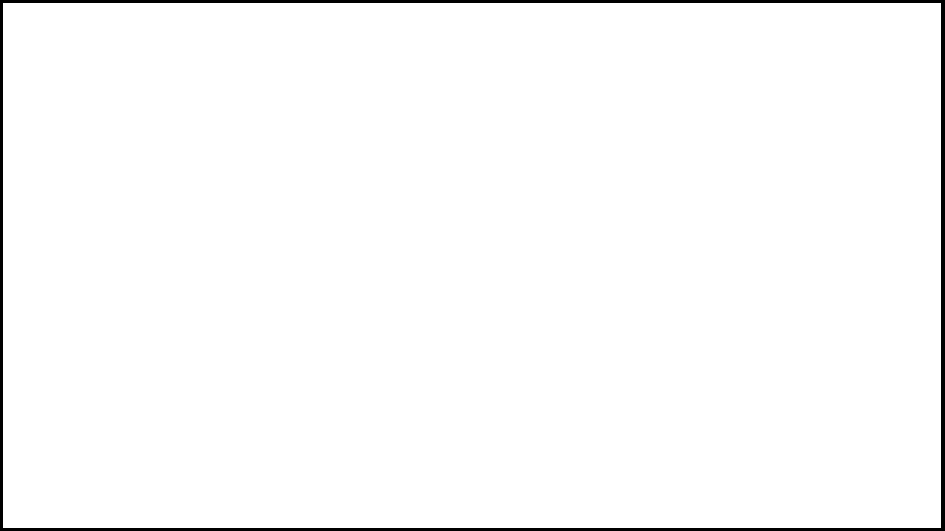
\includegraphics{./croquis/blanc.pdf}

}

\caption{\label{fig-20230302054334}L'application linéaire tangente
\(\tens{F}\) transporte le vecteur matériel \((\D\xi, \D\eta)\) de la
configuration initiale (\(\D\altvec{\point{M}}\)) vers la configuration
actuelle (\(\D\altvec{\point{m}}\)).}

\end{figure}

\hypertarget{duxe9formations-membranaires-de-la-coque}{%
\section{Déformations membranaires de la
coque}\label{duxe9formations-membranaires-de-la-coque}}

Par analogie avec la mécanique des milieux continus, on mesure les
déformations de la coque au cours de sa transformation par la variation
du produit scalaire entre deux vecteurs matériels construits au même
point. En d'autres termes, on considère les trois points matériels
voisins suivants (voir Figure~\ref{fig-20230302055151}) \[
(\xi, \eta), \quad (\xi_1 = \xi + \D \xi_1, \eta_1 = \eta + \D \eta_1)
\quad \text{et} \quad
(\xi_2 = \xi + \D \xi_2, \eta_2 = \eta + \D \eta_2)
\] et on construit les vecteurs matériels \((\D \xi_1, \D \eta_1)\) et
\((\D \xi_2, \D \eta_2)\). En configuration initiale, ces vecteurs
matériels sont représentés par \[
\D\altvec{\point{M}}_1 = \vec{A}_\xi \, \D \xi_1 + \vec{A}_\eta \, \D \eta_1
\quad \text{et} \quad
\D\altvec{\point{M}}_2 = \vec{A}_\xi \, \D \xi_2 + \vec{A}_\eta \, \D \eta_2,
\] tandis que, en configuration actuelle \[
\D\altvec{\point{m}}_1 = \vec{a}_\xi \, \D \xi_1 + \vec{a}_\eta \, \D \eta_1
\quad \text{et} \quad
\D\altvec{\point{m}}_2 = \vec{a}_\xi \, \D \xi_2 + \vec{a}_\eta \, \D \eta_2.
\]

La relation de transport (\ref{eq-20230301171229}) permet alors
d'exprimer la variation du produit scalaire de ces deux vecteurs
matériels \[
\begin{aligned}[b]
\D\altvec{\point{m}}_1 \cdot \D\altvec{\point{m}}_2 - \D\altvec{\point{M}}_1 \cdot \D\altvec{\point{M}}_2
&= \bigl(\tens{F} \cdot \D\altvec{\point{M}}_1 \bigr) \cdot \bigl(\tens{F} \cdot \D\altvec{\point{M}}_2 \bigr) - \D\altvec{\point{M}}_1 \cdot \D\altvec{\point{M}}_2\\
&= \D\altvec{\point{M}}_1 \cdot \tens{F}^\transpose \cdot \tens{F} \cdot \D\altvec{\point{M}}_2 - \D\altvec{\point{M}}_1 \cdot \D\altvec{\point{M}}_2.
\end{aligned}
\]

Le tenseur \(\tens{F}^\transpose \cdot \tens{F}\) est un tenseur
symétrique du plan tangent \(\mathcal{T}(\point{M}, \Sigma)\) (puisque
\(\tens{F} \cdot \vec{N} = \vec{0}\)). Les vecteurs
\(\D\altvec{\point{M}}_1\) et \(\D\altvec{\point{M}}_2\) étant eux-mêmes
des vecteurs de ce plan tangent, on peut écrire \[
\D\altvec{\point{m}}_1 \cdot \D\altvec{\point{m}}_2 - \D\altvec{\point{M}}_1 \cdot \D\altvec{\point{M}}_2 = \D\altvec{\point{M}}_1 \cdot \bigl( \tens{F}^\transpose \cdot \tens{F} - \tens{A} \bigr) \cdot \D\altvec{\point{M}}_2.
\]

On introduit alors le \textbf{tenseur des déformations membranaires}
\begin{equation}\protect\hypertarget{eq-20230301174444}{}{
\tens{E} = \tfrac{1}{2} \bigl( \tens{F}^\transpose \cdot \tens{F} - \tens{A} \bigr),
}\label{eq-20230301174444}\end{equation} de sorte que \[
\D\altvec{\point{M}}_1 \cdot \tens{E} \cdot \D\altvec{\point{M}}_2 = \tfrac{1}{2} \bigl( \D\altvec{\point{m}}_1 \cdot \D\altvec{\point{m}}_2 - \D\altvec{\point{M}}_1 \cdot \D\altvec{\point{M}}_2 \bigr).
\]

\begin{tcolorbox}[enhanced jigsaw, toptitle=1mm, title=\textcolor{quarto-callout-note-color}{\faInfo}\hspace{0.5em}{Note}, colbacktitle=quarto-callout-note-color!10!white, toprule=.15mm, left=2mm, bottomrule=.15mm, arc=.35mm, breakable, opacityback=0, colframe=quarto-callout-note-color-frame, bottomtitle=1mm, titlerule=0mm, leftrule=.75mm, opacitybacktitle=0.6, coltitle=black, rightrule=.15mm, colback=white]

Le tenseur ainsi introduit joue le même rôle que le tenseur de
Green--Lagrange de la mécanique des milieux continus. L'interprétation
de ses coefficients est identique (dans le plan tangent).

\end{tcolorbox}

\begin{figure}

{\centering 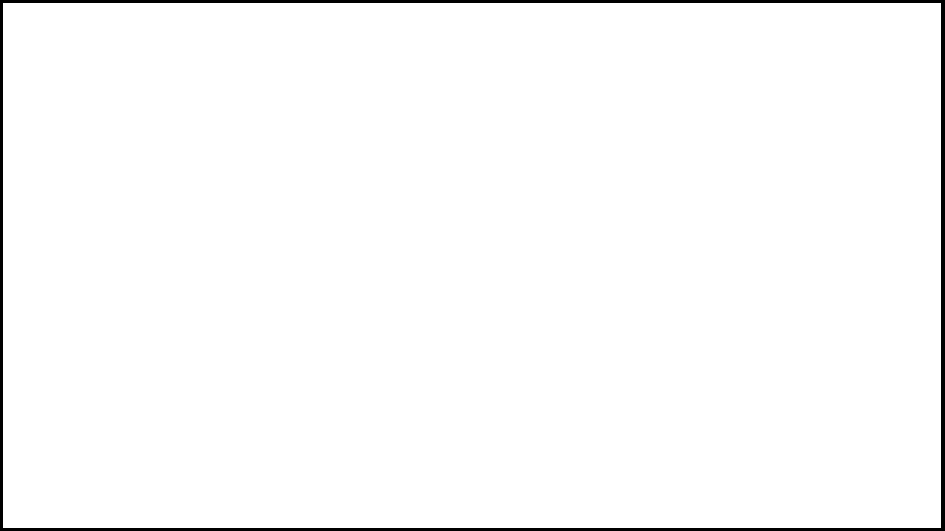
\includegraphics{./croquis/blanc.pdf}

}

\caption{\label{fig-20230302055151}Le transport de deux vecteurs
matériels construits au même point permet de définir le tenseur des
déformations membranaires.}

\end{figure}

\bookmarksetup{startatroot}

\hypertarget{duxe9rivation-et-intuxe9gration-sur-une-surface}{%
\chapter{Dérivation et intégration sur une
surface}\label{duxe9rivation-et-intuxe9gration-sur-une-surface}}

On considère dans ce chapitre une surface \(ς\) et sa représentation
paramétrique \((ξ, η) ∈ \mathcal{D} ⊂ ℝ^2 ↦ \point{f}(ξ, η) ∈ ℝ^3\). La
base locale naturelle \((\vec{a}_ξ, \vec{a}_η)\) et la normale
\(\vec{n}\) ont été introduites au chapitre précédent \[
\vec{a}_ξ(ξ, η) = ∂_ξ \point{f}(ξ, η), \quad \vec{a}_η(ξ, η) = ∂_η \point{f}(ξ, η) \quad \text{et} \quad \vec{n} = \vec{n}(ξ, η) = \frac{\vec{a}_ξ(ξ, η) \wedge \vec{a}_η(ξ, η)}{\lVert \vec{a}_ξ(ξ, η) \wedge \vec{a}_η(ξ, η) \rVert}.
\]

\hypertarget{base-duale-et-notations-de-ricci}{%
\section{Base duale et notations de
Ricci}\label{base-duale-et-notations-de-ricci}}

Dans une base cartésienne otrhonormée
\((\vec{e}_1, \vec{e}_2, \vec{e}_3)\), le produit scalaire avec les
vecteurs de la base permet d'extraire les coordonnées d'un vecteur.
Ainsi, pour tout vecteur \(\vec{v} ∈ ℝ^3\) \[
\vec{v} = \bigl( \vec{v} ⋅ \vec{e}_1 \bigr) \, \vec{e}_2 + \bigl( \vec{v} ⋅ \vec{e}_2 \bigr) \, \vec{e}_2 + \bigl( \vec{v} ⋅ \vec{e}_3 \bigr) \, \vec{e}_3.
\]

La base locale naturelle n'est en général \textbf{ni orthogonale, ni
normée} et \textbf{la relation précédente ne s'applique pas} \[
\vec{v} ≠ \bigl( \vec{v} ⋅ \vec{a}_ξ \bigr) \, \vec{a}_ξ + \bigl( \vec{v} ⋅ \vec{a}_η \bigr) \, \vec{a}_η + \bigl( \vec{v} ⋅ \vec{n} \bigr) \, \vec{n}.
\]

On souhaite construire trois vecteurs \(\vec{a}^ξ\), \(\vec{a}^η\) et
\(\vec{n}^*\) (attention à la position des indices~!), tels que la
relation suivante soit, elle, vraie pour tout \(\vec{v} ∈ ℝ^3\)
\begin{equation}\protect\hypertarget{eq-20230404144735}{}{
\vec{v} = \bigl( \vec{v} ⋅ \vec{a}^ξ \bigr) \, \vec{a}_ξ + \bigl( \vec{v} ⋅ \vec{a}^η \bigr) \, \vec{a}_η + \bigl( \vec{v} ⋅ \vec{n}^* \bigr) \, \vec{n}.
}\label{eq-20230404144735}\end{equation}

Les vecteurs suivants satisfont bien cette relation et on peut vérifier
que ce sont les seuls
\begin{equation}\protect\hypertarget{eq-20230404160223}{}{
\vec{a}^ξ = \frac{ \vec{a}_η \wedge \vec{n} }{ \lVert \vec{a}_ξ \wedge \vec{a}_η \rVert}, \quad
\vec{a}^η = - \frac{ \bigl( \vec{a}_ξ \wedge \vec{n} }{ \lVert \vec{a}_ξ \wedge \vec{a}_η \rVert}
\quad \text{et} \quad \vec{n}^* = \vec{n}.
}\label{eq-20230404160223}\end{equation}

\begin{tcolorbox}[enhanced jigsaw, toptitle=1mm, title=\textcolor{quarto-callout-tip-color}{\faLightbulb}\hspace{0.5em}{Astuce}, colbacktitle=quarto-callout-tip-color!10!white, toprule=.15mm, left=2mm, bottomrule=.15mm, arc=.35mm, breakable, opacityback=0, colframe=quarto-callout-tip-color-frame, bottomtitle=1mm, titlerule=0mm, leftrule=.75mm, opacitybacktitle=0.6, coltitle=black, rightrule=.15mm, colback=white]

\bookmarksetup{startatroot}

\hypertarget{duxe9monstration-6}{%
\chapter{Démonstration}\label{duxe9monstration-6}}

On raisonne par analyse et synthèse, en supposant que les vecteurs
cherchés existent. On écrit alors la relation (\ref{eq-20230404144735})
successivement pour \(\vec{v} = \vec{a}_ξ\), puis
\(\vec{v} = \vec{a}_η\), enfin \(\vec{v} = \vec{n}\). On obtient ainsi
\[
\left\{
\begin{aligned}
\vec{a}_ξ &= \bigl( \vec{a}_ξ ⋅ \vec{a}^ξ \bigr) \, \vec{a}_ξ + \bigl( \vec{a}_ξ ⋅ \vec{a}^η \bigr) \, \vec{a}_η + \bigl( \vec{a}_ξ ⋅ \vec{n}^* \bigr) \, \vec{n},\\
\vec{a}_η &= \bigl( \vec{a}_η ⋅ \vec{a}^ξ \bigr) \, \vec{a}_η + \bigl( \vec{a}_η ⋅ \vec{a}^η \bigr) \, \vec{a}_η + \bigl( \vec{a}_η ⋅ \vec{n}^* \bigr) \, \vec{n},\\
\vec{n} &= \bigl( \vec{n} ⋅ \vec{a}^ξ \bigr) \, \vec{n} + \bigl( \vec{n} ⋅ \vec{a}^η \bigr) \, \vec{a}_η + \bigl( \vec{n} ⋅ \vec{n}^* \bigr) \, \vec{n}
\end{aligned}
\right.
\] et, puisque les vecteurs \(\vec{a}_ξ\), \(\vec{a}_η\) et \(\vec{n}\)
forment une base \[
\begin{aligned}
\vec{a}_ξ ⋅ \vec{a}^ξ &= 1, & \vec{a}_ξ ⋅ \vec{a}^η &= 0, & \vec{a}_ξ ⋅ \vec{n}^* &= 0,\\
\vec{a}_η ⋅ \vec{a}^ξ &= 0, & \vec{a}_η ⋅ \vec{a}^η &= 1, & \vec{a}_η ⋅ \vec{n}^* &= 0,\\
\vec{n}   ⋅ \vec{a}^ξ &= 0, & \vec{n}   ⋅ \vec{a}^η &= 0, & \vec{n}   ⋅ \vec{n}^* &= 1.
\end{aligned}
\]

Ces relations définissent de manière unique les vecteurs \(\vec{a}^ξ\),
\(\vec{a}^η\) et \(\vec{n}^*\) (le vérifier~!). Inversement, on vérifie
que les vecteurs donnés par la relation (\ref{eq-20230404160223})
satisfont bien la relation (\ref{eq-20230404144735}).

\end{tcolorbox}

\begin{tcolorbox}[enhanced jigsaw, toptitle=1mm, title=\textcolor{quarto-callout-warning-color}{\faExclamationTriangle}\hspace{0.5em}{Remarque}, colbacktitle=quarto-callout-warning-color!10!white, toprule=.15mm, left=2mm, bottomrule=.15mm, arc=.35mm, breakable, opacityback=0, colframe=quarto-callout-warning-color-frame, bottomtitle=1mm, titlerule=0mm, leftrule=.75mm, opacitybacktitle=0.6, coltitle=black, rightrule=.15mm, colback=white]

Une démonstration plus générale est possible (en dimension quelconque),
en considérant l'isomorphisme canonique qui existe entre un espace
euclidien et son dual.

\end{tcolorbox}

On peut montrer que les vecteurs \(\vec{a}^1\), \(\vec{a}^2\) et
\(\vec{n}^*\) \textbf{linéairement indépendants} et forment une base,
nommée \textbf{base duale de la base locale naturelle}.

\begin{tcolorbox}[enhanced jigsaw, toptitle=1mm, title=\textcolor{quarto-callout-tip-color}{\faLightbulb}\hspace{0.5em}{Démonstration}, colbacktitle=quarto-callout-tip-color!10!white, toprule=.15mm, left=2mm, bottomrule=.15mm, arc=.35mm, breakable, opacityback=0, colframe=quarto-callout-tip-color-frame, bottomtitle=1mm, titlerule=0mm, leftrule=.75mm, opacitybacktitle=0.6, coltitle=black, rightrule=.15mm, colback=white]

Soit \(V = \Span(\vec{a}^ξ, \vec{a}^η, \vec{a^3}) ⊂ ℝ^3\) le sous-espace
engendré par les vecteurs \(\vec{a}^ξ\), \(\vec{a}^η\) et \(\vec{n}^*\).
On considère \(\vec{v} ∈ V^\perp\), c'est-à-dire que
\(\vec{v} ⋅ \vec{a}^ξ = \vec{v} ⋅ \vec{a}^η = \vec{v} ⋅ \vec{n}^* = \vec{0}\).
En appliquant la relation (\ref{eq-20230404144735}), supposée vraie, on
trouve que nécessairement \(\vec{v} = \vec{0}\). L'orthogonal de \(V\)
est donc réduit au vecteur-nul, c'est-à-dire que \(V = ℝ^3\). Donc \(V\)
est de dimension 3~; comme par construction, \(V\) est engendré par
trois vecteurs, ceux-ci sont linéairement indépendants.

\end{tcolorbox}

La relation (\ref{eq-20230404144735}) permet également d'obtenir la
relation symétrique suivante, vraie pour tout \(\vec{v} ∈ ℝ^3\)
\begin{equation}\protect\hypertarget{eq-20230404154755}{}{
\vec{v} = \bigl( \vec{v} ⋅ \vec{a}_ξ \bigr) \, \vec{a}^ξ + \bigl( \vec{v} ⋅ \vec{a}_η \bigr) \, \vec{a}^η + \bigl( \vec{v} ⋅ \vec{n} \bigr) \, \vec{n}^*.
}\label{eq-20230404154755}\end{equation}

\begin{tcolorbox}[enhanced jigsaw, toptitle=1mm, title=\textcolor{quarto-callout-tip-color}{\faLightbulb}\hspace{0.5em}{Démonstration}, colbacktitle=quarto-callout-tip-color!10!white, toprule=.15mm, left=2mm, bottomrule=.15mm, arc=.35mm, breakable, opacityback=0, colframe=quarto-callout-tip-color-frame, bottomtitle=1mm, titlerule=0mm, leftrule=.75mm, opacitybacktitle=0.6, coltitle=black, rightrule=.15mm, colback=white]

Soient \(\vec{v} ∈ ℝ^3\) quelconques, et
\(\tilde{\vec{v}} = ( \vec{v} ⋅ \vec{a}_ξ ) \, \vec{a}^ξ + ( \vec{v} ⋅ \vec{a}_η ) \, \vec{a}^η + ( \vec{v} ⋅ \vec{n} ) \, \vec{n}^*\).
On souhaite montrer que \(\tilde{\vec{v}} = \vec{v}\). Il suffit de
montrer que \(\tilde{\vec{v}} ⋅ \vec{w} = \vec{v} ⋅ \vec{w}\) pour tout
\(\vec{w} ∈ ℝ^3\). L'identité (\ref{eq-20230404144735}) s'écrit, pour
\(\vec{w}\) arbitraire \[
\vec{w} = \bigl( \vec{w} ⋅ \vec{a}^ξ \bigr) \, \vec{a}_ξ + \bigl( \vec{w} ⋅ \vec{a}^η \bigr) \, \vec{a}_η + \bigl( \vec{w} ⋅ \vec{n}^* \bigr) \, \vec{n},
\] soit, en prenant le produit scalaire avec \(\vec{v}\) \[
\begin{aligned}
\vec{w} ⋅ \vec{v} &= \bigl( \vec{w} ⋅ \vec{a}^ξ \bigr) \, \bigl( \vec{v} ⋅ \vec{a}_ξ \bigr) + \bigl( \vec{w} ⋅ \vec{a}^η \bigr) \, \bigl( \vec{v} ⋅ \vec{a}_η \bigr) + \bigl( \vec{w} ⋅ \vec{n}^* \bigr) \, \bigl( \vec{v} ⋅ \vec{n} \bigr)\\
&= \bigl( \vec{w} ⋅ \vec{a}^ξ \bigr) \, \bigl( \vec{v} ⋅ \vec{a}_ξ \bigr) + \bigl( \vec{w} ⋅ \vec{a}^η \bigr) \, \bigl( \vec{v} ⋅ \vec{a}_η \bigr) + \bigl( \vec{w} ⋅ \vec{n}^* \bigr) \, \bigl( \vec{v} ⋅ \vec{n} \bigr)\\
&= \vec{w} ⋅ \bigl[ \bigl( \vec{v} ⋅ \vec{a}_ξ \bigr) \, \vec{a}^ξ + \bigl( \vec{v} ⋅ \vec{a}_η \bigr) \, \vec{a}^η + \bigl( \vec{v} ⋅ \vec{n} \bigr) \, \vec{n}^* \bigr]\\
&= \vec{w} ⋅ \tilde{\vec{v}} \qquad \text{CQFD.}
\end{aligned}
\]

\end{tcolorbox}

On déduit des relations (\ref{eq-20230404144735}) et
(\ref{eq-20230404154755}) que \[
\tens{I} = \vec{a}^ξ ⊗ \vec{a}_ξ + \vec{a}^η ⊗ \vec{a}_η + \vec{n} ⊗ \vec{n} = \vec{a}_ξ ⊗ \vec{a}^ξ + \vec{a}_η ⊗ \vec{a}^η + \vec{n} ⊗ \vec{n},
\] soit \begin{equation}\protect\hypertarget{eq-20230302062218}{}{
\tens{a} = \tens{I} - \vec{n} ⊗ \vec{n} = \vec{a}^ξ ⊗ \vec{a}_ξ + \vec{a}^η ⊗ \vec{a}_η = \vec{a}_ξ ⊗ \vec{a}^ξ + \vec{a}_η ⊗ \vec{a}^η,
}\label{eq-20230302062218}\end{equation}

En convenant dans le reste de ce livre que les indices muets grecs
(\(α\), \(β\), \ldots) parcourent l'ensemble \(\{ξ, η\}\), les relations
(\ref{eq-20230302062218}) s'écrivent \[
\tens{a} = \sum_α \vec{a}^α ⊗ \vec{a}_α = \sum_α \vec{a}_α ⊗ \vec{a}^α.
\]

Dans l'expression ci-dessus, on s'aperçoit que l'indice muet \(α\)
apparaît \textbf{exactement deux fois}, et dans des \textbf{positions
différentes}~: une fois en position inférieure, une fois en position
supérieure. \textbf{Lorsque ces deux conditions sont remplies}, et
uniquement dans ce cas, on pourra utiliser la convention de sommation
d'Einstein \[
\tens{a} = \vec{a}^α ⊗ \vec{a}_α = \vec{a}_α ⊗ \vec{a}^α.
\]

\begin{tcolorbox}[enhanced jigsaw, toptitle=1mm, title=\textcolor{quarto-callout-warning-color}{\faExclamationTriangle}\hspace{0.5em}{Remarque importante}, colbacktitle=quarto-callout-warning-color!10!white, toprule=.15mm, left=2mm, bottomrule=.15mm, arc=.35mm, breakable, opacityback=0, colframe=quarto-callout-warning-color-frame, bottomtitle=1mm, titlerule=0mm, leftrule=.75mm, opacitybacktitle=0.6, coltitle=black, rightrule=.15mm, colback=white]

Il est important de ne jamais sommer sur deux indices répétés dans la
même position (on parle d'indices de \textbf{même variance}). Ainsi, les
expressions \(\vec{a}_α ⊗ \vec{a}_α\) et \(\vec{a}^α ⊗ \vec{a}^α\) n'ont
pas de sens, car elles ne sont \textbf{pas invariantes par changement de
base}. Plus précisément, soient \((\vec{a}_ξ', \vec{a}_η')\) une autre
base du plan tangent et \((\vec{a}'^ξ, \vec{a}'^η)\) la base duale
associée. Alors, en général \[
\vec{a}_ξ ⊗ \vec{a}_ξ + \vec{a}_η ⊗ \vec{a}_η ≠ \vec{a}'_ξ ⊗ \vec{a}'_ξ + \vec{a}'_η ⊗ \vec{a}'_η
\quad \text{et} \quad
\vec{a}^ξ ⊗ \vec{a}^ξ + \vec{a}^η ⊗ \vec{a}^η ≠ \vec{a}'^ξ ⊗ \vec{a}'^ξ + \vec{a}'^η ⊗ \vec{a}'^η
\]

\end{tcolorbox}

\begin{tcolorbox}[enhanced jigsaw, toptitle=1mm, title=\textcolor{quarto-callout-warning-color}{\faExclamationTriangle}\hspace{0.5em}{À faire}, colbacktitle=quarto-callout-warning-color!10!white, toprule=.15mm, left=2mm, bottomrule=.15mm, arc=.35mm, breakable, opacityback=0, colframe=quarto-callout-warning-color-frame, bottomtitle=1mm, titlerule=0mm, leftrule=.75mm, opacitybacktitle=0.6, coltitle=black, rightrule=.15mm, colback=white]

Expression du tenseur antisymétrique fondamental ?

\end{tcolorbox}

\hypertarget{gradient-dun-champ-de-tenseurs}{%
\section{Gradient d'un champ de
tenseurs}\label{gradient-dun-champ-de-tenseurs}}

Soient \(\point{m} = \point{f}(ξ, η)\) et
\(\point{m'} = \point{f}(ξ + \D ξ, η + \D η)\) deux points infiniment
proches de la surface \(ς\), de sorte que \[
\begin{aligned}[b]
\D \altvec{\point{m}}
&= \altvec{\point{mm}'} = \point{m}' - \point{m} = \point{f}(ξ + \D ξ, η + \D η) - \point{f}(ξ, η)\\
&= ∂_ξ \point{f}(ξ, η) \, \D ξ + ∂_η \point{f}(ξ, η) \, \D η.
\end{aligned}
\]

En reconnaissant les vecteurs de la base locale naturelle, et en
utilisant la relation (\ref{eq-20230404144735}), on obtient donc
\begin{equation}\protect\hypertarget{eq-20230404183949}{}{
\D \altvec{\point{m}} = \vec{a}_ξ \, \D ξ + \vec{a}_η \, \D η, \quad \text{soit} \quad \D ξ = \vec{a}^ξ ⋅ \D \altvec{\point{m}} \quad \text{et} \quad \D η = \vec{a}^η ⋅ \D \altvec{\point{m}}
}\label{eq-20230404183949}\end{equation}

Soit alors \(\tens{T}(\point{m})\) un champ de tenseurs d'ordre
quelconque, défini sur la surface \(ς\). En composant par la
représentation paramétrique \(\point{f}\) de la surface, on définit une
application \((ξ, η) ↦ \tens{T} \circ \point{f}(ξ, η)\) définie sur
l'espace des paramètres \(\mathcal{D}\). On souhaite évaluer la
variation \(\D \tens{T}\) du champ \(\tens{T}\) entre les points
\(\point{m}\) et \(\point{m}' = \point{m} + \D \altvec{\point{m}}\) \[
\begin{aligned}[b]
\D \tens{T} &= \tens{T}(\point{m} + \D\altvec{\point{m}}) - \tens{T}(\point{m}) = \tens{T} \circ \point{f}(ξ + \D ξ, η + \D η) - \tens{T} \circ \point{f}(ξ, η)\\
&= ∂_ξ \bigl( \tens{T} \circ \point{f} \bigr) \, \D ξ + ∂_η \bigl( \tens{T} \circ \point{f} \bigr) \, \D η,
\end{aligned}
\] soit, en utilisant les relations (\ref{eq-20230404183949}) \[
\D \tens{T} = ∂_ξ \bigl( \tens{T} \circ \point{f} \bigr) \, \bigl( \vec{a}^ξ ⋅ \D \altvec{\point{m}} \bigr) + ∂_η \bigl( \tens{T} \circ \point{f} \bigr) \, \bigl( \vec{a}^η ⋅ \D \altvec{\point{m}} \bigr) = \tilde{\tens{G}}(ξ, η) ⋅ \D \altvec{\point{m}},
\] en posant \[
\tilde{\tens{G}} = ∂_ξ \bigl( \tens{T} \circ \point{f} \bigr) ⊗ \vec{a}^ξ + ∂_η \bigl( \tens{T} \circ \point{f} \bigr) ⊗ \vec{a}^η,
\] où on remarque que l'application \((ξ, η) ↦ \tilde{\tens{G}}\) est
\textbf{définie sur l'espace des paramètres \(\mathcal{D}\)}. On définit
alors le champ de tenseurs \(\tens{G}\) sur \(ς\) de la façon suivante
\[
\tens{G} = \tilde{\tens{G}} \circ \point{f}^{-1} \quad \text{soit} \quad \tens{G}(\point{m}) = \tilde{\tens{G}}(ξ, η) \quad \text{pour} \quad \point{m} = \point{f}(ξ, η).
\]

On a ainsi mis la variation \(\D \tens{T}\) sous la forme intrinsèque
suivante \[
\D \tens{T} = \tens{T}(\point{m} + \D \altvec{\point{m}}) - \tens{T}(\point{m}) = \tens{G}(\point{m}) ⋅ \D \altvec{\point{m}}.\]

On reconnaît la définition usuelle d'un gradient\textasciitilde: le
champ \(\tens{G}\) ainsi défini est le \textbf{gradient surfacique} de
\(\tens{T}\) ; on le note \(\tgrad\tens{T}\) \[
\tgrad \tens{T}(\point{m}) = ∂_ξ \bigl( \tens{T} \circ \point{f} \bigr) ⊗ \vec{a}^ξ + ∂_η \bigl( \tens{T} \circ \point{f} \bigr) ⊗ \vec{a}^η
\quad \text{avec},
\] où \(\vec{a}^ξ\), \(\vec{a}^η\), \(\tens{T} \circ \point{f}\) et ses
dérivées sont implicitement évalués en \((ξ, η)\) tels que
\(\point{f}(ξ, η) = \point{m}\). Si \(\tens{T}\) est un champ de
tenseurs d'ordre \(n\), alors \(\tgrad \tens{T}\) est un champ de
tenseurs d'ordre \(n + 1\). On a de plus toujours, par construction \[
\tgrad{\tens{T}} ⋅ \vec{n} = \tens{0}.
\]

\begin{tcolorbox}[enhanced jigsaw, toptitle=1mm, title=\textcolor{quarto-callout-note-color}{\faInfo}\hspace{0.5em}{Remarque}, colbacktitle=quarto-callout-note-color!10!white, toprule=.15mm, left=2mm, bottomrule=.15mm, arc=.35mm, breakable, opacityback=0, colframe=quarto-callout-note-color-frame, bottomtitle=1mm, titlerule=0mm, leftrule=.75mm, opacitybacktitle=0.6, coltitle=black, rightrule=.15mm, colback=white]

La définition précédente du gradient fait intervenir un paramétrage
particulier \((ξ, η) ↦ \point{f}(ξ, η)\) de la surface. Pour autant, le
champ \(\tgrad \tens{T}\) ainsi construit est bien intrinsèque. Ainsi,
on peut vérifier que si \((φ, ψ) ↦ \point{g}(φ, ψ)\) désigne un second
paramétrage de la surface, alors \[
∂_ξ \bigl( \tens{T} \circ \point{f} \bigr) ⊗ \vec{a}^ξ + ∂_η \bigl( \tens{T} \circ \point{f} \bigr) ⊗ \vec{a}^η
= ∂_φ \bigl( \tens{T} \circ \point{g} \bigr) ⊗ \vec{a}^φ + ∂_ψ \bigl( \tens{T} \circ \point{g} \bigr) ⊗ \vec{a}^ψ,
\] où \(\vec{a}^ξ\), \(\vec{a}^η\), \(\tens{T} \circ \point{f}\) et ses
dérivées sont implicitement évalués en \((ξ, η)\), tandis que
\(\vec{a}^φ\), \(\vec{a}^ψ\), \(\tens{T} \circ \point{g}\) et ses
dérivées sont implicitement évalués en \((φ, ψ)\) tels que
\(\point{f}(ξ, η) = \point{g}(φ, ψ) = \point{m}\).

\end{tcolorbox}

L'opérateur gradient ainsi défini est un \textbf{opérateur linéaire}
dont les propriétés sont proches de celles du gradient usuel. On peut
également définir la \textbf{divergence surfacique} d'un champ de
tenseurs \(\tens{T}\) d'ordre \(n ≥ 1\) \[
\tdiv \tens{T} = \tgrad \tens{T} \dbldot \tens{a},
\] c'est un champ de tenseurs d'ordre \(n - 1\).

\begin{tcolorbox}[enhanced jigsaw, toptitle=1mm, title=\textcolor{quarto-callout-warning-color}{\faExclamationTriangle}\hspace{0.5em}{Remarque importante}, colbacktitle=quarto-callout-warning-color!10!white, toprule=.15mm, left=2mm, bottomrule=.15mm, arc=.35mm, breakable, opacityback=0, colframe=quarto-callout-warning-color-frame, bottomtitle=1mm, titlerule=0mm, leftrule=.75mm, opacitybacktitle=0.6, coltitle=black, rightrule=.15mm, colback=white]

Les développements précédents permettent d'assurer que la définition du
gradient proposée est intrinsèque. En pratique néanmoins, il sera
commode de travailler directement avec le champ surfacique
\(\tens{T} \circ \point{f}\) qui est alors une fonction des fonctions
des paramètres \(ξ\) et \(η\) (plutôt que comme une fonction du point
\(\point{m} ∈ ς\)). Par abus de langage, on écrira, comme c'est
l'habitude, \(\tens{T}(ξ, η)\) plutôt que
\(\tens{T} \circ \point{f}(ξ, η)\). En revanche, on écrira explicitement
\(∂_α\tens{T} ⊗ \vec{a}^α\) et \(∂_α\tens{T} ⋅ \vec{a}^α\) plutôt que
\(\tgrad \tens{T}\) et \(\tdiv \tens{T}\) (noter l'utilisation de la
convention d'Einstein, possible car l'indice \(α\) apparaît une fois en
position inférieure et une fois en position supérieure).

\end{tcolorbox}

\begin{tcolorbox}[enhanced jigsaw, toptitle=1mm, title=\textcolor{quarto-callout-warning-color}{\faExclamationTriangle}\hspace{0.5em}{À faire}, colbacktitle=quarto-callout-warning-color!10!white, toprule=.15mm, left=2mm, bottomrule=.15mm, arc=.35mm, breakable, opacityback=0, colframe=quarto-callout-warning-color-frame, bottomtitle=1mm, titlerule=0mm, leftrule=.75mm, opacitybacktitle=0.6, coltitle=black, rightrule=.15mm, colback=white]

Proposer les propriétés du gradient en exercice.

\end{tcolorbox}

\hypertarget{lien-avec-la-courbure}{%
\section{Lien avec la courbure}\label{lien-avec-la-courbure}}

\begin{tcolorbox}[enhanced jigsaw, toptitle=1mm, title=\textcolor{quarto-callout-warning-color}{\faExclamationTriangle}\hspace{0.5em}{À faire}, colbacktitle=quarto-callout-warning-color!10!white, toprule=.15mm, left=2mm, bottomrule=.15mm, arc=.35mm, breakable, opacityback=0, colframe=quarto-callout-warning-color-frame, bottomtitle=1mm, titlerule=0mm, leftrule=.75mm, opacitybacktitle=0.6, coltitle=black, rightrule=.15mm, colback=white]

\end{tcolorbox}

\bookmarksetup{startatroot}

\hypertarget{sec-20230328142259}{%
\chapter{Membranes}\label{sec-20230328142259}}

On établit dans ce chapitre la théorie des \textbf{membranes},
c'est-à-dire des coques sans raideur à la flexion. On fait l'hypothèse
que l'état de contraintes des membranes est complètement défini par la
mesure des \textbf{déformations membranaires} introduites au chapitre
Chapitre~\ref{sec-20230314085944}.

\bookmarksetup{startatroot}

\hypertarget{coques-en-uxe9quilibre-membranaire}{%
\chapter{Coques en équilibre
membranaire}\label{coques-en-uxe9quilibre-membranaire}}

Le présent chapitre est consacré aux coques en équilibre membranaire.
Comme les membranes, ce sont des systèmes mécaniques qui équilibrent
leur chargement par des \textbf{efforts membranaires seulement} (pas de
moments fléchissants). Contrairement aux membranes, la raideur en
flexion des coques en équilibre membranaire est suffisante pour leur
permettre d'équilibrer les chargements \textbf{sans changer de
géométrie}. La théorie des coques en équilibre membranaire est donc
formulée dans \textbf{l'hypothèse des petites perturbations}.

Cette théorie peut être vue comme une approche en contraintes
(généralisées) de l'équilibre des coques élastiques. La géométrie de la
coque et son chargement étant donnés, on verra en effet qu'il est en
général toujours possible de construire un champ de contraintes
généralisées purement membranaires et statiquement admissibles avec le
chargement. Comme dans l'approche en contraintes de l'équilibre
élastique des milieux continus, il s'agit alors d'intégrer le champ des
déformations (généralisées) pour remonter aux déplacements
(généralisés). Cette dernière étape n'est pas toujours possible~: dans
ce cas, l'hypothèse d'équilibre \textbf{membranaire} de la coque est
mise en défaut, et on doit traiter un problème général dans lequel
efforts membranaires et flexion sont couplés.

Bien qu'elle ne soit pas toujours vérifiée, il est fréquent en phase
initiale d'un projet de faire l'hypothèse d'un équilibre membranaire,
qui permet d'estimer aisément les efforts intérieurs et d'obtenir ainsi
un prédimensionnement. Il convient ensuite de vérifier que cette
hypothèse est valide. Dans un grand nombre de situations pratiques, on
constate que cette hypothèse n'est violée que \textbf{localement}~: dans
les phases suivantes du projet, la coque est alors renforcée dans ces
zones uniquement afin de reprendre les efforts de flexion qui s'y
développent.

Dans ce chapitre, on présente les équations des coques en équilibre
membranaires, ainsi que quelques exemples d'application.

On rappelle que la théorie des coques en équilibre membranaire est
formulée dans le cadre de l'hypothèse des petites perturbations. Il n'y
a donc pas lieu de distinguer les configurations initiale \(\Sigma\) et
actuelle \(\varsigma\) (toutes deux désignées par \(\Sigma\) dans ce qui
suit), ni les contraintes généralisées \(\tens{N}^\KL\) et
\(\tens{N}^\kl\) (toutes deux désignées par \(\tens{N}\) dans ce qui
suit). De même, on ne distingue pas les opérateurs différentiels
\(\Div\) et \(\div\), \(\Grad\) et \(\grad\).

\hypertarget{uxe9quilibre-membranaire-des-coques}{%
\section{Équilibre membranaire des
coques}\label{uxe9quilibre-membranaire-des-coques}}

Dans l'hypothèse d'un équilibre membranaire, les équations d'équilibre
d'une coque ont été établies au chapitre précédent sur la configuration
\textbf{actuelle}. Puisqu'on confond ici configurations initiale et
actuelle, ces équations d'équilibre s'écrivent simplement
\begin{equation}\protect\hypertarget{eq-20230320105306}{}{
\div \tens{N} + \vec{p} = \vec{0},
}\label{eq-20230320105306}\end{equation} où \(\vec{p}\) désigne la
densité surfacique de forces (par unité de surface de la coque). Le
tenseur \(\tens{N}\) est le tenseur des efforts membranaires~; c'est un
tenseur symétrique du plan tangent, dont on rappelle l'interprétation
physique.

\begin{tcolorbox}[enhanced jigsaw, toptitle=1mm, title=\textcolor{quarto-callout-warning-color}{\faExclamationTriangle}\hspace{0.5em}{Interprétation physique des contraintes membranaires}, colbacktitle=quarto-callout-warning-color!10!white, toprule=.15mm, left=2mm, bottomrule=.15mm, arc=.35mm, breakable, opacityback=0, colframe=quarto-callout-warning-color-frame, bottomtitle=1mm, titlerule=0mm, leftrule=.75mm, opacitybacktitle=0.6, coltitle=black, rightrule=.15mm, colback=white]

La résultante des efforts intérieurs exercés sur la facette \(\D s\) de
normale unitaire \(\vec{g}\) est \[
\D \vec{R}_\internal = \tens{N} \cdot \vec{g} \, \D s.
\]

\end{tcolorbox}

À l'équation d'équilibre précédente, il faut joindre la condition aux
limites sur \(\partial \Sigma\) \[
\tens{N} \cdot \vec{g} = \vec{q},
\] où \(\vec{g}\) désigne la normale unitaire \textbf{sortante} au bord
\(\partial \Sigma\) et \(\vec{q}\) est la densité linéique des forces
exercées sur ce bord.

On rappelle que

\begin{enumerate}
\def\labelenumi{\arabic{enumi}.}
\tightlist
\item
  Les forces exercées au bord de la coque sont nécessairement contenues
  dans le plan tangent.
\item
  Un point régulier de la coque ne peut équilibrer une force ponctuelle.
\end{enumerate}

La projection selon la normale \(\vec{n}\) de l'équation aux dérivées
partielles (\ref{eq-20230320105306}) conduit à une équation algébrique,
dite \textbf{équation d'équilibre normal} \[
\tens{b} \dbldot \tens{N} + \vec{p} \cdot \vec{n} = 0,
\] où \(\tens{b}\) est le tenseur de courbure de la coque.

En résumé, l'équilibre membranaire d'une coque se met en équation de la
façon suivante

\begin{equation}\protect\hypertarget{eq-20230320112037}{}{
\tens{a} \cdot \div \tens{N} + \tens{a} \cdot \vec{p} = \vec{0} \qquad (\Sigma),
}\label{eq-20230320112037}\end{equation}
\begin{equation}\protect\hypertarget{eq-20230320112043}{}{
\tens{b} \dbldot \tens{N} + \vec{p} \cdot \vec{n} = 0 \qquad (\Sigma),
}\label{eq-20230320112043}\end{equation}
\begin{equation}\protect\hypertarget{eq-20230320112048}{}{
\tens{N} \cdot \vec{g} = \vec{q} \qquad (\partial \Sigma).
}\label{eq-20230320112048}\end{equation}

En général, la géométrie \(\Sigma\) de la coque et son chargement
\(\vec{p}\) étant fixés, il est toujours possible de trouver une
solution au système précédent. Par ailleurs, on évite lorsque c'est
possible de résoudre l'équation aux dérivées partielles
(\ref{eq-20230320112037}) en écrivant plutôt l'équilibre de
sous-systèmes bien choisis.

\hypertarget{uxe9quilibre-membranaire-des-coques-axisymuxe9triques}{%
\section{Équilibre membranaire des coques
axisymétriques}\label{uxe9quilibre-membranaire-des-coques-axisymuxe9triques}}

On considère la coque axisymétrique dont la génératrice est représentée
ci-après (voir Figure~\ref{fig-20230320112648}). On rappelle
l'expression du tenseur des courbures \[
\tens{b} = b_{tt} \, \vec{t} \otimes \vec{t} - \frac{\cos \psi}{r} \, \vec{e}_\theta \otimes \vec{e}_\theta,
\] où \(b_{tt}\) désigne la courbure de la génératrice (vue comme une
courbe plane). On suppose que les chargements surfacique \(\vec{p}\) et
linéique \(\vec{q}\) sont axisymétriques et n'ont pas de composante
orthoradiale \[
\vec{p} = p_t(s) \, \vec{t} + p_n(s) \, \vec{n} \quad \text{et} \quad
\vec{q} = q_t \, \vec{t}
\] où les composantes \(p_t\) et \(p_n\) et \(q_t\) ne dépendent pas de
l'angle \(\theta\).

\begin{figure}

{\centering 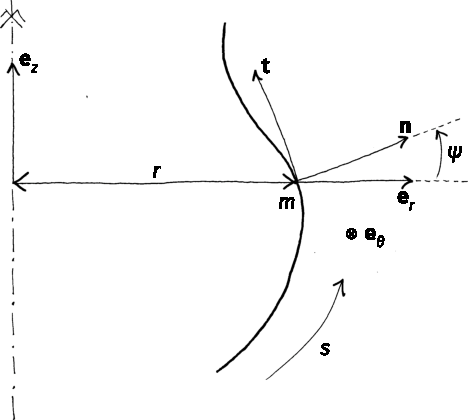
\includegraphics{./croquis/fig20230307165827.pdf}

}

\caption{\label{fig-20230320112648}Génératrice de la coque axisymétrique
considérée.}

\end{figure}

Soit \(\Pi\) un plan horizontal à l'altitude \(z\) fixée. On considère
le sous-système \(\Sigma'\) constitué par la partie de la coque située
\textbf{au-dessus} du plan \(\Pi\). Les moments étant évalués par
rapport à un point de l'axe de révolution, on s'intéresse au torseur des
efforts extérieurs (résultante~: \(\vec{R}_\external'\)~; moment~:
\(\vec{M}_\external'\)) et intérieurs (résultante~:
\(\vec{R}_\internal'\)~; moment~: \(\vec{M}_\internal'\)) exercés sur ce
sous-système. L'équilibre du sous-système considéré conduit à \[
\vec{R}_\internal' + \vec{R}_\external' = \vec{0}
\quad \text{et} \quad
\vec{M}_\internal' + \vec{M}_\external' = \vec{0}.
\]

Compte-tenu de l'invariance par rotation autour de l'axe vertical de la
géométrie et du chargement, la composante verticale
\(\vec{M}_\external' \cdot \vec{e}_z\) du moment des actions extérieures
est nul \[
\vec{M}_\external' \cdot \vec{e}_z = \vec{M}_\internal' \cdot \vec{e}_z = 0.
\]

Les efforts intérieurs s'exercent au droit de la coupure~; la normale
sortante étant \(-\vec{t}\), la densité linéique des efforts extérieurs
est \(-\tens{N} \cdot \vec{t}\). Si \(r\) désigne le rayon du parallèle
contenu dans le plan \(\Pi\), le moment des efforts intérieurs s'écrit
\[
\vec{M}_\internal' = \int_0^{2\pi} \bigl(r \, \vec{e}_r + z \, \vec{e}_z \bigr) \wedge \bigl( -\tens{N} \cdot \vec{t} \bigr) \, r \, \D \theta,
\] soit \[
\vec{M}_\internal' \cdot \vec{e}_z = -\int_0^{2\pi} r^2 \, \bigl( \vec{t} \cdot \tens{N} \cdot \vec{e}_\theta \bigr) \, \D \theta = -2\pi \, r^2 \, \bigl( \vec{t} \cdot \tens{N} \cdot \vec{e}_\theta \bigr),
\] où l'on remarque que l'effort membranaire
\(\bigl( \vec{t} \cdot \tens{N} \cdot \vec{e}_\theta \bigr)\) est
indépendant de \(\theta\). On en déduit finalement que \[
\vec{t} \cdot \tens{N} \cdot \vec{e}_\theta = 0
\] (pas de cisaillements plans). Il reste donc à déterminer les
composantes \(N_{tt}\) et \(N_{\theta\theta}\) du tenseur des efforts
membranaires.

Pour déterminer \(N_{tt}\), il suffit d'écrire l'équilibre en résultante
selon la verticale du sous-système \(\Sigma'\) considéré. En effet \[
\vec{R}_\internal' = \int_{0}^{2\pi} \bigl( -\tens{N} \cdot \vec{t} \bigr) \, r \, \D \theta = -r \, N_{tt} \int_{0}^{2\pi} \vec{t} \, \D \theta = -2\pi \, r \, \cos \psi \, N_{tt} \, \vec{e}_z,
\] soit \[
N_{tt} = \frac{\vec{R}_\external' \cdot \vec{e}_z}{2\pi \, r \, \cos \psi}.
\]

La résultante \(\vec{R}_\external'\) dépend de l'application et doit
être évaluée au cas par cas. On en déduit alors l'expression de
\(N_{tt}\) par la relation précédente. Finalement, on utilise l'équation
d'équilibre normal (\ref{eq-20230320112043}) pour déterminer
\(N_{\theta\theta}\) \[
N_{\theta\theta} = \frac{r}{\cos \psi} \bigl( b_{tt} \, N_{tt} + \vec{p} \cdot \vec{n} \bigr).
\]

\hypertarget{duxe9formations-des-coques-en-uxe9quilibre-membranaire}{%
\section{Déformations des coques en équilibre
membranaire}\label{duxe9formations-des-coques-en-uxe9quilibre-membranaire}}

Dans l'hypothèse des petites perturbations, on peut linéariser
l'expression des déformations membranaires en fonction du champ des
déplacements \[
\tens{E} \simeq \tens{\varepsilon} = \sym \bigl( \tens{a} \cdot \grad \vec{u} \bigr).
\]

Afin de déterminer les déplacements, il faut relier les déformations
membranaires aux efforts membranaires par l'intermédiaire des
\textbf{relations de comportement}. Celles-ci ne peuvent être obtenues
que par une analyse de la coque vue comme un solide tridimensionnel.
Nous admettrons ici que, pour une coque linéairement élastique \[
\tens{N} = \frac{E \, h}{1 - \nu^2} \bigl[ \bigl( 1 - \nu \bigr) \tens{\varepsilon} + \nu \, \bigl( \tr \tens{\varepsilon} \bigr) \, \tens{a} \bigr],
\] où \(h\) désigne l'épaisseur de la coque, \(E\) son module d'Young et
\(\nu\) son coefficient de Poisson. Dans une base orthonormée
\((\vec{e}_1, \vec{e}_2)\) du plan tangent, les relations de
comportement s'écrivent \[
N_{11} = \frac{E \, h}{1 - \nu^2} \bigl( \varepsilon_{11} + \nu \, \varepsilon_{22} \bigr), \quad N_{22} = \frac{E \, h}{1 - \nu^2} \bigl( \varepsilon_{22} + \nu \, \varepsilon_{11} \bigr),
\] \[
N_{12} = \frac{E \, h}{1 + \nu} \, \varepsilon_{12}.
\]

Ces relations s'inversent comme suit \[
\varepsilon_{11} = \frac{N_{11} - \nu \, N_{22}}{E \, h}, \quad \varepsilon_{22} = \frac{N_{22} - \nu \, N_{11}}{E \, h} \quad \text{et} \quad \varepsilon_{12} = \frac{1 + \nu}{E \, h} \, N_{12}.
\]

Une fois déterminés les efforts membranaires, on peut alors établir
l'expression des déformations membranaires linéarisées. Si celles-ci
sont \textbf{géométriquement compatibles}, les déplacements sont alors
obtenus par intégration. Dans le cas contraire, l'hypothèse d'équilibre
membranaire n'était pas légitime et il est nécessaire de prendre en
compte la \textbf{flexion} dans la coque.

\bookmarksetup{startatroot}

\hypertarget{sec-20230411093311}{%
\chapter{Coques en flexion}\label{sec-20230411093311}}

Dans ce chapitre, on présente le modèle de Kirchhoff--Love. C'est le
modèle de coques le plus simple qui permette de rendre compte de
couplages membrane-flexion. Le modèle de membrane a été formulé au
Chapitre~\ref{sec-20230328142259} sous les hypothèses suivantes~: (1)
seuls les degrés de liberté de translation des points de la coque
interviennent dans l'expression de la puissance des efforts extérieurs
et (2) la puissance des efforts intérieurs est une forme linéaire du
seul tenseur des déformations membranaires. Ces hypothèses très
restrictives conduisent à un modèle qui n'a pas de raideur en flexion.
On lève successivement ces deux hypothèses dans le présent chapitre,
organisé comme suit. L'hypothèse de Kirchhoff--Love est introduite au
§~\ref{sec-20230330121445}. Cette hypothèse permet de définir une
rotation sans introduire de degrés de libertés supplémentaires, et donc
de prendre en compte des moments extérieurs. On introduit ensuite au
paragraphe §~\ref{sec-20230328153349} le tenseur des variations des
courbures, qui complète le tenseur des déformations membranaires~: à eux
deux, ils caractérisent les mouvements de corps rigides. Le modèle de
Kirchhoff--Love est construit par la méthode des puissances virtuelles
au §~\ref{sec-20230330121852}. Il est complété au
§~\ref{sec-20230330135827} par les relations de comportement pour un
matériau constitutif de Kirchhoff--Saint-Venant. Finalement, une
synthèse des équations du modèle est présentée au
§~\ref{sec-20230330140022}.

\hypertarget{sec-20230330121445}{%
\section{L'hypothèse de Kirchhoff--Love}\label{sec-20230330121445}}

Dans le modèle de Kirchhoff--Love, les points matériels n'ont par
construction que \textbf{trois degrés de liberté} de translation. Afin
de rendre compte de phénomènes de flexion dans la coque, il est
nécessaire de faire travailler les moments contre une \textbf{rotation}.
Celle-ci est nécessairement \textbf{liée à la translation}, afin de ne
pas introduire de nouveaux degrés de liberté. On se place ici dans
l'hypothèse de Kirchhoff--Love~: \textbf{la rotation des points
matériels coïncide avec celle de la normale}.

Dans ce paragraphe, on établit donc l'expression de la vitesse de
rotation instantanée de la normale. Celle-ci interviendra dans
l'expression de la puissance des moments extérieurs (voir
§~\ref{sec-20230329114426}). Le point de départ du calcul de cette
vitesse instantanée de rotation est l'expression suivante de la dérivée
temporelle de la normale \(\dot{\vec{n}}\)
\begin{equation}\protect\hypertarget{eq-20230329065926}{}{
\dot{\vec{n}} = - \mathring{\vec{ϕ}}, \quad \text{avec} \quad \mathring{\vec{ϕ}} = \vec{n} ⋅ \tgrad{\dot{\vec{u}}}.
}\label{eq-20230329065926}\end{equation}

\begin{tcolorbox}[enhanced jigsaw, toptitle=1mm, title=\textcolor{quarto-callout-tip-color}{\faLightbulb}\hspace{0.5em}{Démonstration}, colbacktitle=quarto-callout-tip-color!10!white, toprule=.15mm, left=2mm, bottomrule=.15mm, arc=.35mm, breakable, opacityback=0, colframe=quarto-callout-tip-color-frame, bottomtitle=1mm, titlerule=0mm, leftrule=.75mm, opacitybacktitle=0.6, coltitle=black, rightrule=.15mm, colback=white]

Soit un point matériel \((ξ, η)\) de la coque, occupant la position
\(\point{m}\) sur la configuration actuelle \(ς\). On considère le
vecteur matériel \((\D ξ, \D η)\) issu de ce point, représenté par
\(\D \altvec{\point{m}}\) en configuration actuelle. On a déjà vu que
\textbf{RÉFÉRENCE} \[
\D\dot{\altvec{\point{m}}} = \tgrad \dot{\vec{u}} ⋅ \D\altvec{\point{m}}.
\]

Or \(\vec{n} ⋅ \D \altvec{\point{m}} = 0\) à chaque instant, puisque
\(\D \altvec{\point{m}}\) est tangent à la configuration actuelle. En
dérivant par rapport au temps, on obtient donc, \[
\dot{\vec{n}} ⋅ \D \altvec{\point{m}} = - \vec{n} ⋅ \D\dot{\altvec{\point{m}}} = -\vec{n} ⋅ \tgrad{\dot{\vec{u}}} ⋅ \D \altvec{\point{m}} = -\mathring{\vec{ϕ}} ⋅ \D \altvec{\point{m}},
\quad \text{soit} \quad
\dot{\vec{n}} ⋅ \vec{v} = - \mathring{\vec{ϕ}} ⋅ \vec{v},
\] \textbf{pour tout vecteur \(\vec{v}\) du plan tangent à \(ς\).}
Puisque \(\dot{\vec{n}}\) et \(\mathring{\vec{ϕ}}\) sont tous deux des
vecteurs du plan tangent (\(\dot{\vec{n}} ⋅ \vec{n} = 0\) et
\(\tgrad \ldots ⋅ \vec{n} = 0\)), on obtient bien l'expression
(\ref{eq-20230329065926}).

\end{tcolorbox}

En remarquant que \(\vec{n}\) est un vecteur unitaire, donc
\(\vec{n} ⋅ \dot{\vec{n}} = 0\), on a par ailleurs \[
\bigl(\vec{n} \wedge \dot{\vec{n}} \bigr) \wedge \vec{n} = -\vec{n} \wedge \bigl( \vec{n} \wedge \dot{\vec{n}} \bigr) = -\bigl( \vec{n} ⋅ \dot{\vec{n}} \bigr) \, \vec{n} + \bigl( \vec{n} ⋅ \vec{n} \bigr) \, \dot{\vec{n}} = \dot{\vec{n}}.
\]

En d'autres termes, la dérivée temporelle de la normale s'exprime de la
façon suivante \[
\dot{\vec{n}} = \bigl( \mathring{\vec{ϕ}} \wedge \vec{n} \bigr) \wedge \vec{n},
\] où le vecteur \(\mathring{\vec{ϕ}} \wedge \vec{n}\) apparaît donc
comme la vitesse instantanée de rotation de la normale. De même, pour un
mouvement virtuel, la vitesse virtuelle instantanée de rotation de la
normale est \(\hat{\vec{ϕ}} \wedge \vec{n}\), avec \[
\hat{\vec{ϕ}} = \vec{n} ⋅ \tgrad{\hat{\vec{u}}}.
\]

\hypertarget{sec-20230328153349}{%
\section{Tenseur des variations des
courbures}\label{sec-20230328153349}}

\begin{tcolorbox}[enhanced jigsaw, toptitle=1mm, title=\textcolor{quarto-callout-note-color}{\faInfo}\hspace{0.5em}{Exemple}, colbacktitle=quarto-callout-note-color!10!white, toprule=.15mm, left=2mm, bottomrule=.15mm, arc=.35mm, breakable, opacityback=0, colframe=quarto-callout-note-color-frame, bottomtitle=1mm, titlerule=0mm, leftrule=.75mm, opacitybacktitle=0.6, coltitle=black, rightrule=.15mm, colback=white]

Considérons la transformation d'une feuille de papier, initialement
plane, en un cylindre. On peut vérifier expérimentalement que dans cette
transformation, les déformations membranaires sont nulles. Pour autant,
la transformation n'est pas un mouvement rigidifiant, car la courbure de
la feuille a changé. Les déformations membranaires ne permettent donc
pas à elles seules de caractériser les mouvements rigidifiants et il
faut lui associer au moins une autre variable de déformation.

\end{tcolorbox}

Compte-tenu de l'exemple qui précède, on pressent que la nouvelle
variable de déformation à définir sera liée au changement de courbure de
la coque. Il s'agit donc de comparer les courbures initiale et actuelle,
\(\tens{B}\) et \(\tens{b}\). Bien entendu, former la différence
\(\tens{B} - \tens{b}\) n'a pas de sens, puisque les tenseurs
\(\tens{B}\) et \(\tens{b}\) ne vivent pas dans le même plan tangent. On
doit donc par exemple transporter le tenseur \(\tens{b}\) dans le plan
tangent \(\mathcal{T}(\point{M}, \Sigma)\) avant de former la différence
avec la courbure initiale.

À cet effet, on peut s'inspirer de la définition du tenseur des
déformations membranaires \[
\tens{E} = \tfrac{1}{2} \bigl( \tens{F}^\transpose ⋅ \tens{F} - \tens{A} \bigr)
= \tfrac{1}{2} \bigl( \tens{F}^\transpose ⋅ \tens{a} ⋅ \tens{F} - \tens{A} \bigr),
\] qui montre que le tenseur des déformations membranaires permet de
mesurer les changements de métriques entre les configurations initiale
(\(\tens{A}\)) et actuelle (\(\tens{a}\)). Par analogie, Koiter a ainsi
introduit le tenseur suivant, dit \textbf{tenseur des variations des
courbures} \[
\tens{K} = \tens{F}^\transpose \cdot \tens{b} \cdot \tens{F} - \tens{B}.
\] Ce tenseur est un \textbf{tenseur du plan tangent à la configuration
initiale, symétrique}.

Dans l'exemple précédent, on a \(\tens{E} = \tens{0}\), mais
\(\tens{K} \neq \tens{0}\). On peut en fait montrer que les déformations
généralisées \(\tens{E}\) et \(\tens{K}\) \textbf{caractérisent les
mouvements de corps solides} de la coque. En d'autres termes, la coque
subit un mouvement de corps solide si, et seulement si,
\(\tens{E} = \tens{0}\) et \(\tens{K} = \tens{0}\). \textbf{⚠ À FAIRE~:
ajouter la preuve ⚠}

Les tenseurs \(\tens{E}\) et \(\tens{K}\) ainsi definis constituent les
déformations généralisées intervenant dans la théorie de Kirchhoff--Love
des coques. Ces déformations généralisées ne font intervenir que les
variations de géométrie du feuillet de référence, c'est-à-dire le champ
des déplacements \(\vec{u}\).

En vue d'écrire la puissance des efforts intérieurs, il faut évaluer le
\textbf{tenseur des taux des variation des courbure}, c'est-à-dire la
dérivée de \(\tens{K}\) par rapport au temps, qui s'exprime de la façon
suivante \begin{equation}\protect\hypertarget{eq-20230329064705}{}{
\dot{\tens{K}} = \tens{F}^\transpose ⋅ \mathring{\tens{κ}} ⋅ \tens{F},
\quad \text{avec} \quad
\mathring{\tens{κ}} = \tgrad^\transpose{\dot{\vec{u}}} ⋅ \tens{b} + \tens{a} ⋅ \tgrad{\mathring{\vec{ϕ}}}.
}\label{eq-20230329064705}\end{equation}

\begin{tcolorbox}[enhanced jigsaw, toptitle=1mm, title=\textcolor{quarto-callout-tip-color}{\faLightbulb}\hspace{0.5em}{Démonstration}, colbacktitle=quarto-callout-tip-color!10!white, toprule=.15mm, left=2mm, bottomrule=.15mm, arc=.35mm, breakable, opacityback=0, colframe=quarto-callout-tip-color-frame, bottomtitle=1mm, titlerule=0mm, leftrule=.75mm, opacitybacktitle=0.6, coltitle=black, rightrule=.15mm, colback=white]

En utilisant la formule de transport du gradient \[
\tens{K} = \tens{F}^\transpose ⋅ \tens{b} ⋅ \tens{F} - \tens{B} = -\tens{F}^\transpose ⋅ \tgrad{\vec{n}} ⋅ \tens{F} - \tens{B} = -\tens{F}^\transpose ⋅ \tGrad{\vec{n}} - \tens{B},
\] soit en dérivant par rapport au temps \[
\dot{\tens{K}} = -\dot{\tens{F}}^\transpose ⋅ \tGrad{\vec{n}} - \tens{F}^\transpose ⋅ \dot{\overline{\tGrad{\vec{n}}}}.
\]

L'opérateur \(\tGrad\) étant lagrangien, il commute avec la dérivée par
rapport au temps~:
\(\dot{\overline{\tGrad{\vec{n}}}} = \tGrad{\dot{\vec{n}}}\) donc \[
\begin{aligned}
\dot{\tens{K}} &= -\dot{\tens{F}}^\transpose ⋅ \tGrad{\vec{n}} - \tens{F}^\transpose ⋅ \tGrad{\dot{\vec{n}}} = -\dot{\tens{F}}^\transpose ⋅ \tgrad{\vec{n}} ⋅ \tens{F} - \tens{F}^\transpose ⋅ \tgrad{\dot{\vec{n}}} ⋅ \tens{F}\\
&= \dot{\tens{F}}^\transpose ⋅ \tens{b} ⋅ \tens{F} - \tens{F}^\transpose ⋅ \tgrad{\dot{\vec{n}}} ⋅ \tens{F},
\end{aligned}
\] en utilisant une nouvelle fois la formule de transport du gradient.
On remarque maintenant que \[
\tens{F} = \tens{A} + \tGrad{\vec{u}},
\quad \text{soit} \quad
\dot{\tens{F}} = \tGrad{\dot{\vec{u}}} = \tgrad{\dot{\vec{u}}} ⋅ \tens{F}
\] et finalement \[
\dot{\tens{K}} = \tens{F}^\transpose ⋅ \tgrad^\transpose{\dot{\vec{u}}} ⋅ \tens{b} ⋅ \tens{F} - \tens{F}^\transpose ⋅ \tgrad{\dot{\vec{n}}} ⋅ \tens{F} = \tens{F}^\transpose ⋅ \bigl( \tgrad^\transpose{\dot{\vec{u}}} ⋅ \tens{b} - \tgrad{\dot{\vec{n}}} \bigr) ⋅ \tens{F}.
\]

Dans l'expression précédente,
\(\tgrad^\transpose{\dot{\vec{u}}} ⋅ \tens{b}\) est un tenseur du plan
tangent à la configuration actuelle, mais pas \(\tgrad{\dot{\vec{n}}}\).
Néanmoins, compte-tenu de la contraction à gauche avec \(\tens{F}\), on
peut remplacer \(\tgrad{\dot{\vec{n}}}\) par
\(\tens{a} ⋅ \tgrad{\dot{\vec{n}}}\) \[
\mathring{\tens{κ}} = \tgrad^\transpose{\dot{\vec{u}}} ⋅ \tens{b} - \tens{a} ⋅ \tgrad{\dot{\vec{n}}}
\] et on déduit~(\ref{eq-20230329064705}) de (\ref{eq-20230329065926}).

\end{tcolorbox}

Le tenseur \(\mathring{\tens{κ}}\) ainsi introduit est le
\textbf{tenseur des taux eulériens des variations des courbures}. Il
peut également être mis sous la forme suivante
\begin{equation}\protect\hypertarget{eq-20230329082951}{}{
\mathring{\tens{κ}} = \tens{a} ⋅ \bigl( \vec{n} ⋅ \tgrad \tgrad \dot{\vec{u}} \bigr).
}\label{eq-20230329082951}\end{equation}

\begin{tcolorbox}[enhanced jigsaw, toptitle=1mm, title=\textcolor{quarto-callout-tip-color}{\faLightbulb}\hspace{0.5em}{Démonstration}, colbacktitle=quarto-callout-tip-color!10!white, toprule=.15mm, left=2mm, bottomrule=.15mm, arc=.35mm, breakable, opacityback=0, colframe=quarto-callout-tip-color-frame, bottomtitle=1mm, titlerule=0mm, leftrule=.75mm, opacitybacktitle=0.6, coltitle=black, rightrule=.15mm, colback=white]

En combinant les relations~(\ref{eq-20230329064705}) et
(\ref{eq-20230329065926}) (qui sera démontrée au
§~\ref{sec-20230329114426}) on obtient
\begin{equation}\protect\hypertarget{eq-20230329082744}{}{
\mathring{\tens{κ}} = \tgrad^\transpose{\dot{\vec{u}}} ⋅ \tens{b} + \tens{a} ⋅ \tgrad \bigl( \vec{n} ⋅ \tgrad{\dot{\vec{u}}} \bigr),
}\label{eq-20230329082744}\end{equation} puis, par définition de
l'opérateur \(\tgrad\),
\begin{equation}\protect\hypertarget{eq-20230329082636}{}{
\begin{aligned}[b]
\tgrad \bigl( \vec{n} ⋅ \tgrad{\dot{\vec{u}}} \bigr)
&= \sum_α ∂_α \bigl( \vec{n} ⋅ \tgrad{\dot{\vec{u}}} \bigr) ⊗ \vec{a}_α^\ast\\
&= \sum_α \bigl( ∂_α \vec{n} ⋅ \tgrad{\dot{\vec{u}}} + \vec{n} ⋅ ∂_α \tgrad{\dot{\vec{u}}} \bigr) ⊗ \vec{a}_α^\ast\\
&= \sum_α \bigl( \tgrad^\transpose{\dot{\vec{u}}} ⋅ ∂_α \vec{n} \bigr) ⊗ \vec{a}_α^\ast + \vec{n} ⋅ ∑_α ∂_α \tgrad{\dot{\vec{u}}} ⊗ \vec{a}_α^\ast\\
&= \sum_α \bigl( \tgrad^\transpose{\dot{\vec{u}}} ⋅ ∂_α \vec{n} \bigr) ⊗ \vec{a}_α^\ast + \vec{n} ⋅ \tgrad \tgrad \dot{\vec{u}}
\end{aligned}
}\label{eq-20230329082636}\end{equation} et en utilisant la formule de
Weingarten \textbf{RÉFÉRENCE}
\begin{equation}\protect\hypertarget{eq-20230329082559}{}{
\begin{aligned}[b]
\sum_α \bigl( \tgrad^\transpose{\dot{\vec{u}}} ⋅ ∂_α \vec{n} \bigr) ⊗ \vec{a}_α^\ast
&= -\sum_α \bigl( \tgrad^\transpose{\dot{\vec{u}}} ⋅ \tens{b} ⋅ \vec{a}_α \bigr) ⊗ \vec{a}_α^\ast\\
&= - \tgrad^\transpose{\dot{\vec{u}}} ⋅ \tens{b} ⋅ \sum_α \vec{a}_α ⊗ \vec{a}_α^\ast\\
&= - \tgrad^\transpose{\dot{\vec{u}}} ⋅ \tens{b} ⋅ \tens{a} = - \tgrad^\transpose{\dot{\vec{u}}} ⋅ \tens{b}.
\end{aligned}
}\label{eq-20230329082559}\end{equation}

La relation (\ref{eq-20230329082951}) est finalement obtenue en
combinant (\ref{eq-20230329082744}), (\ref{eq-20230329082636}) et
(\ref{eq-20230329082559}).

\end{tcolorbox}

Une conséquence importante de l'expression (\ref{eq-20230329082951}) est
que le tenseur des taux eulériens des variations des courbures est un
\textbf{tenseur symétrique du plan tangent à la configuration actuelle}.

Pour un champ \(\hat{\vec{u}}\) de vitesses virtuelles, on peut
également définir les taux virtuels lagrangien \(\hat{\tens{K}}\) et
eulérien \(\hat{\tens{κ}}\) de la façon suivante
\begin{equation}\protect\hypertarget{eq-20230329110842}{}{
\hat{\tens{K}} = \tens{F}^\transpose ⋅ \hat{\tens{κ}} ⋅ \tens{F},
}\label{eq-20230329110842}\end{equation} avec \[
\hat{\tens{κ}}  = \tgrad^\transpose \hat{\vec{u}} ⋅ \tens{b} + \tens{a} ⋅ \tgrad \hat{\vec{ϕ}} = \tens{a} ⋅ \bigl( \vec{n} ⋅ \tgrad \tgrad \hat{\vec{u}} \bigr).
\]

\hypertarget{sec-20230330121852}{%
\section{Construction du modèle par les puissances
virtuelles}\label{sec-20230330121852}}

\hypertarget{sec-20230328153516}{%
\subsection{Puissance virtuelle des efforts
intérieurs}\label{sec-20230328153516}}

Les déformations de la coque sont caractérisées par les tenseurs
\(\tens{E}\) et \(\tens{K}\). On postule donc que la puissance virtuelle
des efforts intérieurs est une forme linéaire des taux virtuels de ces
deux tenseurs \[
\mathcal{P}_\internal(\hat{\vec{u}}) = -∫_Σ \bigl( \tens{N}^\KL \dbldot \hat{\tens{E}} + \tens{M}^\KL \dbldot \hat{\tens{K}} \bigr) \, \D A,
\] où les contraintes généralisées duales \(\tens{N}^\KL\) et
\(\tens{M}^\KL\) sont le \textbf{tenseur des efforts membranaires} et le
\textbf{tenseur des moments fléchissants}, respectivement. Comme
\(\hat{\tens{E}}\) et \(\hat{\tens{K}}\) sont des tenseurs symétriques
du plan tangent à la configuration initiale, les tenseurs
\(\tens{N}^\KL\) et \(\tens{M}^\KL\) sont également des \textbf{tenseurs
symétriques du plan tangent à la configuration initiale} (on ne saurait
pas faire travailler des composantes hors-plan ou antisymétriques de ces
tenseurs).

Les composantes du tenseur des efforts membranaires sont homogènes à une
force par unité de longueur, tandis que les composantes du tenseur des
moments fléchissants sont homogènes à un moment par unité de longueur
(c'est-à-dire, une force). Ces tenseurs permettent d'écrire la puissance
des efforts intérieurs sur la configuration initiale~: ils jouent donc
le même rôle que le \textbf{tenseur de Piola--Kirchhoff de seconde
espèce} de la mécanique des milieux continus.

Exprimée sur la configuration actuelle, la puissance des efforts
intérieurs s'écrit également comme suit
\begin{equation}\protect\hypertarget{eq-20230329144253}{}{
\mathcal{P}_\internal = -∫_ς \bigl( \tens{N}^\kl \dbldot \hat{\tens{ε}} + \tens{M}^\KL \dbldot \hat{\tens{κ}} \bigr) \, \D a,
}\label{eq-20230329144253}\end{equation} où les tenseurs
\(\tens{N}^\kl\) et \(\tens{M}^\kl\) sont des \textbf{tenseurs
symétriques du plan tangent à la configuration actuelle} et jouent le
même rôle (du point de vue de la puissance des efforts intérieurs, pas
du point de vue des efforts intérieurs eux-mêmes) que le \textbf{tenseur
de Cauchy} de la mécanique des milieux continus. Leur expression est
donnée par les formules suivantes
\begin{equation}\protect\hypertarget{eq-20230329092641}{}{
\tens{N}^\kl = J^{-1} \, \tens{F} ⋅ \tens{N}^\KL ⋅ \tens{F}^\transpose
\quad \text{et} \quad
\tens{M}^\kl = J^{-1} \, \tens{F} ⋅ \tens{M}^\KL ⋅ \tens{F}^\transpose.
}\label{eq-20230329092641}\end{equation}

\begin{tcolorbox}[enhanced jigsaw, toptitle=1mm, title=\textcolor{quarto-callout-tip-color}{\faLightbulb}\hspace{0.5em}{Démonstration}, colbacktitle=quarto-callout-tip-color!10!white, toprule=.15mm, left=2mm, bottomrule=.15mm, arc=.35mm, breakable, opacityback=0, colframe=quarto-callout-tip-color-frame, bottomtitle=1mm, titlerule=0mm, leftrule=.75mm, opacitybacktitle=0.6, coltitle=black, rightrule=.15mm, colback=white]

On utilise la formule de transport de l'élément d'aire
\textbf{RÉFÉRENCE} ainsi que les expressions \textbf{RÉFÉRENCE} et
(\ref{eq-20230329110842})

\[
\mathcal{P}_\internal = -∫_ς \bigl[ \tens{N}^\KL \dbldot \bigl( \tens{F}^\transpose ⋅ \hat{\tens{ε}} ⋅ \tens{F} \bigr)  + \tens{M}^\KL \dbldot \bigl( \tens{F}^\transpose ⋅ \hat{\tens{κ}} ⋅ \tens{F} \bigr) \bigr] \, J^{-1} \, \D a,
\] d'où l'on déduit les expressions (\ref{eq-20230329092641}) en
appliquant l'identité \[
\tens{A} \dbldot \bigl( \tens{B} \cdot \tens{C} \bigr) = \bigl( \tens{A} \cdot \tens{C}^\transpose \bigr) \dbldot \tens{B} = \bigl( \tens{B}^\transpose \cdot \tens{A} \bigr) \dbldot \tens{C}.
\]

\end{tcolorbox}

Dans la théorie de Kirchhoff--Love des coques, il est difficile de
donner une interprétation physique aux tenseurs \(\tens{N}^\kl\) et
\(\tens{M}^\kl\), qui, contrairement aux membranes, ne donnent pas
directement accés aux résultantes et aux moments s'exerçant sur une
facette orientée. On retiendra néanmoins que
\(\tens{N}^\kl ⋅ \vec{g} \, \D s\) correspond «~à peu près~» à la
composante dans le plan de la résultante des efforts intérieurs exercés
sur la facette \(\vec{g} \, \D s\), tandis
\(\tens{M}^\kl ⋅ \vec{g} \, \D s\) correspond «~à peu près~» au moment
des efforts intérieurs exercés sur cette facette.

\hypertarget{sec-20230329114426}{%
\subsection{Puissance virtuelle des efforts
extérieurs}\label{sec-20230329114426}}

La coque est soumise aux efforts suivants

\begin{itemize}
\tightlist
\item
  forces surfaciques appliquées à \(ς\), de densité \(\vec{p}\),
\item
  forces linéiques appliquées à \(∂ς\), de densité \(\vec{q}\),
\item
  couples surfaciques appliquées à \(ς\), de densité \(\vec{c}\),
\item
  couples linéiques appliqués à \(∂ς\), de densité \(\vec{m}\).
\end{itemize}

Toutes ces densités sont exprimées par unité de surface ou de longueur
mesurées \textbf{sur la configuration actuelle}. Dans l'hypothèse de
Kirchhoff--Love, chaque point matériel de la coque est animé d'une
vitesse virtuelle de translation \(\hat{\vec{u}}\) et une vitesse
virtuelle instantanée de rotation \(\hat{\vec{ϕ}} \wedge \vec{n}\). La
puissance virtuelle des efforts extérieurs a donc pour expression
\begin{equation}\protect\hypertarget{eq-20230329144447}{}{
\mathcal{P}_\external(\hat{\vec{u}})=
∫_ς \bigl[ \vec{p} ⋅ \hat{\vec{u}} + \vec{c} ⋅ \bigl( \hat{\vec{ϕ}} \wedge \vec{n} \bigr) \bigr] \, \D a
+ ∫_{∂ς} \bigl[ \vec{q} ⋅ \hat{\vec{u}} + \vec{m} ⋅ \bigl( \hat{\vec{ϕ}} \wedge \vec{n} \bigr) \bigr] \, \D s.
}\label{eq-20230329144447}\end{equation}

\hypertarget{uxe9quations-duxe9quilibre}{%
\subsection{Équations d'équilibre}\label{uxe9quations-duxe9quilibre}}

On obtient les équations d'équilibre portant sur les contraintes
généralisées \(\tens{N}^\kl\) et \(\tens{M}^\kl\) en écrivant le
principe des puissances virtuelles \textbf{sur la configuration
actuelle} \[
\mathcal{P}_\internal(\hat{\vec{u}}) + \mathcal{P}_\external(\hat{\vec{u}}) = 0 \quad \text{pour tout mouvement virtuel } \hat{\vec{u}},
\] où les puissances virtuelles des efforts intérieurs et extérieurs
sont données par les expressions (\ref{eq-20230329144253}) et
(\ref{eq-20230329144447}), respectivement. En procédant aux nécessaires
intégrations par parties, on peut en principe en déduire la forme forte
des équations d'équilibre. Néanmoins, ces équations sont peu commodes à
manipuler et ne permettent pas (contrairement aux membranes par exemple)
de déterminer la signification physique précise des contraintes
généralisées \(\tens{N}^\kl\) et \(\tens{M}^\kl\). Dans le présent
cours, on renoncera donc à établir ces équations d'équilibre. Ainsi,
pour tout problème de flexion d'une coque, on devra écrire le principe
des puissances virtuelles pour déterminer l'ensemble des champs de
contraintes généralisées statiquement admissibles.

\hypertarget{sec-20230330135827}{%
\section{Comportement des coques de
Kirchhoff--Love}\label{sec-20230330135827}}

Dans l'approche bidimensionnelle suivie ici, il n'est pas possible
d'établir les relations de comportement de la coque. Une analyse
tridimensionnelle est nécessaire pour faire le lien entre contraintes de
Cauchy et contraintes généralisées de Kirchhoff--Love. Nous admettrons
dans ce cours les relations de comportement suivantes, valables pour une
\textbf{coque mince, en grandes transformations mais petites
déformations} \[
\tens{N}^\KL = K \bigl[ \bigl( 1 - \nu \bigr) \, \tens{E} + \nu \, \bigl( \tr \tens{E} \bigr) \, \tens{A} \bigr]
\quad \text{et} \quad
\tens{M}^\KL = D \bigl[ \bigl( 1 - \nu \bigr) \, \tens{K} + \nu \, \bigl( \tr \tens{K} \bigr) \, \tens{A} \bigr],
\] où \(K\) et \(D\) désignent la raideur membranaire et la raideur en
flexion, respectivement \[
K = \frac{E \, h}{1 - \nu^2} \quad \text{et} \quad D = \frac{E \, h^3}{12 \, \bigl( 1 - \nu^2 \bigr)}.
\]

Ces relations négligent les \textbf{couplages flexion-membrane} et ne
sont donc valables en toute rigueur que pour des coques très minces.

\begin{tcolorbox}[enhanced jigsaw, toptitle=1mm, title=\textcolor{quarto-callout-note-color}{\faInfo}\hspace{0.5em}{Note}, colbacktitle=quarto-callout-note-color!10!white, toprule=.15mm, left=2mm, bottomrule=.15mm, arc=.35mm, breakable, opacityback=0, colframe=quarto-callout-note-color-frame, bottomtitle=1mm, titlerule=0mm, leftrule=.75mm, opacitybacktitle=0.6, coltitle=black, rightrule=.15mm, colback=white]

La coque est en \textbf{grandes transformations et petites
déformations}. En particulier, les déplacements ne sont pas
nécessairement petits, ni les variations de courbures. En revanche, les
\textbf{déformations locales} (tridimensionnelles) sont supposées
petites, ce qui explique pourquoi la loi de comportement peut être
supposée élastique, linéaire.

\end{tcolorbox}

\hypertarget{sec-20230330140022}{%
\section{Équilibre élastique des coques de
Kirchhoff--Love}\label{sec-20230330140022}}

On s'intéresse ici au problème de l'équilibre d'une coque de
Kirchhoff--Love élastique. Cette coque est soumise à un chargement
\(\vec{p}\), \(\vec{q}\), \(\vec{c}\) et \(\vec{m}\) ainsi qu'à des
conditions aux limites cinématiques au bord. On souhaite alors
déterminer la \textbf{figure d'équilibre} (c'est-à-dire, la
configuration déformée --~les déplacements suffisent) ainsi que
l'\textbf{état de contraintes} de la coque. On présente dans ce
paragraphe une synthèse de toutes les équations nécessaires à la
résolution de ce problème. On supposera que la densité surfacique de
couples \(\vec{c}\) est nulle.

\hypertarget{uxe9quations-guxe9nuxe9rales}{%
\subsection{Équations générales}\label{uxe9quations-guxe9nuxe9rales}}

On obtient les équations d'équilibre en écrivant le PPV \textbf{sur la
configuration actuelle} \[
∫_ς \bigl( -\tens{N}^\kl \dbldot \hat{\tens{ε}} - \tens{M}^\kl \dbldot \hat{\tens{κ}} + \vec{p} ⋅ \hat{\vec{u}} \bigr) \, \D a + ∫_{∂ς} \bigl[ \vec{q} ⋅ \hat{\vec{u}} + \vec{m} ⋅ \bigl( \hat{\vec{ϕ}}  \wedge \vec{n} \bigr) \bigr] \, \D s = 0,
\] avec \[
\tens{\hat{ε}} = \sym \bigl( \tens{a} ⋅ \tgrad \hat{\vec{u}} \bigr), \quad
\hat{\tens{κ}} = \tgrad^\transpose \hat{\vec{u}} ⋅ \tens{b} + \tens{a} ⋅ \tgrad \hat{\vec{ϕ}}
\quad \text{et} \quad
\hat{\vec{ϕ}} = \vec{n} ⋅ \tgrad \hat{\vec{u}}.
\]

Les déformations généralisées s'écrivent par ailleurs en fonction des
déplacements généralisées (relations de «~compatibilité géométrique~»).
\[
\tens{F} = \tens{A} + \tGrad \vec{u}, \quad \tens{E} = \tfrac{1}{2} \bigl( \tens{F}^\transpose ⋅ \tens{F} - \tens{A} \bigr) \quad \text{et} \quad \tens{K} = \tens{F}^\transpose ⋅ \tens{b} ⋅ \tens{F} - \tens{B}.
\]

Enfin, les relations de comportement s'écrivent \textbf{sur la
configuration initiale} \[
\tens{N}^\KL = K \bigl[ \bigl( 1 - \nu \bigr) \, \tens{E} + \nu \, \bigl( \tr \tens{E} \bigr) \, \tens{A} \bigr]
\quad \text{et} \quad
\tens{M}^\KL = D \bigl[ \bigl( 1 - \nu \bigr) \, \tens{K} + \nu \, \bigl( \tr \tens{K} \bigr) \, \tens{A} \bigr],
\] avec les relations de transport \[
\tens{N}^\kl = J^{-1} \, \tens{F} ⋅ \tens{N}^\KL ⋅ \tens{F}^\transpose
\quad \text{et} \quad
\tens{M}^\kl = J^{-1} \, \tens{F} ⋅ \tens{M}^\KL ⋅ \tens{F}^\transpose.
\]

Contrairement aux équations d'équilibre, établies par le PPV sur la
configuration actuelle, ces relations de comportement sont écrites sur
la configuration initiale et font intervenir les grandeurs lagrangiennes
\(\tens{E}\), \(\tens{K}\), \(\tens{N}^\KL\) et \(\tens{M}^\KL\).

\hypertarget{uxe9quations-dans-lhypothuxe8se-des-petites-perturbations}{%
\subsection{Équations dans l'hypothèse des petites
perturbations}\label{uxe9quations-dans-lhypothuxe8se-des-petites-perturbations}}

Dans l'hypothèse des petites perturbations, le déplacement et les
déformations sont «~petits~». On linéarise toutes les expressions
vis-à-vis du dépacement \(\vec{u}\). Il n'y a alors plus lieu de
distinguer les configurations initiale ou actuelle, ni les contraintes
généralisées lagrangiennes (\(\tens{N}^\KL\), \(\tens{M}^\KL\)) ou
eulériennes (\(\tens{N}^\kl\), \(\tens{M}^\kl\)). Les équations
précédentes se simplifient de la façon suivante

\[
∫_ς \bigl( -\tens{N} \dbldot \hat{\tens{ε}} - \tens{M} \dbldot \hat{\tens{κ}} + \vec{p} ⋅ \hat{\vec{u}} \bigr) \, \D a + ∫_{∂ς} \bigl[ \vec{q} ⋅ \hat{\vec{u}} + \vec{m} ⋅ \bigl( \hat{\vec{ϕ}}  \wedge \vec{n} \bigr) \bigr] \, \D s = 0,
\] \[
\tens{\hat{ε}} = \sym \bigl( \tens{a} ⋅ \tgrad \hat{\vec{u}} \bigr), \quad
\hat{\tens{κ}} = \tgrad^\transpose \hat{\vec{u}} ⋅ \tens{b} + \tens{a} ⋅ \tgrad \hat{\vec{ϕ}}
\quad \text{et} \quad
\hat{\vec{ϕ}} = \vec{n} ⋅ \tgrad \hat{\vec{u}},
\] \[
\tens{ε} = \sym \bigl( \tens{a} ⋅ \tgrad \vec{u} \bigr), \quad
\tens{κ} = \tgrad^\transpose \vec{u} ⋅ \tens{b} + \tens{a} ⋅ \tgrad \vec{ϕ}
\quad \text{et} \quad
\vec{ϕ} = \vec{n} ⋅ \tgrad \vec{u},
\] \[
\tens{N} = K \bigl[ \bigl( 1 - \nu \bigr) \, \tens{ε} + \nu \, \bigl( \tr \tens{ε} \bigr) \, \tens{a} \bigr]
\quad \text{et} \quad
\tens{M} = D \bigl[ \bigl( 1 - \nu \bigr) \, \tens{κ} + \nu \, \bigl( \tr \tens{κ} \bigr) \, \tens{a} \bigr].
\]

\bookmarksetup{startatroot}

\hypertarget{uxe9quations-duxe9quilibre-incruxe9mentales}{%
\chapter{Équations d'équilibre
incrémentales}\label{uxe9quations-duxe9quilibre-incruxe9mentales}}

On s'intéresse dans ce chapitre à la variation de l'état de contraintes
d'une coques, lorsque le chargement est modifié de façon infinitésimale.
On peut alors écrire \textbf{sur la configuration actuelle} des
équations d'équilibre dites \textbf{linéarisées au voisinage d'une
position d'équilibre}. Sur le plan théorique, ces équations permettent
par exemple de détecter les éventuelles bifurcations d'un système
mécanique. En pratique, elles sont aussi très utilisées en mécanique
numérique.

Dans ce chapitre, on introduit explicitement le temps, qui apparaît ici
comme un simple paramètre de chargement (puisque les effets d'inertie ne
sont pas pris en compte). Lorsque c'est nécessaire, l'instant considéré
est rappelé en indice.

\hypertarget{principe-du-calcul}{%
\section{Principe du calcul}\label{principe-du-calcul}}

On considère une coque soumise à un chargement quasi-statique dépendant
du temps \(t\). À \(t = 0\), le chargement est nul et la coque au repos
occupe sa configuration initiale \(Σ ⊂ ℝ^3\). À l'instant \(t\), la
coque est en équilibre avec son chargement, que l'on désigne
symboliquement \(Q_t\)~; elle occupe la configuration \(ς ⊂ ℝ^3\). À
l'instant \(t' = t + δt\), le chargement vaut \(Q' = Q + \dot{Q} \, δt\)
et la figure d'équilibre de la coque est maintenant \(ς' ⊂ ℝ^3\)~;
\(ς'\) est «~proche~» de \(ς\): le déplacement entre ces deux
configurations s'écrit \[
\altvec{\point{m}\point{m}'} = \altvec{\point{Mm'}} - \altvec{\point{Mm}} = \vec{u}' - \vec{u} = \dot{\vec{u}} \, δt.
\]

Le principe des puissances virtuelles est satisfait à chaque instant,
soit \[
\power_{\internal}(\hat{\vec{u}}) + \power_{\external}(\hat{\vec{u}}) = 0 \quad \text{pour tous } t \text{ et } \hat{\vec{u}}.
\]

En utilisant \textbf{le même champ des vitesses virtuelles} à \(t\) et
\(t + δt\), on peut dériver l'expression précédente~: on obtient alors
le PPV sous forme incrémentale \[
\dot{\power}_{\internal}(\hat{\vec{u}}) + \dot{\power}_{\external}(\hat{\vec{u}}) = 0 \quad \text{pour tout } \hat{\vec{u}}.
\]

On doit donc calculer les dérivées temporelles des puissances virtuelles
\(\power{\internal}\) et \(\power{\external}\). En ce qui concerne la
dérivée de la puissance virtuelle des efforts intérieurs, le calcul est
développé au paragraphe §~\ref{sec-20230411103049}. L'expression de la
puissance virtuelle des actions extérieures dépend de l'application
considérée, et on présentera quelques exemples dans le
§~\ref{sec-20230411103120}. On cherchera à écrire
\(\dot{\power}_\internal\) et \(\dot{\power}_\external\) sur la
\textbf{configuration actuelle} (à \(t\)). Cependant, les dérivations
par rapport au temps seront d'abord effectuées sur la configuration
initiale (\textbf{en représentation Lagrangienne}).

\hypertarget{sec-20230411103049}{%
\section{Taux de puissance virtuelle des efforts
intérieurs}\label{sec-20230411103049}}

L'expression \textbf{lagrangienne} de la puissance virtuelle des efforts
intérieurs à l'instant \(t\) est \[
\power_{\internal}(\hat{\vec{u}}) = - ∫_Σ \bigl( \tens{N}^\KL \dbldot \hat{\tens{E}} + \tens{M}^\KL \dbldot \hat{\tens{K}} \bigr) \, \D A,
\] soit, en dérivant par rapport au temps (la configuration \(Σ\) étant
\textbf{fixe})
\begin{equation}\protect\hypertarget{eq-20230411094016}{}{
\begin{aligned}[b]
\dot{\power}_{\internal}(\hat{\vec{u}})
={}& - ∫_Σ \bigl( \dot{\tens{N}}^\KL \dbldot \hat{\tens{E}} + \dot{\tens{M}}^\KL \dbldot \hat{\tens{K}} \bigr) \, \D A\\
&- ∫_Σ \bigl( \tens{N}^\KL \dbldot \dot{\hat{\tens{E}}} + \tens{M}^\KL \dbldot \dot{\hat{\tens{K}}} \bigr) \, \D A.
\end{aligned}
}\label{eq-20230411094016}\end{equation}

Comme au Chapitre~\ref{sec-20230411093311}, le premier terme peut être
mis sous la forme d'une intégrale sur la \textbf{configuration actuelle}
\[
∫_Σ \bigl( \dot{\tens{N}}^\KL \dbldot \hat{\tens{E}} + \dot{\tens{M}}^\KL \dbldot \hat{\tens{K}} \bigr) \, \D A = ∫_ς \bigl( \mathring{\tens{N}}^\kl \dbldot \hat{\tens{ε}} + \mathring{\tens{M}}^\kl \dbldot \hat{\tens{κ}} \bigr) \, \D a,
\] en posant \[
\mathring{\tens{N}}^\kl = J^{-1} \, \tens{F} ⋅ \dot{\tens{N}}^\KL ⋅ \tens{F}^\transpose
\quad \text{et} \quad
\mathring{\tens{M}}^\kl = J^{-1} \, \tens{F} ⋅ \dot{\tens{M}}^\KL ⋅ \tens{F}^\transpose.
\]

Les tenseurs \(\mathring{\tens{N}}^\kl\) et \(\mathring{\tens{M}}^\kl\)
sont des \textbf{tenseurs symétriques du plan tangent à la configuration
actuelle}. Ils sont homogènes à des taux de variations de contraintes
généralisées, mais \textbf{ce ne sont pas les dérivées temporelles des
contraintes généralisées eulériennes}. On rappelle que \[
\tens{\hat{ε}} = \sym \bigl( \tens{a} ⋅ \tgrad \hat{\vec{u}} \bigr), \quad
\hat{\tens{κ}} = \tgrad^\transpose \hat{\vec{u}} ⋅ \tens{b} + \tens{a} ⋅ \tgrad \hat{\vec{ϕ}}
\quad \text{et} \quad
\hat{\vec{ϕ}} = \vec{n} ⋅ \tgrad \hat{\vec{u}}.
\]

Le second terme de l'équation~\ref{eq-20230411094016} fait intervenir
les contraintes généralisées \(\tens{N}^\kl\) et \(\tens{M}^\kl\) à
l'instant \(t\). Ces contraintes généralisées sont supposées être
connues (leurs «~incréments~» \(\mathring{\tens{N}}^\kl\) et
\(\mathring{\tens{M}}^\kl\) sont quant à eux inconnus). Ce terme est
nommé \textbf{raideur géométrique}~: on verra qu'il traduit le fait
qu'une précontrainte peut raidir (ou assouplir) un système. Par exemple,
la fréquence propre fondamentale d'une corde de guitare croît avec la
tension~: elle apparaît donc comme «~plus raide~» lorsqu'elle est tendue
(même si son matériau constitutif, et donc sa \textbf{raideur
matérielle}, ne change pas). Les raideurs géométriques associées aux
efforts membranaires et aux moments fléchissants sont calculées au
§~\ref{sec-20230411102954} et au §~\ref{sec-20230411103013}.

\hypertarget{sec-20230411102954}{%
\section{Raideur géométrique associée aux efforts
membranaires}\label{sec-20230411102954}}

On s'intéresse ici au terme suivant \[
∫_Σ \tens{N}^\KL \dbldot \dot{\hat{\tens{E}}} \, \D A
\]

On calcule tout d'abord \(\dot{\hat{\tens{E}}}\). Par définition du
tenseur des taux virtuels des déformations membranaires, on a \[
\hat{\tens{E}} = \tfrac{1}{2} \bigl( \tGrad \hat{\vec{u}}^\transpose ⋅ \tens{F} + \tens{F}^\transpose ⋅ \tGrad \hat{\vec{u}} \bigr)
\] et, puisque le champs des vitesses virtuelles \(\hat{\vec{u}}\) est
\textbf{indépendant du temps \(t\)} \[
\dot{\hat{\tens{E}}} = \tfrac{1}{2} \bigl( \tGrad \hat{\vec{u}}^\transpose ⋅ \dot{\tens{F}} + \dot{\tens{F}}^\transpose ⋅ \tGrad \hat{\vec{u}} \bigr) = \tfrac{1}{2} \bigl( \tGrad \hat{\vec{u}}^\transpose ⋅ \tGrad \dot{\vec{u}} + \tGrad^\transpose \dot{\vec{u}} ⋅ \tGrad \hat{\vec{u}} \bigr),
\] soit (puisque \(\tens{N}^\KL\) est symétrique) \[
\tens{N}^\KL \dbldot \dot{\hat{\tens{E}}} = \tens{N}^\KL \dbldot \bigl( \tGrad^\transpose \dot{\vec{u}} ⋅ \tGrad \hat{\vec{u}} \bigr) = \bigl( \tGrad \dot{\vec{u}} ⋅ \tens{N}^\KL \bigr) \dbldot \tGrad \hat{\vec{u}}
\] et, en utilisant la formule de transport du gradient (\textbf{eq?})-
\[
\begin{aligned}
\tens{N}^\KL \dbldot \dot{\hat{\tens{E}}} &= \bigl( \tgrad \dot{\vec{u}} ⋅ \tens{F} ⋅ \tens{N}^\KL \bigr) \dbldot \bigl( \tgrad \hat{\vec{u}} ⋅ \tens{F} \bigr)\\
&= \bigl( \tgrad \dot{\vec{u}} ⋅ \tens{F} ⋅ \tens{N}^\KL ⋅ \tens{F}^\transpose \bigr) \dbldot \tgrad \hat{\vec{u}}\\
&= J \, \bigl( \tgrad \dot{\vec{u}} ⋅ \tens{N}^\kl \bigr) \dbldot \tgrad \hat{\vec{u}}.
\end{aligned}
\]

Finalement, en reconnaissant la formule de transport des aires
\(\D a = J \, \D A\), on obtient l'expression \[
∫_Σ \tens{N}^\KL \dbldot \dot{\hat{\tens{E}}} \, \D A = ∫_ς \bigl( \tgrad \dot{\vec{u}} ⋅ \tens{N}^\kl \bigr) \dbldot \tgrad \hat{\vec{u}} \, \D a.
\]

\hypertarget{sec-20230411103013}{%
\section{Raideur géométrique associée aux moments
fléchissants}\label{sec-20230411103013}}

On se restreindra dans ce cours aux situations où la coque n'est pas
fléchie à \(t\), c'est-à-dire que
\(\tens{M}^\kl = \tens{M}^\KL = \tens{0}\). La raideur géométrique
associée aux moments fléchissants est donc nulle.

\hypertarget{sec-20230411103120}{%
\section{Taux de puissance virtuelle des efforts
extérieurs}\label{sec-20230411103120}}

L'expression de la dérivée par rapport au temps de la puissance
virtuelle des efforts extérieurs dépend du problème considéré. Elle doit
être établie avec soin, en tenant notamment compte du fait que
\textbf{la surface de la coque varie entre \(t\) et \(t'\)}. On écrira
\(\dot{\power}_\external\) sur la configuration actuelle \(ς\), sous la
forme générale suivante \[
\dot{\mathcal{P}}_\external(\hat{\vec{u}})=
∫_ς \bigl[ \mathring{\vec{p}} ⋅ \hat{\vec{u}} + \mathring{\vec{c}} ⋅ \bigl( \hat{\vec{ϕ}} \wedge \vec{n} \bigr) \bigr] \, \D a
+ ∫_{∂ς} \bigl[ \mathring{\vec{q}} ⋅ \hat{\vec{u}} + \mathring{\vec{m}} ⋅ \bigl( \hat{\vec{ϕ}} \wedge \vec{n} \bigr) \bigr] \, \D s.
\] où \(\mathring{\vec{p}}\) et \(\mathring{\vec{q}}\) sont des taux de
densités (surfacique, linéique) de forces, tandis que
\(\mathring{\vec{c}}\) et \(\mathring{\vec{m}}\) sont des taux de
densités (surfacique, linéique) de moments. Ces densités ne sont en
général pas la dérivée par rapport au temps des densistés \(\vec{p}\),
\(\vec{q}\), \(\vec{c}\) et \(\vec{m}\).

\begin{tcolorbox}[enhanced jigsaw, toptitle=1mm, title=\textcolor{quarto-callout-note-color}{\faInfo}\hspace{0.5em}{Exemple: ballon sphérique sous pression}, colbacktitle=quarto-callout-note-color!10!white, toprule=.15mm, left=2mm, bottomrule=.15mm, arc=.35mm, breakable, opacityback=0, colframe=quarto-callout-note-color-frame, bottomtitle=1mm, titlerule=0mm, leftrule=.75mm, opacitybacktitle=0.6, coltitle=black, rightrule=.15mm, colback=white]

On considère un ballon sous pression \(p(t)\), de rayon
\(r(t) = λ(t) \, R\), où \(R\) est le rayon initial. Le champ des
déplacements est \(\vec{u} = (r - R) \, \vec{N}\), soit
\(\dot{\vec{u}} = \dot{λ} \, R \, \vec{N}\) (puisque le vecteur normal
ne change pas de direction). Le champ des vitesses virtuelles est
purement radial : \(\hat{u} = \hat{w} \, \vec{N}\). Alors \[
\power_\external(\hat{\vec{u}}) = ∫_ς p \, \hat{w} \, \D a = ∫_Σ \bigl( p \, J \bigr) \, \hat{w} \, \D A,
\] soit \[
\begin{aligned}[b]
\dot{\power}_\external(\hat{\vec{u}}) &= ∫_Σ \bigl( \dot{p} \, J + p \, \dot{J} \bigr) \, \hat{w} \, \D A = ∫_Σ \bigl(\dot{p} + p \, J^{-1} \, \dot{J} \bigr) \, \hat{w} \, J \, \D A\\
&= ∫_ς \bigl(\dot{p} + p \, J^{-1} \, \dot{J} \bigr) \, \hat{w} \, \D a = ∫_ς \mathring{\vec{p}} ⋅ \hat{\vec{u}} \, \D a,
\end{aligned}
\] en posant \[
\mathring{\vec{p}} = \bigl(\dot{p} + p \, J^{-1} \, \dot{J} \bigr) \, \vec{N} = \dot{\vec{p}} + J^{-1} \, \dot{J} \, \vec{p}.
\]

Le second terme (qu'il ne faut pas oublier~!) rend compte des
changements d'aire du ballon au cours du chargement.

\end{tcolorbox}

\begin{tcolorbox}[enhanced jigsaw, toptitle=1mm, title=\textcolor{quarto-callout-note-color}{\faInfo}\hspace{0.5em}{Exemple: coque cylindrique en compression axiale}, colbacktitle=quarto-callout-note-color!10!white, toprule=.15mm, left=2mm, bottomrule=.15mm, arc=.35mm, breakable, opacityback=0, colframe=quarto-callout-note-color-frame, bottomtitle=1mm, titlerule=0mm, leftrule=.75mm, opacitybacktitle=0.6, coltitle=black, rightrule=.15mm, colback=white]

On considère une coque cylindrique d'axe \(\vec{e}_z\), de rayon initial
\(R\) et de longueur initiale \(L\). Elle repose sans frottement sur un
plateau inférieur indéformable, horizontal. Une charge verticale
\(-Q \, \vec{e}_z\) lui est appliquée sans frottement par
l'intermédiaire d'un piston fixé à un plateau rigide. On suppose que la
transformation est axisymétrique, c'est-à-dire que \[
\vec{u} = u(z) \, \vec{e}_z + w(z) \, \vec{e}_r
\quad \text{et} \quad
\hat{\vec{u}} = \hat{u}(z) \, \vec{e}_z + \hat{w}(z) \, \vec{e}_r.
\]

La puissance des efforts extérieurs a alors pour expression \[
\power_\external(\hat{u}, \hat{w}) = \int_γ \vec{q} ⋅ \hat{\vec{u}} \, \D s = \int_γ \bigl( q_z \, \hat{u} + q_r \, \hat{w} \bigr) \, \D s,
\] où \(\vec{q}\) désigne la densité linéique des efforts exercés par le
plateau sur la partie supérieure \(γ\) du cylindre. Cette densité est
exprimée par unité de longueur de la configuration actuelle. En
l'absence de frottement, on a \(q_r = 0\) et (puisque \(\hat{u}\) est
indépendant de \(θ\)) \[
\power_\external(\hat{u}, \hat{w}) = \hat{u} \, \int_γ q_z \, \D s = Q \, \hat{u},
\] soit finalement \[
\dot{\power}_\external(\hat{u}, \hat{w}) = \dot{Q} \, \hat{u}.
\]

\end{tcolorbox}

\hypertarget{forme-incruxe9mentale-du-principe-des-puissances-virtuelles}{%
\section{Forme incrémentale du principe des puissances
virtuelles}\label{forme-incruxe9mentale-du-principe-des-puissances-virtuelles}}

En rassemblant les résultats précédents, on trouve donc finalement \[
\dot{\power}_{\internal}(\hat{\vec{u}}) = - ∫_ς \bigl[ \mathring{\tens{N}}^\kl \dbldot \hat{\tens{ε}} + \mathring{\tens{M}}^\kl \dbldot \hat{\tens{κ}} + \bigl( \tgrad \dot{\vec{u}} ⋅ \tens{N}^\kl \bigr) \dbldot \tgrad \hat{\vec{u}} \bigr] \, \D a
\] et \[
\dot{\mathcal{P}}_\external(\hat{\vec{u}})=
∫_ς \bigl[ \mathring{\vec{p}} ⋅ \hat{\vec{u}} + \mathring{\vec{c}} ⋅ \bigl( \hat{\vec{ϕ}} \wedge \vec{n} \bigr) \bigr] \, \D a
+ ∫_{∂ς} \bigl[ \mathring{\vec{q}} ⋅ \hat{\vec{u}} + \mathring{\vec{m}} ⋅ \bigl( \hat{\vec{ϕ}} \wedge \vec{n} \bigr) \bigr] \, \D s.
\]

On obtiendra alors les équations d'équilibre incrémentales, portant sur
\(\mathring{\tens{N}}^\kl\) et \(\mathring{\tens{M}}^\kl\) (les
contraintes généralisées \(\tens{N}^\kl\) et \(\tens{M}^\kl\) étant
connues), en écrivant le principe des puissances virtuelles sous forme
incrémentale \[
\dot{\power}_{\internal}(\hat{\vec{u}}) + \dot{\power}_{\external}(\hat{\vec{u}}) = 0 \quad \text{pour tout } \hat{\vec{u}}.
\]

\hypertarget{relations-de-comportement-incruxe9mentales}{%
\section{Relations de comportement
incrémentales}\label{relations-de-comportement-incruxe9mentales}}

On suppose que la coque obéit aux lois de comportement élastiques,
linéaires, découplées, suivantes \[
\tens{N}^\KL = \tens{C}_{EE} \dbldot \tens{E}
\quad \text{et} \quad
\tens{M}^\KL = \tens{C}_{KK} \dbldot \tens{K}.
\]

En dérivant par rapport au temps, on a alors \[
\dot{\tens{N}}^\KL = \tens{C}_{EE} \dbldot \dot{\tens{E}}
\quad \text{et} \quad
\dot{\tens{M}}^\KL = \tens{C}_{KK} \dbldot \dot{\tens{K}},
\] soit \[
\mathring{\tens{N}}^\kl = J^{-1} \tens{F} ⋅ \bigl[ \tens{C}_{EE} \dbldot \bigl( \tens{F}^\transpose ⋅ \mathring{\tens{ε}} ⋅ \tens{F} \bigr) \bigr] ⋅ \tens{F}^\transpose = \tens{C}_{εε} \dbldot \mathring{\tens{ε}}
\] et \[
\mathring{\tens{M}}^\kl = J^{-1} \tens{F} ⋅ \bigl[ \tens{C}_{KK} \dbldot \bigl( \tens{F}^\transpose ⋅ \mathring{\tens{κ}} ⋅ \tens{F} \bigr) \bigr] ⋅ \tens{F}^\transpose = \tens{C}_{κκ} \dbldot \mathring{\tens{κ}},
\] en posant \[
C_{εε, ijkl} = F_{iI} \, F_{jJ} \, F_{kK} \, F_{lL} \, C_{EE, IJKL}
\quad \text{et} \quad
C_{κκ, ijkl} = F_{iI} \, F_{jJ} \, F_{kK} \, F_{lL} \, C_{KK, IJKL}.
\]

\appendix
\addcontentsline{toc}{part}{Annexes}

\hypertarget{sec-20230213121713}{%
\chapter{Rappels de géométrie différentielle}\label{sec-20230213121713}}

\hypertarget{courbes-paramuxe9truxe9es}{%
\section{Courbes paramétrées}\label{courbes-paramuxe9truxe9es}}

\hypertarget{duxe9finition-1}{%
\subsection{Définition}\label{duxe9finition-1}}

Une courbe paramétrée \(\Gamma\) du plan \(\reals^2\) ou de l'espace
\(\reals^3\) est l'ensemble des points \(\point{M} = \point{f}(t)\) de
\(\reals^d\) (\(d = 2, 3\)) images par l'application
\(\point{f} \colon [a, b] \longrightarrow \reals^d\), du paramètre réel
\(a \leq t \leq b\) (voir Figure~\ref{fig-20230207150452}) \[
\Gamma = \bigl\{ \point{M} \in \reals^d | \exists t \in [a, b]: \point{M} = \point{f}(t) \bigr\}.
\]

\begin{figure}

{\centering 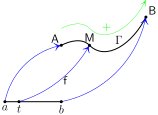
\includegraphics{./asy/fig20230207150452.pdf}

}

\caption{\label{fig-20230207150452}La courbe \(\Gamma\) est paramétrée
par \(\point{f}\).}

\end{figure}

On supposera dans ce qui suit l'application \(\point{f}\) suffisamment
régulière (en général, au moins une fois continûment dérivable par
morceaux) pour que toutes les relations faisant intervenir \(\point{f}\)
et ses dérivées aient un sens. En particulier, l'application
\(\point{f}\) est \emph{continue}: la courbe décrite par \(\point{f}\)
dans \(\reals^d\) est donc elle-même continue au sens usuel du terme :
on trace cette courbe sans lever le crayon.

Le choix du paramétrage \(t \mapsto \point{f}(t)\) définit naturellement
une \emph{orientation} de la courbe \(\Gamma\), de son \emph{origine}
\(\point{A} = \point{f}(a)\) vers son extrémité
\(\point{B} = \point{f}(b)\). Toute application
\(\Phi\colon [a', b'] \longleftrightarrow [a, b]\) strictement
croissante et régulière permet de définir le nouveau paramétrage
\(\point{f} \circ \Phi\) de la courbe \(\Gamma\). Dans ce changement de
paramètre, l'orientation de la courbe est préservée.

\begin{tcolorbox}[enhanced jigsaw, toptitle=1mm, title=\textcolor{quarto-callout-note-color}{\faInfo}\hspace{0.5em}{Note}, colbacktitle=quarto-callout-note-color!10!white, toprule=.15mm, left=2mm, bottomrule=.15mm, arc=.35mm, breakable, opacityback=0, colframe=quarto-callout-note-color-frame, bottomtitle=1mm, titlerule=0mm, leftrule=.75mm, opacitybacktitle=0.6, coltitle=black, rightrule=.15mm, colback=white]

Dans le plan (\(d = 2\)) et dans l'espace (\(d = 3\)), respectivement,
l'application \(\point{f}\) est définie par les \emph{équations
paramétriques} \((x(t), y(t))\) et \(x(t), y(t), z(t)\), respectivement,
de la courbe \(\Gamma\) \[
\point{f}(t) = \begin{bmatrix} x(t) \\ y(t) \end{bmatrix}
\quad \text{et} \quad
\point{f}(t) = \begin{bmatrix} x(t) \\ y(t) \\ z(t) \end{bmatrix}.
\]

\end{tcolorbox}

\hypertarget{tangente}{%
\subsection{Tangente}\label{tangente}}

Notion intuitive : soit \(\point{M} = \point{f}(t) \in \Gamma\) fixé. On
considère le point \(\point{M'} = \point{f}(t')\), voisin de
\(\point{M}\). La droite \((\point{MM}')\) définit une \emph{sécante} à
la courbe \(\Gamma\). Lorsque \(\point{M}'\) «~se rapproche de
\(\point{M}\)~» (voir Figure~\ref{fig-20230207155607} ), cette sécante
se rapproche de la \emph{tangente} à \(\Gamma\) en \(\point{M}\) qui est
donc définie comme la droite passant par \(\point{M}\) et de vecteur
directeur \[
\lim_{t' \to t} \frac{\altvec{\point{MM}'}}{t' - t} = \lim_{t' \to t} \frac{\point{M'} - \point{M}}{t' - t} = \dot{\point{f}}(t),
\] où le point désigne la dérivée par rapport au paramètre \(t\). Le
vecteur \(\dot{\point{f}}(t)\) est donc un vecteur tangent au point
\(\point{f}(t)\) de la courbe \(\Gamma\).

\begin{figure}

{\centering 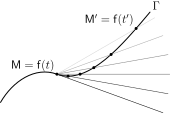
\includegraphics{./asy/fig20230207155607.pdf}

}

\caption{\label{fig-20230207155607}Construction de la tangente à la
courbe \(\Gamma\) au point \(\point{M}\).}

\end{figure}

\begin{tcolorbox}[enhanced jigsaw, toptitle=1mm, title=\textcolor{quarto-callout-note-color}{\faInfo}\hspace{0.5em}{Note}, colbacktitle=quarto-callout-note-color!10!white, toprule=.15mm, left=2mm, bottomrule=.15mm, arc=.35mm, breakable, opacityback=0, colframe=quarto-callout-note-color-frame, bottomtitle=1mm, titlerule=0mm, leftrule=.75mm, opacitybacktitle=0.6, coltitle=black, rightrule=.15mm, colback=white]

On vérifie aisément que la droite tangente ainsi définie est invariante
par changement de paramètre.

\end{tcolorbox}

\begin{tcolorbox}[enhanced jigsaw, toptitle=1mm, title=\textcolor{quarto-callout-note-color}{\faInfo}\hspace{0.5em}{Note}, colbacktitle=quarto-callout-note-color!10!white, toprule=.15mm, left=2mm, bottomrule=.15mm, arc=.35mm, breakable, opacityback=0, colframe=quarto-callout-note-color-frame, bottomtitle=1mm, titlerule=0mm, leftrule=.75mm, opacitybacktitle=0.6, coltitle=black, rightrule=.15mm, colback=white]

Les coordonnées du vecteur tangent, sont en dimensions 2 et 3,
respectivement \[
\dot{\point{f}}(t) = \begin{bmatrix} \dot{x}(t) \\ \dot{y}(t) \end{bmatrix}
\quad \text{et} \quad
\dot{\point{f}}(t) = \begin{bmatrix} \dot{x}(t) \\ \dot{y}(t) \\ \dot{z}(t) \end{bmatrix}.
\]

\end{tcolorbox}

\hypertarget{rectification-dune-courbe}{%
\subsection{Rectification d'une
courbe}\label{rectification-dune-courbe}}

On cherche à calculer la longueur de l'arc \(\point{AB}\). À cet effet,
on approxime l'arc par une ligne polygonale
\(\point{M}_0 = \point{A}, \point{M_1}, \ldots, \point{M_n} = \point{B}\),
où \(\point{M}_k\) est le point de \(\Gamma\) d'antécédent \(t_k\) par
\(\point{f}\) (\(t_0 < t_1 < \cdots < t_n\)). La longueur de cette ligne
polygonale est (voir Figure~\ref{fig-20230207181908})

\[
\sum _ {k = 0} ^ {n - 1} \bigl \lVert \point{M} _ {k+1} - \point{M} _ k \bigr \rVert
= \sum _ {k = 0} ^ {n - 1} \bigl \lVert  \point{f}(t _ {k+1}) - \point{M}(t _ k) \bigr \rVert
\]

\begin{figure}

{\centering 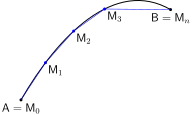
\includegraphics{./asy/fig20230207181908.pdf}

}

\caption{\label{fig-20230207181908}Approximation de l'arc \(\point{AB}\)
construit sur \(\Gamma\) par une ligne brisée.}

\end{figure}

Si les points \(\point{M}_k\) sont suffisamment rapprochés, on peut
remplacer la sécante par la tangente \[
\sum _ {k = 0} ^ {n - 1} \bigl \lVert \point{M} _ {k+1} - \point{M} _ k \bigr \rVert
\simeq \sum _ {k = 0} ^ {n - 1} \bigl \lVert \dot{\point{f}}(t _ k) \bigr \rVert \, \bigl ( t _ {k+1} - t _ k \bigr)
\] et la somme discrète par une intégrale \[
\sum _ {k = 0} ^ {n - 1} \bigl \lVert \point{M} _ {k+1} - \point{M} _ k \bigr \rVert
\simeq \int _ {a} ^ {b} \bigl \lVert  \dot{\point{f}}(t) \bigr \rVert \, \D t.
\]

L'intégrale ci-dessus est la longueur de l'arc \(\point{AB}\) tracé sur
la courbe \(\Gamma\)
\begin{equation}\protect\hypertarget{eq-20230207112239}{}{
\mathcal{L} _ \Gamma(\point{A}, \point{B}) = \int _ {a} ^ {b} \bigl \lVert  \dot{\point{f}}(t) \bigr \rVert \, \D t.
}\label{eq-20230207112239}\end{equation}

\begin{tcolorbox}[enhanced jigsaw, toptitle=1mm, title=\textcolor{quarto-callout-note-color}{\faInfo}\hspace{0.5em}{Note}, colbacktitle=quarto-callout-note-color!10!white, toprule=.15mm, left=2mm, bottomrule=.15mm, arc=.35mm, breakable, opacityback=0, colframe=quarto-callout-note-color-frame, bottomtitle=1mm, titlerule=0mm, leftrule=.75mm, opacitybacktitle=0.6, coltitle=black, rightrule=.15mm, colback=white]

On vérifie aisément que cette expression est invariante par changement
de paramètre.

\end{tcolorbox}

On peut de même mesurer pour tout point \(\point{M}\) situé entre
\(\point{A}\) et \(\point{B}\), la longueur de l'arc \(\point{AB}\) :
c'est \emph{l'abscisse curviligne} \(s\) du point \(\point{M}\),
l'origine étant fixée en \(\point{A}\) :
\(s = \mathcal{L}_\Gamma(\point{A}, \point{M})\). On définit ainsi une
application \(\Psi \colon [a, b] \longrightarrow [0, L]\) \[
 s = \Psi(t) = \int_a^t \bigl \lVert  \dot{\point{f}}(u) \bigr \rVert \, \D u.
\]

La fonction ainsi définie étant croissante et suffisamment régulière,
elle est inversible : \(t = \Phi(s)\). L'application
\(\point{f} \circ \Phi\) définit un paramétrage particulier de la courbe
par l'abscisse curviligne \(s\). On dit qu'on a \emph{rectifié} la
courbe \(\Gamma\).

\begin{tcolorbox}[enhanced jigsaw, toptitle=1mm, title=\textcolor{quarto-callout-note-color}{\faInfo}\hspace{0.5em}{Note}, colbacktitle=quarto-callout-note-color!10!white, toprule=.15mm, left=2mm, bottomrule=.15mm, arc=.35mm, breakable, opacityback=0, colframe=quarto-callout-note-color-frame, bottomtitle=1mm, titlerule=0mm, leftrule=.75mm, opacitybacktitle=0.6, coltitle=black, rightrule=.15mm, colback=white]

La définition (\ref{eq-20230207112239}) est \emph{algébrique}. Plus
précisément, si on choisit pour origine des abscisses curvilignes le
point \(\point{C}\) de paramètre \(c\) (\(a < c < b\)), alors l'abscisse
curviligne \(\int_c^t \lVert \dot{\point{f}}(t) \rVert \, \D t\) du
point \(\point{M} = \point{f}(t)\) est \emph{négative} si \(\point{M}\)
est entre \(\point{A}\) et \(\point{C}\) (\(a \leq t \leq c\)), et
\emph{positive} si \(\point{M}\) est entre \(\point{C}\) et
\(\point{B}\) (\(c \leq t \leq b\)).

\end{tcolorbox}

\hypertarget{sec-20230207114551}{%
\subsection{Vecteur tangent unitaire}\label{sec-20230207114551}}

On suppose la courbe \(\Gamma\) rectifiée, et on note
\(s \mapsto \point{f}(s)\) le paramétrage associé. Le vecteur
\(\vec{t} = \point{f}'(s)\) est \emph{tangent} à \(\Gamma\) au point
\(\point{M} = \point{f}(s)\) (voir @).

\begin{figure}

{\centering 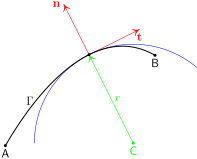
\includegraphics{./asy/fig20230207190019.pdf}

}

\caption{\label{fig-20230207190019}Les vecteurs unitaires \(\vec t\) et
\(\vec n\) forment la base de Frénet. Le point \(C\) est le centre de
courbure, et le cercle bleu est le cercle osculateur en \(\point{M}\).}

\end{figure}

On vérifie aisément que ce vecteur est unitaire. En effet, la longueur
de l'arc \(\point{AM}\) tracé sur \(\Gamma\) s'écrit \[
\mathcal{L}_\Gamma(\point{A}, \point{M}) = \int_a^s \bigl \lVert  \dot{\point{f}}(u) \bigr \rVert \, \D u.
\] où le paramètre est l'abscisse curviligne \(s\), qui est par
définition égale ) \(\mathcal{L}_\Gamma(\point{A}, \point{M})\). On a
donc, pour tout \(s\) \[
s = \int_a^s \bigl \lVert  \dot{\point{f}}(u) \bigr \rVert \, \D u,
\] d'où il résulte que \(\lVert \vec t \rVert = 1\). Le vecteur
\(\vec t\) est le \emph{vecteur tangent unitaire} à la courbe \(\Gamma\)
au point \(\point{M}\). Il sera parfois commode de repérer ce vecteur
par l'angle \(\theta\) qu'il fait par rapport à une direction fixe
arbitraire (typiquement, \(\vec e_x\))
\begin{equation}\protect\hypertarget{eq-20230207121436}{}{
\vec t(s) = \cos \theta(s) \, \vec e_x + \sin \theta(s) \, \vec e_y.
}\label{eq-20230207121436}\end{equation}

\hypertarget{sec-20230214055209}{%
\section{Courbure des courbes planes}\label{sec-20230214055209}}

Dans ce paragraphe, on considère le cas d'une courbe plane (\(d = 2\)),
dont on définit la \emph{courbure}. Les résultats présentés peuvent être
étendus aux courbes \emph{gauches} (\(d = 3\)) en introduisant également
la notion de \emph{torsion}, dont nous n'aurons pas besoin dans ce
cours.

Le vecteur tangent \(\vec t\) unitaire étant défini en tout point de la
courbe, on peut également définir le \emph{vecteur normal unitaire}
\(\vec n\), qui lui est perpendiculaire.

\begin{tcolorbox}[enhanced jigsaw, toptitle=1mm, title=\textcolor{quarto-callout-note-color}{\faInfo}\hspace{0.5em}{Note}, colbacktitle=quarto-callout-note-color!10!white, toprule=.15mm, left=2mm, bottomrule=.15mm, arc=.35mm, breakable, opacityback=0, colframe=quarto-callout-note-color-frame, bottomtitle=1mm, titlerule=0mm, leftrule=.75mm, opacitybacktitle=0.6, coltitle=black, rightrule=.15mm, colback=white]

Deux orientations sont possibles pour le vecteur \(\vec n\). Il est
important de remarquer qu'il n'y a pas de choix \emph{canonique} : il
sera donc toujours nécessaire de \textbf{préciser l'orientation de la
normale}.

\end{tcolorbox}

\hypertarget{premiuxe8re-formule-de-fruxe9net}{%
\subsection{Première formule de
Frénet}\label{premiuxe8re-formule-de-fruxe9net}}

Au point \(\point{M}\) de la courbe \(\Gamma\), le vecteur \(\vec{t}\)
défini au §§~\ref{sec-20230207114551} est unitaire. Sa dérivée
\(\vec{t}'\) lui est perpendiculaire. En effet \[
\vec t \cdot \vec t = 1 \quad \text{donc} \quad 0 = \frac{\D}{\D s} \bigl( \vec t \cdot \vec t \bigr) = 2 \vec t \cdot \vec t'.
\]

En d'autres termes, \(\vec t'\) est porté par \(\vec n\). On introduit
le scalaire \(\kappa\) tel que \[
\vec t' = \frac{\D \vec{t}}{\D s} = \kappa \, \vec n
\] (première formule de Frénet). \(\kappa\) est homogène à l'inverse
d'une longueur. C'est la \emph{courbure de \(\Gamma\) en \(\point{M}\)}.
Son inverse, \(r = \kappa^{-1}\) est le \emph{rayon de courbure}. On
montre en effet que le cercle de centre \(\point{M} + r \, \vec{n}\) et
de rayon \(\lvert r \rvert\) est celui qui approche le mieux la courbe
\(\Gamma\) au voisinage de \(\point{M}\) (cercle osculateur).

\begin{tcolorbox}[enhanced jigsaw, toptitle=1mm, title=\textcolor{quarto-callout-note-color}{\faInfo}\hspace{0.5em}{Note}, colbacktitle=quarto-callout-note-color!10!white, toprule=.15mm, left=2mm, bottomrule=.15mm, arc=.35mm, breakable, opacityback=0, colframe=quarto-callout-note-color-frame, bottomtitle=1mm, titlerule=0mm, leftrule=.75mm, opacitybacktitle=0.6, coltitle=black, rightrule=.15mm, colback=white]

La courbure est une grandeur \emph{algébrique}, dont \textbf{le signe
n'est pas intrinsèque} : il dépend de l'orientation de la normale
\(\vec n\), qui est arbitraire. En effet, changer \(\vec n\) en
\(-\vec n\) conduit à remplacer la courbure \(\kappa\) par son opposé
\(-\kappa\).

Les vecteurs \(\kappa \, \vec n\) et \(r \, \vec n\) sont quant à eux
bien intrinsèques. Ils pointent vers le centre de courbure.

\textbf{Traiter l'exemple du cercle en cours}

\end{tcolorbox}

\hypertarget{deuxiuxe8me-formule-de-fruxe9net}{%
\subsection{Deuxième formule de
Frénet}\label{deuxiuxe8me-formule-de-fruxe9net}}

Par construction, le vecteur normal unitaire \(\vec n\) est de norme
constante : sa dérivée lui est donc perpendiculaire, et \(\vec n'\) est
parallèle à \(\vec t\). On introduit le scalaire \(\alpha\) tel que
\(\vec n' = \alpha \, \vec t\). Comme \(\vec t\) et \(\vec n\) sont
perpendiculaires, on a \(\vec t \cdot \vec n = 0\), soit, en dérivant \[
0 = \vec t' \cdot \vec n + \vec t \cdot \vec n' = \kappa \, \vec n \cdot \vec n + \alpha \, \vec t \cdot \vec t = \kappa + \alpha
\] et \(\alpha = -\kappa\). On a ainsi obtenu la deuxième formule de
Frénet \[
\vec n' = \frac{\D \vec{n}}{\D s} = -\kappa \, \vec t.
\]

\hypertarget{lien-avec-la-direction-de-la-tangente}{%
\subsection{Lien avec la direction de la
tangente}\label{lien-avec-la-direction-de-la-tangente}}

L'angle \(\theta(s)\) a été défini plus haut par la relation
(\ref{eq-20230207121436}). En dérivant cette relation, on obtient \[
\kappa \, \vec n = \vec t' = \theta'(s) \, \bigl[ -\sin \theta(s) \, \vec e_x + \cos \theta(s) \, \vec e_y \bigr]
\]

Le vecteur entre crochets est un vecteur unitaire, \emph{directement
perpendiculaire} à \(\vec t\). Donc

\begin{itemize}
\tightlist
\item
  \(\kappa = \theta'\) si \((\vec t, \vec n)\) est une base directe,
\item
  \(\kappa = -\theta'\) si \((\vec n, \vec t)\) est une base directe.
\end{itemize}

\hypertarget{compluxe9ments-dalguxe8bre-linuxe9aire}{%
\chapter{Compléments d'algèbre
linéaire}\label{compluxe9ments-dalguxe8bre-linuxe9aire}}

\hypertarget{sec-20230213110532}{%
\section{Application linéaire entre deux plans de
l'espace}\label{sec-20230213110532}}

Dans ce paragraphe, on considère \emph{deux} plans de l'espace, \(\Pi\)
et \(\pi\), leurs normales unitaires \(\vec N\) et \(\vec n\) et les
opérateurs de projection associés \(\tens A\) et \(\tens a\). Soit
\(\vec{f}\) une application linéaire de \(\Pi\) sur \(\pi\). Pour tout
\(\vec V \in \Pi\), on a \(\vec n \cdot \vec{f}(\vec V) = 0\), puisque
\(\vec{f}(\vec V) \in \pi\) par construction. L'application linéaire
\(\vec{f}\), définie seulement sur \(\Pi\), peut être prolongée sur
l'espace \(\reals^3\) tout entier en convenant que
\(\vec{f}(\vec N) = \vec{0}\). En d'autres termes, on pose \[
\vec{f}(\vec{V}) = \vec{f}(\tens A \cdot \vec{V}) \quad (\vec V \in \reals^3).
\]

On a ainsi défini un \emph{endomorphisme} de l'espace \(\reals^3\),
auquel on peut associer le tenseur \(\tens F\). Par construction,
\(\vec{f}(\vec{N}) = \vec{0}\); par ailleurs, l'image par \(\vec{f}\) de
tout vecteur de l'espace est contenue dans le plan \(\pi\). En d'autres
termes, pour tout \(\vec{V} \in \reals^3\),
\(\vec{n} \cdot \vec{f}(\vec V) = \vec{0}\). On en déduit donc les
relations importantes
\begin{equation}\protect\hypertarget{eq-20230210152426}{}{
\tens F \cdot \vec N = \vec n \cdot \tens F = \vec 0.
}\label{eq-20230210152426}\end{equation}

Inversement, un tenseur \(\tens F\) d'ordre deux de l'espace
satisfaisant les relations précédentes peut être vu comme une
application linéaire de \(\Pi\) sur \(\pi\).

Compte-tenu de la première des relations (\ref{eq-20230210152426}), le
tenseur \(\tens F\) n'est bien sûr pas inversible dans l'espace. Son
déterminant n'apporte donc aucune information, puisqu'il est nul. On
montrera en revanche que le déterminant du tenseur
\(\tens F + \vec n \otimes \vec N\) permet de mesurer des variations
d'aire au cours de la transformation d'une coque. On a en effet la
relation suivante, valable pour tous vecteurs
\(\vec{V}, \vec{W} \in \reals^3\) de l'espace \[
\vec n \cdot \bigl[ \bigl( \tens F \cdot \vec V \bigr) \times \bigl( \tens F \cdot \vec W \bigr) \bigr]
= \vec N \cdot \bigl( \vec V \times \vec W \bigr) \, \det\bigl( \tens F + \vec n \otimes \vec N \bigr).
\]

\begin{tcolorbox}[enhanced jigsaw, opacityback=0, colframe=quarto-callout-tip-color-frame, colback=white, toprule=.15mm, rightrule=.15mm, left=2mm, leftrule=.75mm, bottomrule=.15mm, arc=.35mm, breakable]

Soient \(\tens{F}^\sharp = \tens{F} + \vec{n} \otimes \vec{N}\) et
\(\vec{V}\) et \(\vec{W}\) deux vecteurs quelconques de l'espace. Par
construction de \(\tens{F}\), on a
\(\tens{F} \cdot \vec{V} = \tens{F} \cdot \bigl( \tens A \cdot \vec{V} \bigr)\).
Puisque \(\tens{A} \cdot \vec{V} \in \Pi\), on a
\(\tens{F}^\sharp \cdot \bigl( \tens{A} \cdot \vec{V} \bigr) = \tens{F} \cdot \bigl( \tens{A} \cdot \vec{V} \bigr) = \tens{F} \cdot \vec{V}\)
(relations similaires pour \(\vec{W}\)). En observant par ailleurs que
\(\tens{F}^\sharp \cdot \vec{N} = \vec{n}\) et en reconnaissant un
produit mixte, on obtient \[
\begin{aligned}
\vec{n} \cdot \bigl[ \bigl( \tens{F} \cdot \vec{V} \bigr) \times \bigl( \tens{F} \cdot \vec{W} \bigr) \bigr]
&= \bigl[\tens{F}^\sharp \cdot \vec{N}, \tens{F}^\sharp \cdot \bigl( \tens{A} \cdot \vec{V} \bigr), \tens{F}^\sharp \cdot \bigl( \tens{A} \cdot \vec{W} \bigr) \bigr]\\
&= \bigl[ \vec{N}, \tens{A} \cdot \vec{V}, \tens{A} \cdot \vec{W} \bigr] \, \det \tens F^\sharp.
\end{aligned}
\]

Enfin, en remarquant que
\(\tens{A} \cdot \vec{V} = \vec{V} - \bigl( \vec{V} \cdot \vec N \bigr) \, \vec{N}\)
\[
\begin{aligned}
\bigl[ \vec{N}, \tens{A} \cdot \vec{V}, \tens{A} \cdot \vec{W} \bigr]
= {} &
\bigl[ \vec{N}, \vec{V} - \bigl( \vec{V} \cdot \vec N \bigr) \, \vec{N}, \vec{W} - \bigl( \vec{W} \cdot \vec N \bigr) \, \vec{N} \bigr]\\
= {} & \bigl[ \vec{N}, \vec{V}, \vec{W} \bigr] - \bigl( \vec{V} \cdot \vec N \bigr) \, \bigl[ \vec{N}, \vec{N}, \vec{W} \bigr] - \bigl( \vec{W} \cdot \vec N \bigr) \, \bigl[ \vec{N}, \vec{V}, \vec{N} \bigr]\\
    & + \bigl( \vec{V} \cdot \vec N \bigr) \, \bigl( \vec{W} \cdot \vec N \bigr) \, \bigl[ \vec{N}, \vec{N}, \vec{N} \bigr] =  \bigl[ \vec{N}, \vec{V}, \vec{W} \bigr],
\end{aligned}
\] puisque
\(\bigl[ \vec{N}, \vec{N}, \vec{W} \bigr] = \bigl[ \vec{N}, \vec{V}, \vec{N} \bigr] = \bigl[ \vec{N}, \vec{N}, \vec{N} \bigr] = 0\).

\end{tcolorbox}

Vu comme un endomorphisme de l'espace, \(\tens{F}\) n'est \emph{jamais
inversible}. En revanche, il peut être le représentant d'une application
linéaire inversible entre les plans \(\Pi\) et \(\pi\). On notera
\(\tens F^\dagger\) son inverse. En d'autres termes, pour tous
\(\vec{V} \in \Pi\) et \(\vec{v} \in \pi\), on a \[
\vec{v} = \tens{F} \cdot \vec{V} \quad \text{ssi} \quad \vec{V} = \tens{F}^\dagger \cdot \vec{v},
\] que l'on peut également résumer par les relations suivantes \[
\tens{F}^\dagger \cdot \tens{F} = \tens{A} \quad \text{et} \quad \tens{F} \cdot \tens{F}^\dagger = \tens{a}.
\]

\begin{tcolorbox}[enhanced jigsaw, toptitle=1mm, title=\textcolor{quarto-callout-note-color}{\faInfo}\hspace{0.5em}{Note}, colbacktitle=quarto-callout-note-color!10!white, toprule=.15mm, left=2mm, bottomrule=.15mm, arc=.35mm, breakable, opacityback=0, colframe=quarto-callout-note-color-frame, bottomtitle=1mm, titlerule=0mm, leftrule=.75mm, opacitybacktitle=0.6, coltitle=black, rightrule=.15mm, colback=white]

Le tenseur \(\tens{F}^\dagger\) n'est pas l'inverse du tenseur (de
l'espace) \(\tens{F}\). C'est l'extension à tout l'espace de l'inverse
de la restriction de \(\tens{F}\) aux plans \(\Pi\) (espace de départ)
et \(\pi\) (espace d'arrivée). On parle alors de
\textbf{pseudo-inverse}\footnote{\url{https://fr.wikipedia.org/wiki/Pseudo-inverse},
  visité le 10/02/2023.} de \(\tens{F}\).

On peut facilement montrer que \(\tens{F}\) admet une pseudo-inverse si,
et seulement si, \(\tens{F} + \vec{n} \otimes \vec{N}\) est inversible,
c'est-à-dire
\(\det\bigl( \tens F + \vec n \otimes \vec N \bigr) \neq 0\). Dans ce
cas, on a \[
\bigl( \tens{F} + \vec{n} \otimes \vec{N} \bigr)^{-1} = \tens{F}^\dagger + \vec{N} \otimes \vec{n}.
\]

\end{tcolorbox}

\begin{tcolorbox}[enhanced jigsaw, opacityback=0, colframe=quarto-callout-tip-color-frame, colback=white, toprule=.15mm, rightrule=.15mm, left=2mm, leftrule=.75mm, bottomrule=.15mm, arc=.35mm, breakable]

Il suffit de former les produits suivants \[
\begin{aligned}
\bigl( \tens{F} + \vec{n} \otimes \vec{N} \bigr) \cdot \bigl( \tens{F}^\dagger + \vec{N} \otimes \vec{n} \bigr)
&= \tens{F} \cdot \tens{F}^\dagger + \bigl( \tens{F} \cdot \vec{N} \bigr) \otimes \vec{n} + \vec{n} \otimes \bigl( \vec{N} \cdot \tens{F}^\dagger \bigr) + \vec{n} \otimes \vec{n}\\
&= \tens{a} + \vec{n} \otimes \vec{n} = \tens{I},
\end{aligned}
\] et \[
\begin{aligned}
\bigl( \tens{F}^\dagger + \vec{N} \otimes \vec{n} \bigr) \cdot \bigl( \tens{F} + \vec{n} \otimes \vec{N} \bigr)
&= \tens{F}^\dagger \cdot \tens{F} +\bigl( \tens{F}^\dagger \cdot \vec{n} \bigr) \otimes \vec{N} + \vec{N} \otimes \bigl( \vec{n} \cdot \tens{F} \bigr) + \vec{N} \otimes \vec{N}\\
&= \tens{A} + \vec{N} \otimes \vec{N} = \tens{I}.
\end{aligned}
\]

\end{tcolorbox}

\begin{tcolorbox}[enhanced jigsaw, toptitle=1mm, title=\textcolor{quarto-callout-note-color}{\faInfo}\hspace{0.5em}{Note}, colbacktitle=quarto-callout-note-color!10!white, toprule=.15mm, left=2mm, bottomrule=.15mm, arc=.35mm, breakable, opacityback=0, colframe=quarto-callout-note-color-frame, bottomtitle=1mm, titlerule=0mm, leftrule=.75mm, opacitybacktitle=0.6, coltitle=black, rightrule=.15mm, colback=white]

Lorsque les plans \(\Pi\) et \(\pi\) sont confondus, le tenseur
\(\tens{F}\) peut être vu comme un \emph{endomorphisme} du plan, pour
lequel la notion de déterminant (\(2 \times 2\)) a un sens. Dans ce cas
\[
\det_{2 \times 2} \tens F = \det_{3 \times 3} \bigl( \tens F + \vec N \otimes \vec N \bigr).
\]

\end{tcolorbox}



\end{document}
